% !TeX spellcheck = hu_HU
% !TeX encoding = UTF-8
% !TeX program = xelatex

\PassOptionsToPackage{hyphens}{url}
\documentclass[11pt,a4paper,oneside]{report}             % Single-side
%\documentclass[11pt,a4paper,twoside,openright]{report}  % Duplex

% thanks to http://tex.stackexchange.com/a/47579/71109
\usepackage{ifxetex}
\usepackage{ifluatex}

\newif\ifxetexorluatex % a new conditional starts as false
\ifnum 0\ifxetex 1\fi\ifluatex 1\fi>0
   \xetexorluatextrue
\fi

\ifxetexorluatex
  \usepackage{fontspec}
  % xelatex-nél elég a fontspec include-olása
  % lásd: https://tex.stackexchange.com/questions/462664/warnings-when-using-babel-with-lualatex
  \def\magyarOptions{suggestions=no}
\else
  \usepackage[T1]{fontenc}
  \usepackage[utf8]{inputenc}
  \usepackage[lighttt]{lmodern}
\fi

\usepackage[magyar]{babel} % Alapértelmezés szerint utoljára definiált nyelv lesz aktív, de később külön beállítjuk az aktív nyelvet.

%\usepackage{cmap}
\usepackage{amsfonts,amsmath,amssymb} % Mathematical symbols.
%\usepackage[ruled,boxed,resetcount,linesnumbered]{algorithm2e} % For pseudocodes. % beware: this is not compatible with LuaLaTeX, see http://tex.stackexchange.com/questions/34814/lualatex-and-algorithm2e
\usepackage{booktabs} % For publication quality tables for LaTeX
\usepackage{graphicx}
\usepackage{subcaption}

%\usepackage{fancyhdr}
%\usepackage{lastpage}

\usepackage{anysize}
%\usepackage{sectsty}
\usepackage{setspace} % For setting line spacing

\usepackage[unicode]{hyperref} % For hyperlinks in the generated document.
\usepackage{xcolor}
\usepackage{listings} % For source code snippets.

% https://tex.stackexchange.com/a/224743
\lstset{
	basicstyle=\ttfamily,
	keepspaces=true,
	escapeinside={(*@}{@*)}, % only required for XeLaTeX
	columns=flexible, % only use with keepspaces=true       
	literate=*
	{á}{{\'a}}1
	{é}{{\'e}}1
	{í}{{\'i}}1
	{ó}{{\'o}}1
	{ö}{{\"o}}1
	{ő}{{\H{o}}}1
	{ú}{{\'u}}1
	{ü}{{\"u}}1
	{ű}{{\H{u}}}1
	{Á}{{\'A}}1
	{É}{{\'E}}1
	{Í}{{\'I}}1
	{Ó}{{\'O}}1
	{Ö}{{\"O}}1
	{Ő}{{\H{O}}}1
	{Ú}{{\'U}}1
	{Ü}{{\"U}}1
	{Ű}{{\H{U}}}1
}


\usepackage[amsmath,thmmarks]{ntheorem} % Theorem-like environments.

%\usepackage[hang]{caption}

\usepackage{array}
\usepackage{extdash}

\usepackage{tikz}
\usetikzlibrary{shadows}

% roviditesjegyzek
\usepackage[toc, acronyms]{glossaries}
\usepackage{makeidx}
\usepackage{tocbibind}

\makeglossaries
\makeindex


\singlespacing

\newcommand{\selecthungarian}{
	\selectlanguage{magyar}
	\setlength{\parindent}{2em}
	\setlength{\parskip}{0em}
	\frenchspacing
}

\newcommand{\selectenglish}{
	\selectlanguage{english}
	\setlength{\parindent}{0em}
	\setlength{\parskip}{0.5em}
	\nonfrenchspacing
	\renewcommand{\figureautorefname}{Figure}
	\renewcommand{\tableautorefname}{Table}
	\renewcommand{\partautorefname}{Part}
	\renewcommand{\chapterautorefname}{Chapter}
	\renewcommand{\sectionautorefname}{Section}
	\renewcommand{\subsectionautorefname}{Section}
	\renewcommand{\subsubsectionautorefname}{Section}
}

\usepackage[numbers]{natbib}
\usepackage{xspace}

\newcommand{\vikszerzoVezeteknev}{Főglein}
\newcommand{\vikszerzoKeresztnev}{Simon István}

\newcommand{\vikkonzulensAMegszolitas}{dr.~}
\newcommand{\vikkonzulensAVezeteknev}{Somogyi}
\newcommand{\vikkonzulensAKeresztnev}{Péter}

\newcommand{\vikkonzulensBMegszolitas}{}
\newcommand{\vikkonzulensBVezeteknev}{}
\newcommand{\vikkonzulensBKeresztnev}{}

\newcommand{\vikkonzulensCMegszolitas}{}
\newcommand{\vikkonzulensCVezeteknev}{}
\newcommand{\vikkonzulensCKeresztnev}{}

\newcommand{\vikcim}{Kiszolgálók üzemeltetése nagyvállalati környezetben és kapcsolódó szoftverek fejlesztése} % Cím
\newcommand{\viktanszek}{\bmeiit} % Tanszék
\newcommand{\vikdoktipus}{\bsc} % Dokumentum típusa (\bsc vagy \msc)
\newcommand{\vikmunkatipusat}{szakdolgozatot} % a "hallgató nyilatkozat" részhez: szakdolgozatot vagy diplomatervet

%--------------------------------------------------------------------------------------
% TDK-specifikus változók
%--------------------------------------------------------------------------------------
\newcommand{\tdkszerzoB}{Második Szerző} % Második szerző neve; hagyd üresen, ha egyedül írtad a TDK-t.
\newcommand{\tdkev}{2014} % A dolgozat írásának éve (pl. "2014") (Ez OTDK-nál eltérhet az aktuális évtől.)

% További adatok az OTDK címlaphoz (BME-s TDK-hoz nem kell kitölteni)
\newcommand{\tdkevfolyamA}{IV} % Első szerző évfolyama, római számmal (pl. IV).
\newcommand{\tdkevfolyamB}{III} % Második szerző évfolyama, római számmal (pl. III).
\newcommand{\tdkkonzulensbeosztasA}{egyetemi tanár} % Első konzulens beosztása (pl. egyetemi docens)
\newcommand{\tdkkonzulensbeosztasB}{doktorandusz} % Második konzulens beosztása (pl. egyetemi docens)

\newcommand{\szerzoMeta}{\vikszerzoVezeteknev{} \vikszerzoKeresztnev} % egy szerző esetén
%\newcommand{\szerzoMeta}{\vikszerzoVezeteknev{} \vikszerzoKeresztnev, \tdkszerzoB} % két szerző esetén

% Beállítások magyar nyelvű dolgozathoz
%--------------------------------------------------------------------------------------
% Elnevezések
%--------------------------------------------------------------------------------------
\newcommand{\bme}{Budapesti Műszaki és Gazdaságtudományi Egyetem}
\newcommand{\vik}{Villamosmérnöki és Informatikai Kar}

\newcommand{\bmemit}{Méréstechnika és Információs Rendszerek Tanszék}
\newcommand{\bmeiit}{Irányítástechnika és Informatika Tanszék}

\newcommand{\keszitette}{Készítette}
\newcommand{\konzulens}{Konzulens}

\newcommand{\bsc}{Szakdolgozat}
\newcommand{\msc}{Diplomaterv}
\newcommand{\tdk}{TDK dolgozat}
\newcommand{\bsconlab}{BSc Önálló laboratórium}
\newcommand{\msconlabi}{MSc Önálló laboratórium 1.}
\newcommand{\msconlabii}{MSc Önálló laboratórium 2.}

\newcommand{\pelda}{Példa}
\newcommand{\definicio}{Definíció}
\newcommand{\tetel}{Tétel}

\newcommand{\bevezetes}{Bevezetés}
\newcommand{\koszonetnyilvanitas}{Köszönetnyilvánítás}
\newcommand{\fuggelek}{Függelék}

% Opcionálisan átnevezhető címek
%\addto\captionsmagyar{%
%\renewcommand{\listfigurename}{Saját ábrajegyzék cím}
%\renewcommand{\listtablename}{Saját táblázatjegyzék cím}
%\renewcommand{\bibname}{Saját irodalomjegyzék név}
%}

\newcommand{\szerzo}{\vikszerzoVezeteknev{} \vikszerzoKeresztnev}
\newcommand{\vikkonzulensA}{\vikkonzulensAMegszolitas\vikkonzulensAVezeteknev{} \vikkonzulensAKeresztnev}
\newcommand{\vikkonzulensB}{\vikkonzulensBMegszolitas\vikkonzulensBVezeteknev{} \vikkonzulensBKeresztnev}
\newcommand{\vikkonzulensC}{\vikkonzulensCMegszolitas\vikkonzulensCVezeteknev{} \vikkonzulensCKeresztnev}

\newcommand{\selectthesislanguage}{\selecthungarian}

\bibliographystyle{huplain}

\def\lstlistingname{lista}

\newcommand{\appendixnumber}{6}  % a fofejezet-szamlalo az angol ABC 6. betuje (F) lesz

% Settings for English documents
%%--------------------------------------------------------------------------------------
% Elnevezések
%--------------------------------------------------------------------------------------
\newcommand{\bme}{Budapest University of Technology and Economics}
\newcommand{\vik}{Faculty of Electrical Engineering and Informatics}

\newcommand{\bmemit}{Department of Measurement and Information Systems}

\newcommand{\keszitette}{Author}
\newcommand{\konzulens}{Advisor}

\newcommand{\bsc}{Bachelor's Thesis}
\newcommand{\msc}{Master's Thesis}
\newcommand{\tdk}{Scientific Students' Association Report}
\newcommand{\bsconlab}{BSc Project Laboratory}
\newcommand{\msconlabi}{MSc Project Laboratory 1}
\newcommand{\msconlabii}{MSc Project Laboratory 2}

\newcommand{\pelda}{Example}
\newcommand{\definicio}{Definition}
\newcommand{\tetel}{Theorem}

\newcommand{\bevezetes}{Introduction}
\newcommand{\koszonetnyilvanitas}{Acknowledgements}
\newcommand{\fuggelek}{Appendix}

% Optional custom titles
%\addto\captionsenglish{%
%\renewcommand*{\listfigurename}{Your list of figures title}
%\renewcommand*{\listtablename}{Your list of tables title}
%\renewcommand*{\bibname}{Your bibliography title}
%}

\newcommand{\szerzo}{\vikszerzoKeresztnev{} \vikszerzoVezeteknev}
\newcommand{\vikkonzulensA}{\vikkonzulensAMegszolitas\vikkonzulensAKeresztnev{} \vikkonzulensAVezeteknev}
\newcommand{\vikkonzulensB}{\vikkonzulensBMegszolitas\vikkonzulensBKeresztnev{} \vikkonzulensBVezeteknev}
\newcommand{\vikkonzulensC}{\vikkonzulensCMegszolitas\vikkonzulensCKeresztnev{} \vikkonzulensCVezeteknev}

\newcommand{\selectthesislanguage}{\selectenglish}

\bibliographystyle{plainnat}

\newcommand{\ie}{i.e.\@\xspace}
\newcommand{\Ie}{I.e.\@\xspace}
\newcommand{\eg}{e.g.\@\xspace}
\newcommand{\Eg}{E.g.\@\xspace}
\newcommand{\etal}{et al.\@\xspace}
\newcommand{\etc}{etc.\@\xspace}
\newcommand{\vs}{vs.\@\xspace}
\newcommand{\viz}{viz.\@\xspace} % videlicet
\newcommand{\cf}{cf.\@\xspace} % confer
\newcommand{\Cf}{Cf.\@\xspace}
\newcommand{\wrt}{w.r.t.\@\xspace} % with respect to
\newcommand{\approximately}{approx.\@\xspace}

\newcommand{\appendixnumber}{1}  % a fofejezet-szamlalo az angol ABC 1. betuje (A) lesz


%--------------------------------------------------------------------------------------
% Page layout setup
%--------------------------------------------------------------------------------------
% we need to redefine the pagestyle plain
% another possibility is to use the body of this command without \fancypagestyle
% and use \pagestyle{fancy} but in that case the special pages
% (like the ToC, the References, and the Chapter pages)remain in plane style

\pagestyle{plain}
\marginsize{35mm}{25mm}{15mm}{15mm}

\setcounter{tocdepth}{3}
%\sectionfont{\large\upshape\bfseries}
\setcounter{secnumdepth}{3}

\sloppy % Margón túllógó sorok tiltása.
\widowpenalty=10000 \clubpenalty=10000 %A fattyú- és árvasorok elkerülése
\def\hyph{-\penalty0\hskip0pt\relax} % Kötőjeles szavak elválasztásának engedélyezése


%--------------------------------------------------------------------------------------
% Setup hyperref package
%--------------------------------------------------------------------------------------
\hypersetup{
    % bookmarks=true,            % show bookmarks bar?
    unicode=true,              % non-Latin characters in Acrobat's bookmarks
    pdftitle={\vikcim},        % title
    pdfauthor={\szerzoMeta},    % author
    pdfsubject={\vikdoktipus}, % subject of the document
    pdfcreator={\szerzoMeta},   % creator of the document
    pdfproducer={},    % producer of the document
    pdfkeywords={},    % list of keywords (separate then by comma)
    pdfnewwindow=true,         % links in new window
    colorlinks=true,           % false: boxed links; true: colored links
    linkcolor=black,           % color of internal links
    citecolor=black,           % color of links to bibliography
    filecolor=black,           % color of file links
    urlcolor=black             % color of external links
}


%--------------------------------------------------------------------------------------
% Set up listings
%--------------------------------------------------------------------------------------
\definecolor{lightgray}{rgb}{0.95,0.95,0.95}
\lstset{
	basicstyle=\scriptsize\ttfamily, % print whole listing small
	keywordstyle=\color{black}\bfseries, % bold black keywords
	identifierstyle=, % nothing happens
	% default behavior: comments in italic, to change use
	% commentstyle=\color{green}, % for e.g. green comments
	stringstyle=\scriptsize,
	showstringspaces=false, % no special string spaces
	aboveskip=3pt,
	belowskip=3pt,
	backgroundcolor=\color{lightgray},
	columns=flexible,
	keepspaces=true,
	escapeinside={(*@}{@*)},
	captionpos=b,
	breaklines=true,
	frame=single,
	float=!ht,
	tabsize=2,
	literate=*
		{á}{{\'a}}1	{é}{{\'e}}1	{í}{{\'i}}1	{ó}{{\'o}}1	{ö}{{\"o}}1	{ő}{{\H{o}}}1	{ú}{{\'u}}1	{ü}{{\"u}}1	{ű}{{\H{u}}}1
		{Á}{{\'A}}1	{É}{{\'E}}1	{Í}{{\'I}}1	{Ó}{{\'O}}1	{Ö}{{\"O}}1	{Ő}{{\H{O}}}1	{Ú}{{\'U}}1	{Ü}{{\"U}}1	{Ű}{{\H{U}}}1
}


%--------------------------------------------------------------------------------------
% Set up theorem-like environments
%--------------------------------------------------------------------------------------
% Using ntheorem package -- see http://www.math.washington.edu/tex-archive/macros/latex/contrib/ntheorem/ntheorem.pdf

\theoremstyle{plain}
\theoremseparator{.}
\newtheorem{example}{\pelda}

\theoremseparator{.}
%\theoremprework{\bigskip\hrule\medskip}
%\theorempostwork{\hrule\bigskip}
\theorembodyfont{\upshape}
\theoremsymbol{{\large \ensuremath{\centerdot}}}
\newtheorem{definition}{\definicio}

\theoremseparator{.}
%\theoremprework{\bigskip\hrule\medskip}
%\theorempostwork{\hrule\bigskip}
\newtheorem{theorem}{\tetel}


%--------------------------------------------------------------------------------------
% Some new commands and declarations
%--------------------------------------------------------------------------------------
\newcommand{\code}[1]{{\upshape\ttfamily\scriptsize\indent #1}}
\newcommand{\doi}[1]{DOI: \href{http://dx.doi.org/\detokenize{#1}}{\raggedright{\texttt{\detokenize{#1}}}}} % A hivatkozások közt így könnyebb DOI-t megadni.

\DeclareMathOperator*{\argmax}{arg\,max}
%\DeclareMathOperator*[1]{\floor}{arg\,max}
\DeclareMathOperator{\sign}{sgn}
\DeclareMathOperator{\rot}{rot}


%--------------------------------------------------------------------------------------
% Setup captions
%--------------------------------------------------------------------------------------
\captionsetup[figure]{
	width=.75\textwidth,
	aboveskip=10pt}

\renewcommand{\captionlabelfont}{\bf}
%\renewcommand{\captionfont}{\footnotesize\it}

%--------------------------------------------------------------------------------------
% Hyphenation exceptions
%--------------------------------------------------------------------------------------
\hyphenation{Shakes-peare Mar-seilles ár-víz-tű-rő tü-kör-fú-ró-gép}


\author{\vikszerzo}
\title{\viktitle}

\linespread{1.5}

\hyphenation{PostgreSQL}
\hyphenation{ESXi}

%--------------------------------------------------------------------------------------
% Table of contents and the main text
%--------------------------------------------------------------------------------------
\begin{document}

\pagenumbering{gobble}

\selectthesislanguage

%~~~~~~~~~~~~~~~~~~~~~~~~~~~~~~~~~~~~~~~~~~~~~~~~~~~~~~~~~~~~~~~~~~~~~~~~~~~~~~~~~~~~~~
\hypersetup{pageanchor=false}
%--------------------------------------------------------------------------------------
%	The title page
%--------------------------------------------------------------------------------------
\begin{titlepage}
\begin{center}

\includegraphics[width=60mm,keepaspectratio]{figures/bme_logo.pdf}\\
\vspace{0.3cm}
\textbf{\bme}\\
\textmd{\vik}\\
\textmd{\viktanszek}\\[5cm]

\vspace{0.4cm}
{\huge \bfseries \vikcim}\\[0.8cm]
\vspace{0.5cm}
\textsc{\Large \vikdoktipus}\\[4cm]

{
	\renewcommand{\arraystretch}{0.85}
	\begin{tabular}{cc}
	 \makebox[7cm]{\emph{\keszitette}} & \makebox[7cm]{\emph{\konzulens}} \\ \noalign{\smallskip}
	 \makebox[7cm]{\szerzo} & \makebox[7cm]{\vikkonzulensA} \\
	  & \makebox[7cm]{\vikkonzulensB} \\
	  & \makebox[7cm]{\vikkonzulensC} \\
	\end{tabular}
}

\vfill
{\large \today}
\end{center}
\end{titlepage}
\hypersetup{pageanchor=false}

		   % Szakdolgozat/Diplomaterv címlap
%%% TDK címlap
\begin{titlepage}
  \begin{center}  
  
\includegraphics[width=7cm]{./figures/bme_logo.pdf}
  \vspace{0.3cm}
  
  \bme \\
  \vik \\
  \viktanszek \\
  \vspace{5cm}
  
  \huge {\vikcim}
  \vspace{1.5cm}
  
  \large {\textbf{\tdk}}
  \vfill
    
  {\Large 
  	\keszitette: \\ \vspace{0.3cm}
  	\szerzo \\
	\tdkszerzoB \\
  	\vspace{1.5cm}
  	\konzulens: \\ \vspace{0.3cm}
  	\vikkonzulensA \\
  	\vikkonzulensB \\
  }
  
  \vspace{2cm}
  \large {\tdkev}
 \end{center}
\end{titlepage}
%% Címlap vége
	% TDK címlap
%%% OTDK külső címlap
\begin{titlepage}
  	$\;$ 
	\vspace{5cm}
	
	\begin{center}
	\Huge
	\textbf{TDK-dolgozat}\let\thefootnote\relax\footnote{A dolgozat bemutatását a XXXXXXXXX  ``Lorem ipsum dolor sit amet'' című program támogatta.}
	\end{center}
	
	\vspace{13cm}
	
	\Large
	\hspace{8cm} \szerzo
	
	\hspace{8cm} \tdkszerzoB
	
	\hspace{8cm} \tdkev.
\end{titlepage}

\newpage
\thispagestyle{empty}


%% OTDK belső címlap
\begin{titlepage}
  \begin{center}  
  
\includegraphics[width=7cm]{./figures/bme_logo.pdf}
  \vspace{0.3cm}
  
  \bme \\
  \vik \\
  \viktanszek \\
  \vspace{3.5cm}
  
  \huge {\vikcim}
  \vspace{1.5cm}
  
  \large {\textbf{\vikdoktipus}}
  \vfill
    
  {\Large 
  	{\large \keszitette:} \\ \vspace{0.2cm}
  	\szerzo \\ \tdkevfolyamA. évfolyam \\
	\vspace{0.5cm}
	\tdkszerzoB \\ \tdkevfolyamB. évfolyam \\
  	\vspace{1.5cm}
  	{\large \konzulens:} \\ \vspace{0.2cm}
  	\vikkonzulensA,\\ \tdkkonzulensbeosztasA \\
  	\vspace{0.5cm}
  	\vikkonzulensB,\\ \tdkkonzulensbeosztasB \\
  }
  
  \vspace{2cm}
  \large {\tdkev.}
  
 \end{center}
\end{titlepage}   % OTDK címlap


% Table of Contents
%~~~~~~~~~~~~~~~~~~~~~~~~~~~~~~~~~~~~~~~~~~~~~~~~~~~~~~~~~~~~~~~~~~~~~~~~~~~~~~~~~~~~~~
\tableofcontents\vfill


% Declaration and Abstract
%~~~~~~~~~~~~~~~~~~~~~~~~~~~~~~~~~~~~~~~~~~~~~~~~~~~~~~~~~~~~~~~~~~~~~~~~~~~~~~~~~~~~~~
\selectlanguage{magyar}
\pagenumbering{gobble}
%--------------------------------------------------------------------------------------
% Nyilatkozat
%--------------------------------------------------------------------------------------
\begin{center}
\large
\textbf{HALLGATÓI NYILATKOZAT}\\
\end{center}

Alulírott \emph{\vikszerzoVezeteknev{} \vikszerzoKeresztnev}, szigorló hallgató kijelentem, hogy ezt a \vikmunkatipusat{} meg nem engedett segítség nélkül, saját magam készítettem, csak a megadott forrásokat (szakirodalom, eszközök stb.) használtam fel. Minden olyan részt, melyet szó szerint, vagy azonos értelemben, de átfogalmazva más forrásból átvettem, egyértelműen, a forrás megadásával megjelöltem.

Hozzájárulok, hogy a jelen munkám alapadatait (szerző(k), cím, angol és magyar nyelvű tartalmi kivonat, készítés éve, konzulens(ek) neve) a BME VIK nyilvánosan hozzáférhető elektronikus formában, a munka teljes szövegét pedig az egyetem belső hálózatán keresztül (vagy autentikált felhasználók számára) közzétegye. Kijelentem, hogy a benyújtott munka és annak elektronikus verziója megegyezik. Dékáni engedéllyel titkosított diplomatervek esetén a dolgozat szövege csak 3 év eltelte után válik hozzáférhetővé.

\begin{flushleft}
\vspace*{1cm}
Budapest, \today
\end{flushleft}

\begin{flushright}
 \vspace*{1cm}
 \makebox[7cm]{\rule{6cm}{.4pt}}\\
 \makebox[7cm]{\emph{\vikszerzoVezeteknev{} \vikszerzoKeresztnev}}\\
 \makebox[7cm]{hallgató}
\end{flushright}
\thispagestyle{empty}

\vfill
\clearpage
\thispagestyle{empty} % an empty page

\selectthesislanguage
 %TODO Hallgatói nyilatkozat -- TDK és OTDK esetén törlendő!
\pagenumbering{roman}
\setcounter{page}{1}

\selecthungarian

%----------------------------------------------------------------------------
% Abstract in Hungarian
%----------------------------------------------------------------------------
\chapter*{Kivonat}\addcontentsline{toc}{chapter}{Kivonat}

Az informatika életünk szerves részévé vált: az interneten keresztül vásárolhatunk, intézhetjük banki ügyeinket és kommunikálhatunk egymással. Az egyre szélesebb körben elérhető szolgáltatások folyamatos üzemeltetése alapos tervezést, nagy szakértelmet és felkészültséget kíván meg a rendszermérnököktől.

A megnövekedett forgalom hatékony kiszolgálásához virtualizációs technológiákat alkalmaznak. Ezek lehetővé teszik, hogy számos különféle szolgáltatást tudjanak egy-egy szervergépen futtatni kedvező feltételek mellett: a virtualizáció csökkenti a szolgáltatások futtatásához szükséges helyigényt, és jobb erőforrás-kihasználtságot eredményez.

Az így létrejövő nagyméretű -- akár több ezer számítógépből álló -- infrastruktúrák karbantartása, üzemeltetése kézi megoldásokkal nehezen kivitelezhető. Emiatt jellemzően valamilyen infrastruktúra-menedzsment megoldást használnak a szervezetek, melyekkel központosítottan, egyetlen felületről van lehetőségük az üzemeltetett szerverek kezelésére, azok konfigurációjára.

A megfelelő minőségű üzemeltetéshez elengedhetetlen a számítógépek és az azokon futó szolgáltatások folyamatos felügyelete, monitorozása. Ennek segítségével figyelemmel követhetjük rendszereink állapotát, megfelelő határértékek beállításával pedig időben értesülhetünk az esetleges kialakulóban lévő problémákról, ezzel lehetőséget adva a hibák idejekorán történő javítására és a szolgáltatáskiesések megelőzésére.

Dolgozatomban a nagyvállalatokra jellemző informatikai környezeteket vizsgálom meg egy kis méretű tesztrendszeren keresztül. A tesztkörnyezetben kitérek a fent ismertetett technológiák alkalmazására, az ezek használata során követendő jó gyakorlatokra, és az általam tapasztalt kihívásokra, nehézségekre.


\vfill
\selectenglish


%----------------------------------------------------------------------------
% Abstract in English
%----------------------------------------------------------------------------
\chapter*{Abstract}\addcontentsline{toc}{chapter}{Abstract}

Information Technology (IT) has become an integral part of our lives, enabling us to shop, bank and communicate online. The non-stop operation of an ever-wider range of services requires careful planning, expertise and a high level of preparedness on the part of systems engineers.

Virtualisation technologies are used to efficiently serve the increased traffic. These allow a wide variety of services to run on a single server under favourable conditions: virtualisation reduces the space required to run services and results in better resource utilisation.

The resulting large-scale infrastructures -- up to thousands of computers -- are difficult to maintain and operate manually. For this reason, organisations typically use some kind of infrastructure management system that allows them to manage and configure the servers they operate from a centralised, single interface.

Continuous supervision and monitoring of the computers and the services running on them is essential for ensuring the quality of operations. This allows us to monitor the status of our systems and, by setting appropriate thresholds, to be notified in time of any problems that may arise, thus providing the opportunity to correct errors and prevent service outages.

In my thesis, I examine IT environments typical of large enterprises through a small-scale test system. In the test environment, I will discuss the use of the technologies described above, the good practices to follow when using them, and the challenges and difficulties I have encountered throughout my work.


\vfill
\selectthesislanguage

\newcounter{romanPage}
\setcounter{romanPage}{\value{page}}
\stepcounter{romanPage}    %TODO Összefoglaló -- TDK és OTDK esetén nem kötelező


% The main part of the thesis
%~~~~~~~~~~~~~~~~~~~~~~~~~~~~~~~~~~~~~~~~~~~~~~~~~~~~~~~~~~~~~~~~~~~~~~~~~~~~~~~~~~~~~~
\pagenumbering{arabic}

%TODO import your own content
\newacronym{vm}{VM}{virtual~machine}
\newacronym{ha}{HA}{high~availability}
\newacronym{lvm}{LVM}{Logical Volume Manager}
\newacronym{kvm}{KVM}{Kernel-based Virtual Machine}
\newacronym{api}{API}{application programming interface}
\newacronym{pv}{PV}{physical volume}
\newacronym{vg}{VG}{volume group}
\newacronym{lv}{LV}{logical volume}
\newacronym{ssh}{SSH}{secure shell}
\newacronym{vnc}{VNC}{virtual network computing}
\newacronym{rpm}{RPM}{RPM Package Manager, eredetileg Red Hat Package Manager}
\newacronym{os}{OS}{operating system}
\newacronym{sle}{SLE}{SUSE Linux Enterprise}
\newacronym{cpu}{CPU}{central processing unit}
\newacronym{ssd}{SSD}{solid state drive}
\newacronym{spice}{SPICE}{Simple Protocol for Independent Computing Environments}
\newacronym{dns}{DNS}{domain name system}
\newacronym{smtp}{SMTP}{Simple Mail Transfer Protocol}

\newglossaryentry{hypervisor}
{
	name=hypervisor,
	description={Az a szoftver, amely koordinálja a virtuális gépek és az azokat futtató fizikai gép hardvere közötti interakciót}
}

\newglossaryentry{hotswap}
{
	name={hot swap},
	description={Számítógép-komponensek eltávolítása vagy hozzáadása egy futó rendszerhez (annak leállítása vagy újraindítása nélkül)}
}

\newglossaryentry{libvirt}
{
	name=libvirt,
	description={Nyílt forráskódú virtualizációs \acrshort{api}, mely lehetőséget biztosít több \gls{hypervisor} (pl.~\acrshort{kvm}, XEN, VMware ESXi) egységes interfészen keresztüli kezelésére}
}

\newglossaryentry{overcommit}
{
	name=overcommit,
	description={Hatékonyabb erőforráskihasználást lehetővé tevő technológia egyes \gls{hypervisor}okban. Használatával a virtuális gépek számára több virtuális erőforrást oszthatunk ki, mint amennyi ténylegesen rendelkezésre áll a gazdagépen. Alapvetően előnyös lehet a használata, mivel a \acrshort{vm}-ek általában nem használják ki a nekik biztosított erőforrások 100\%-át, de a gazdagép túlterhelése esetén jelentős teljesítményvisszaeséssel járhat, ezért fontos, hogy használata esetén még körültekintőbben monitorozzuk rendszereinket~\cite{RedHatKvmOvercommit}}
}

% !TeX encoding = UTF-8
% !TeX spellcheck = hu_HU
%----------------------------------------------------------------------------
\chapter{\bevezetes}
%----------------------------------------------------------------------------

%A bevezető tartalmazza a diplomaterv-kiírás elemzését, történelmi előzményeit, a feladat indokoltságát (a motiváció leírását), az eddigi megoldásokat, és ennek tükrében a hallgató megoldásának összefoglalását.
%
%A bevezető szokás szerint a diplomaterv felépítésével záródik, azaz annak rövid leírásával, hogy melyik fejezet mivel foglalkozik.

Napjainkban az informatika és az internet életünk szerves részévé vált. 

\section{Nagyvállalati környezetek ismertetése}

\section{Virtualizáció}

\section{Logikai kötetkezelés}
% !TeX spellcheck = hu_HU
% !TeX encoding = UTF-8


\chapter{Nagyvállalati környezetek ismertetése}

\section{Áttekintés}
A vállalatok egyre nagyobb hangsúlyt fektetnek az informatikai rendszereik fejlesztésére és karbantartására, üzemeltetésére. Az ezek által nyújtott szolgáltatások sok esetben jelentős könnyebbséget jelentenek egyes üzleti folyamatokban, és a megfelelően automatizált munkafolyamatok csökkentik az egyes munkavállalók által elvégzendő manuális feladatokat, valamint adott esetben az ügyfelek számára is segítséget nyújthatnak. Fontos tisztában lenni azonban azzal, hogy ezek a megoldások csak akkor működnek jól a mindennapi használat során, ha sikerül biztosítani a megfelelő rendelkezésre állást, tehát egy -- a vállalat munkavállalói által a munkához nélkülözhetetlen -- szolgáltatásnak munkaidőben folyamatosan elérhetőnek kell lennie. Előfordulhatnak olyan igények is, amik miatt bizonyos, a vállalat működésének szempontjából nélkülözhetetlen szolgáltatásoknak folyamatosan elérhetőnek kell lenniük, mert a működésük nem munkaidőhöz kötött (ilyen lehet például a szervezet weboldala, illetve levelezőszervere).  Emellett a fent említett informatikai rendszerek karbantartásának is sokszor észrevehetetlennek kell lennie, azaz egy esetleges frissítés nem hátráltathatja a munkavégzést és nem csökkentheti a rendelkezésre állást.

Mivel az ilyen rendszerek általában nagy méretűek és összetettek, a tervezésük és az üzemeltetésük is nagy szakértelmet igényel. Éles környezetek tervezése során előtérbe kell helyezni a skálázhatóságot, hogy az adott rendszer esetleges jövőbeli bővítése során legyen lehetőség az elérhető erőforrásokat növelni a szükséges mértékben.
% TODO: néhány szó a HA proxyról?

% A szoftverek frissítése, a hardverek karbantartása, valamint a rendszeres adatmentés kulcsfontosságúak annak érdekében, hogy a rendszer mindig a lehető legvédettebb legyen támadásokkal szemben, és egy esetleges sikeres támadást követően vissza tudjuk állítani az adatokat.

% Dokumentáció
% monitoring
% visszaállítási tervek
% felhasználók képzése

\section{Adatbiztonság}
\label{sect:datasec}
Egy másik fontos szempont a nagyvállalati rendszerek üzemeltetése -- és általában informatikai megoldások üzemeltetése és használata során -- ami napjainkban egyre nagyobb figyelmet kap, az IT-biztonság kérdése. A rendszerüzemeltetőknek tisztában kell lenniük a potenciális veszélyekkel, veszélyforrásokkal és fel kell készülniük egy esetleges támadásra, annak kezelésére. Sokszor hallhatunk a rendszeres biztonsági mentések fontosságáról, és ezek típusairól, követelményeiről. Egy jól bevett gyakorlat például az úgynevezett \textit{\mbox{3-2-1}}~mentési stratégia, ami egy jó kiindulási alapul szolgálhat minden szervezet számára a biztonsági mentésekhez~\cite{Backblaze321}.
A megoldás elnevezése az alábbi elvekből származik:
\begin{itemize}
	\item három példány az adatokról,
	\item két különböző eszközön (akár más típusú adathordozókon, pl. SSD, HDD, mágnesszalag -- ez segít az adathordozóra jellemző esetleges hibák hatásának csökkentésében),
	\item egy példányt földrajzilag különböző helyen tároljunk (pl. a cég székhelyén legyenek az eredeti adatok és még egy mentés, további egy példányt pedig tároljunk adatközpontban, vagy vegyünk igénybe harmadik féltől biztonságimentés-szolgáltatást)~\cite{Seagate321}.
\end{itemize}

A biztonsági mentések elvégzésére és automatizálására többféle megoldást választhat a szervezet az igényeihez igazodva. Bevett szokás például, hogy a cégen belüli mentéseket valamilyen mentést támogató vagy akár teljesen automatizáló szoftverrel oldják meg (például Bareos, Bacula, BackupPC). Az ilyen megoldások üzembe helyezése nehezebb lehet, mintha például csak egyéni scriptekkel hajtanánk végre a mentéseket, de hosszabb távon mégis célszerű lehet megfelelően konfigurálni őket, mert könnyebben kezelhetővé teszik egy összetett infrastruktúrában található gépek adatainak mentését, illetve az egyszer megírt konfigurációs fájlok több gépen is felhasználhatóak. Mindezek mellett ezek a szoftverek általában rendelkeznek valamilyen grafikus felhasználói felülettel (pl. webes interfész), amely tovább egyszerűsíti a mentések készítését, valamint szükség esetén a mentés visszaállítását.

% TODO: Bareos web UI kép lecserélése
%\begin{figure}[!ht]
%	\centering
%	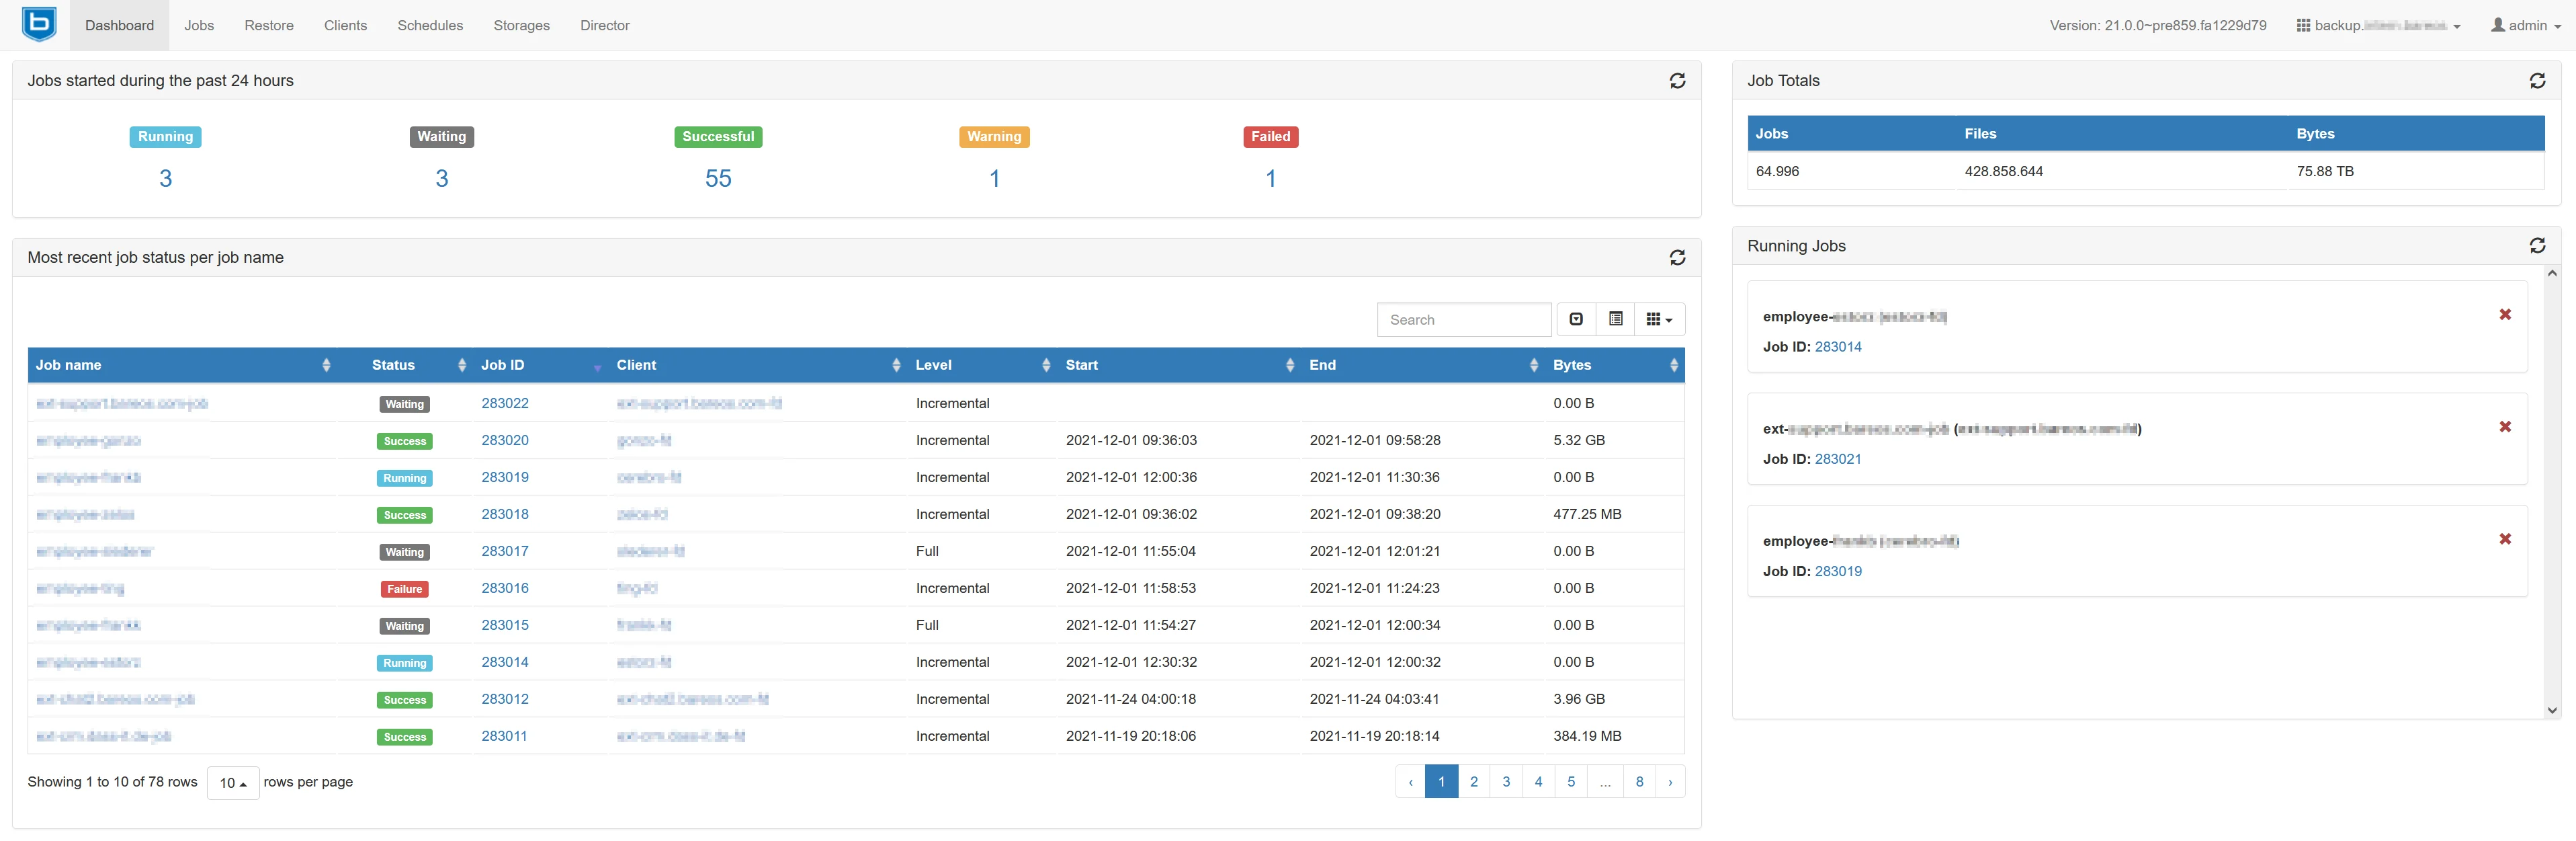
\includegraphics[width=150mm, keepaspectratio]{figures/bareos-dashboard.png}
%	\caption{A Bareos biztonsági mentéseket végző program webes felületének részlete. Forrás: \url{https://www.bareos.com/bareos-webui-modules/}}
%	\label{fig:bareos}
%\end{figure}

\section{Nagyvállalati és végfelhasználói környezetek összehasonlítása}
A legtöbb hétköznapi felhasználó számára ismeretlen vagy meglepő lehet, hogy maga az internet és az ezen keresztül elérhető szolgáltatások -- gondoljunk például az Ügyfélkapura vagy az internetbank-szolgáltatásokra -- nagyon bonyolult rendszerek nem csak szoftveres, hanem informatikai infrastruktúra szempontjából is. A legtöbb ilyen szolgáltatás egy adatközpontban lévő szerveren fut, ami a beérkező kérésekre ad válaszokat, a felhasználók az adott szolgáltató számítógépeivel kommunikálnak.

Ezek a szervergépek több lényeges különbséggel is bírnak a személyi számítógépekkel szemben. Egyik legfontosabb tulajdonságuk, hogy hibatűrőek bizonyos hardverhibákat illetően: szinte minden főbb komponensből legalább kettő áll rendelkezésre, így ha az egyik meg is hibásodik, akkor a hiba elhárításáig a beépített redundancia miatt a gép képes tovább működni, általában a felhasználók felé észrevétlenül, míg a gép üzemeltetői figyelmeztetést kapnak a hiba típusáról és a kapcsolódó tennivalókról.
% TODO: kép redundáns dolgokról (pl. hálózati kártya, PSU), és hibajelző elemekről (pl. CPU fault, RAM-hiba, diszk hiba)

A nagyvállalati informatikai környezetek számos további dologban különböznek a végfelhasználói megoldásoktól. Míg egy átlagos hétköznapi felhasználó legfeljebb két-három számítógépet, esetleg nyomtatókat és hálózati eszközöket használ tevékenységeihez, addig a nagyvállalati rendszerek sokkal nagyobb eszközparkkal dolgoznak és sokkal több felhasználó kiszolgálását biztosítják. A 24/7-es rendelkezésre állásra tervezett hardverek mellett megfigyelhetünk számos olyan megoldást, melyekkel az otthoni felhasználók nem találkoznak. Ilyenek például a fent említett szervergépek, a különböző adattárolási rendszerek és a magasabb szintű hálózati megoldások (pl.~VLAN-ok). További különbség még, hogy egyéni felhasználás esetén egy számítógépet általában csak egy-egy személy, esetleg egy család tagjai használnak, míg egy komplex szervezeti infrastruktúrát az azt üzemeltető szakemberek mellett a vállalat munkatársai és néha az ügyfelei is használják.

A nagyvállalati rendszerek a magas rendelkezésreállás biztosítása és a hibalehetőségek minimalizálása érdekében gyakran földrajzilag elkülönítetten, georedundánsan futnak, ezzel szemben egy kisebb léptékű infrastruktúra részei szinte kizárólag egy adott helyszínen találhatóak. A nagyvállalati rendszerek további ismertetőjele, hogy rendszeres és gyakori karbantartási időablakok szerint történik a hardveres és szoftveres komponensek naprakészen tartása, míg egy végfelhasználói rendszer szoftveres karbantartását gyakran maga a szoftver határozza meg, hardveres karbantartás pedig sokszor csak hiba esetén történik.

Láthatjuk, hogy az összetett infrastruktúrák üzemeltetése szakértelmet, tervezést igényel, ezáltal az üzemeltetéshez tartozó költségek is magasabbak. Ezen rendszerek karbantartása előre meghatározott ütemben, professzionális szinten történik. Kisebb infrastruktúrák és végfelhasználói megoldások karbantartása gyakran ad-hoc módon, a felhasználók megítélése alapján megy végbe. Dolgozatomban a továbbiakban a nagyvállalati rendszerek sajátosságait és a kapcsolódó üzemeltetési feladatokat ismertetem részletesen.


% !TeX encoding = UTF-8
% !TeX spellcheck = hu_HU

\chapter{Technológiai áttekintés}
\label{chap:technologies}

\section{Szervergépek}
\label{sect:servers}
A szerverek esetében jelentkező, egyénitől nagyban különböző felhasználási körülmények a~szerverszámítógépek esetén hardveres szempontból is más felépítést igényelnek. A magas rendelkezésre állás (\acrlong{ha}, \acrshort{ha}) és a modularitás, valamint az ezzel járó könnyű javítások támogatása érdekében az ilyen célra kialakított számítógépek főbb komponensei redundánsak, azaz egy-egy ilyen komponens kiesése nem jelent szolgáltatáskiesést. A~meghibásodást a rendszer egyértelműen jelzi magán a gépházon is (általában hibajelző LED-ek segítségével), valamint a menedzsment portjain\footnote{A szervergépek egy különleges interfésze, amely lehetővé teszi a számítógép távoli kezelését és a szerver által karbantartott naplók böngészését.} is. A legtöbb ilyen gép ugyanis rendelkezik egy beágyazott rendszerrel, ami lehetővé teszi a távoli kezelésüket egy webes felületen és távoli parancssori elérésen, \acrshort{ssh}-n keresztül még akkor is, ha a szervergép ki van kapcsolva. Ezek lehetőséget biztosítanak a gép legfontosabb mérőszámainak követésére, virtuális kijelző csatlakoztatására, telepítőkészletek felcsatolására, valamint a gép ki- és bekapcsolására.

\begin{figure}[!ht]
	\centering
	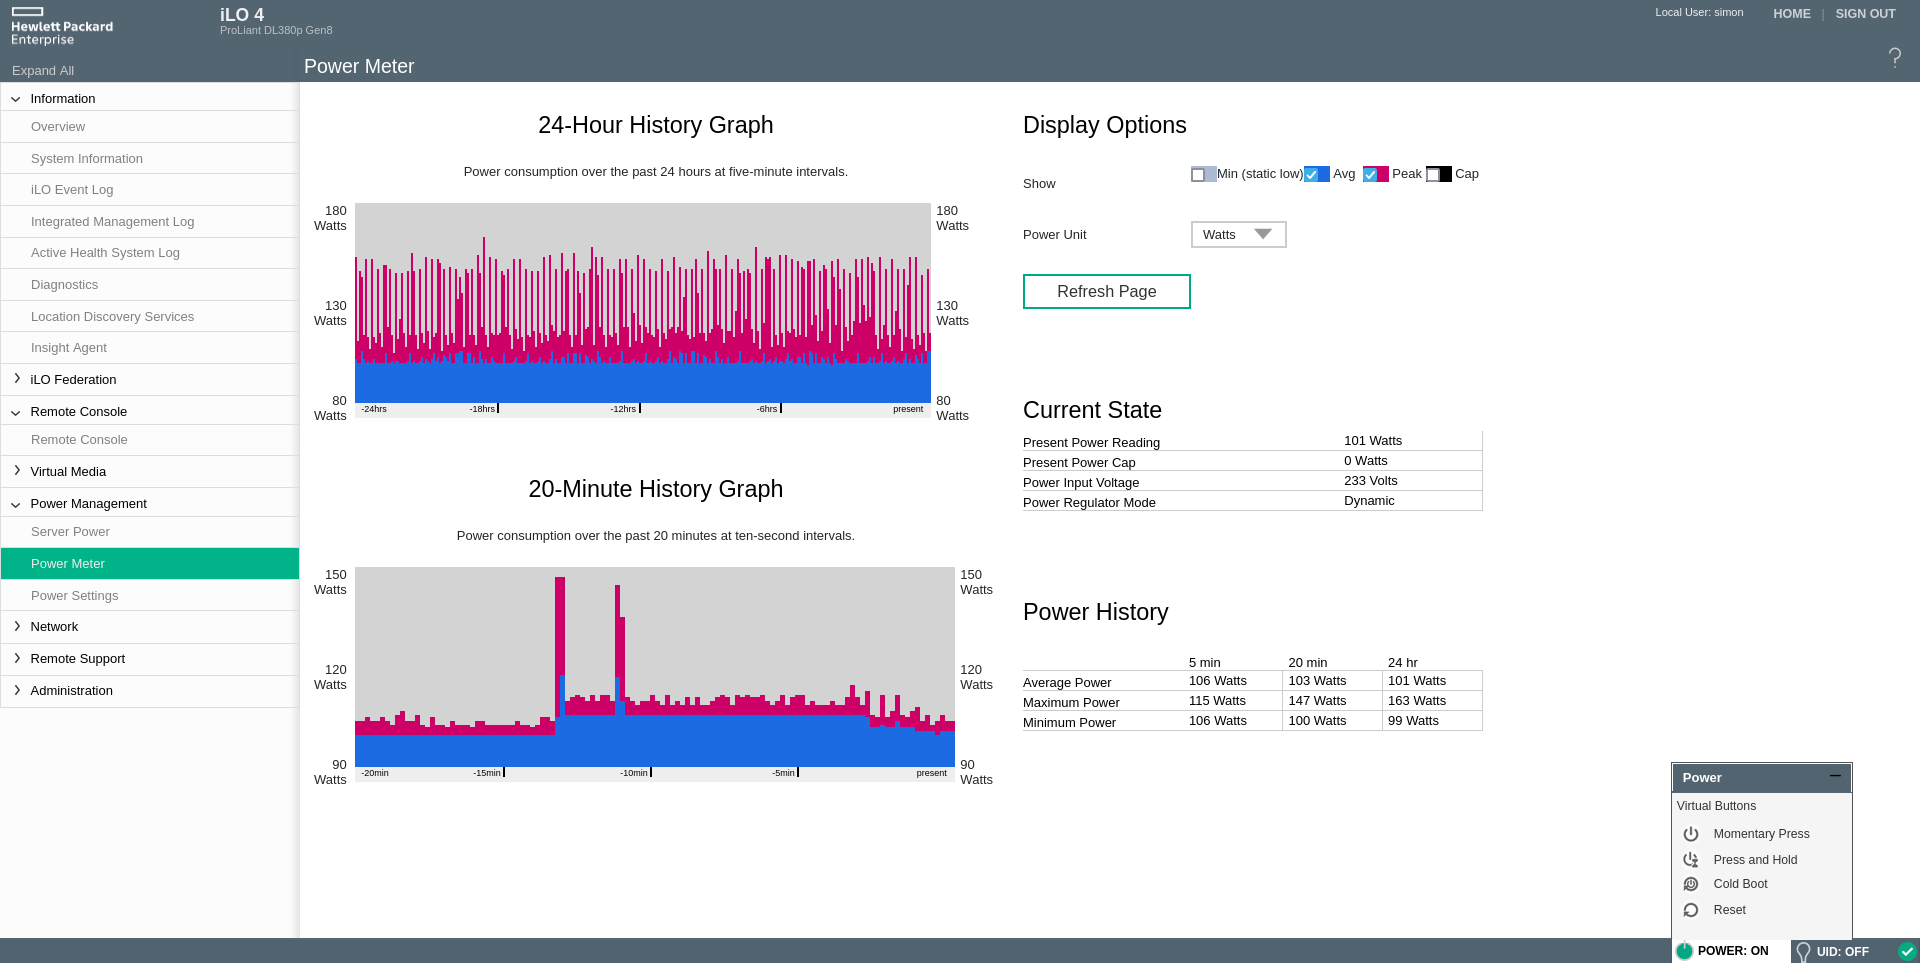
\includegraphics[width=150mm, keepaspectratio]{figures/ilo-power1.png}
	\caption{Szervergép fogyasztásának grafikonja egy HPE számítógép távoli menedzsment felületén. A jobb alsó sarokban megjelenő menüvel lehetőségünk van a gép kikapcsolására és újraindítására is.}
	\label{fig:ilopowerchart}
\end{figure}

A fent ismertetett üzemeltetést, karbantartást könnyítő felépítés mellett általában elmondható, hogy az ilyen gépek jelentős része virtualizációra van tervezve -- persze ezektől különböző felhasználási módok is jelentkeznek (például fájlszerverek tervezése során a teljesítmény helyett a minél nagyobb tárkapacitásra és adatátvitelre helyezték a hangsúlyt). A dolgozat szempontjából viszont a nagyvállalati környezetben domináló virtualizációs felhasználási terület lesz a lényegesebb, így a továbbiakban az ilyen számítógépekre (virtualizációs hoszt, virtualization host) koncentrálok.

A virtualizációs hosztgépek jellemzője, hogy számos processzorral rendelkeznek, valamint felhasználói szemmel szokatlanul nagy memóriaterülettel bírnak. Ki fog derülni azonban, hogy 12-24 processzormag és akár több száz gigabyte memória is szűkös erőforrássá válhat egy virtuális gépeket futtató számítógép esetében, hiszen gyakorlatilag itt egyetlen szervernek kell elbírnia akár több tíz számítógép terhelésével is. Ezek mellett általában több (8-24) háttértár-foglalattal is rendelkeznek, melyekhez hardveres RAID-támogatást is adnak. A RAID-megoldásokkal \aref{sect:raid}.~alfejezet foglalkozik részletesebben.

\section{Virtualizáció}
A fent említett megnövekedett forgalom kiszolgálását hatékonyan lehet kezelni úgy, hogy olyan fizikai számítógépet helyezünk üzembe, mely  több, egymástól független operációs rendszer futtatására is alkalmas. Ilyenkor ezeket a fizikai gépen futó rendszereket virtuális gépeknek (\acrlong{vm}, \acrshort{vm}) nevezzük. Egy virtuális gép elkülönített erőforrásokat kap a fizikai géptől, hozzáférhet például bizonyos mennyiségű processzormaghoz, memóriához, illetve külön háttértár-partíciói is lehetnek. A virtualizált hardverek és operációs rendszerek a legtöbb esetben a külvilág felé nem különböztethetőek meg a fizikai számítógépektől, és ezzel a megoldással jelentősen csökkenthető a rendszerek és a hozzájuk szükséges informatikai infrastruktúra üzemeltetésének költsége.

A virtualizáció nagy ereje abban rejlik, hogy bizonyos hardverek virtualizációjával egységnyi teljesítményt olcsóbban kaphatunk meg, mintha külön fizikai gépeket helyeznénk üzembe, illetve nagyobb rugalmasságot kapunk a kezelésükben, üzemeltetésükben. Képzeljük el, hogy megveszünk egy számítógépet, amin szeretnénk futtatni egy számunkra fontos alkalmazást, mondjuk a honlapunkat. Ilyenkor az ezen a gépen futó operációs rendszer teljes mértékben megszabhatja, hogy milyen erőforrásokból mennyit használ. Ha~egy másik szolgáltatást -- például levelezőszervert -- szeretnénk emellett futtatni, akkor korlátozottabbak a lehetőségeink, hiszen a korábban telepített webszerver már foglal bizonyos erőforrásokat, illetve a program függőségeit és konfigurációs fájljait is telepítettük már, ami esetleg negatívan hat a levelezőszerverünk működésére. Ha mindezt virtualizált környezetben tesszük meg, akkor a topológia megváltozik: a két alkalmazás teljesen elkülönítetten, egymás zavarása nélkül, különböző virtuális gépeken futhat, ezeket a gépeket pedig a fizikai gépen futó egyik szoftverkomponens, az úgynevezett \gls{hypervisor} kezeli, mely a gazdagépen futó rendszer legfőbb virtualizációt támogató komponense~\cite{Sles15virt}. A \gls{hypervisor} látja el az erőforrások ütemezésének és kiosztásának (pl.~processzoridő, memória) feladatát, gondoskodik a virtuális gépek számára szükséges hardveres erőforrások virtualizált hardverinterfészeken keresztüli elérhetőségéről.
% TODO: virt-manager screenshot, esetleg virsh xml screenshot

\subsection{Népszerű virtualizációs technológiák}
Mivel a virtualizáció nagyon elterjedt technológia, számos olyan megoldás született, mely egyszerűsíti a virtuális gépek üzemeltetését. Ezek közül nagy ismertségnek örvend az Oracle~VirtualBox és a VMware~Player, azonban ezek a megoldások nem skálázódnak annyira jól, mint a továbbiakban tárgyalt társaik, melyek sokkal megfelelőbbek nagyvállalati szerverkörnyezetben való alkalmazásra. Ezek a \gls{hypervisor}ok lehetőséget biztosítanak a virtuális gépek távoli elérésre, kezelésére, egyszerűbb telepítésükre, valamint szükség esetén elosztott működésükre. A következőkben három népszerű virtualizációs technológiát fogok bemutatni, összehasonlításuk \aref{tab:hypervisor-comparison}.~táblázaton látható.

A \gls{hypervisor}okat két kategóriába sorolhatjuk Robert P. Goldberg 1973-as publikációja alapján~\cite{Goldberg1973Hypervisors}. Az egyes típusú hypervisorok \mbox{(type-1)} natívan, közvetlenül a gazdagépen futnak (pl.~a következőkben tárgyalt VMware~ESXi), míg a kettes típusba tartozó \mbox{(type-2)}, úgynevezett hosztolt hypervisorok egy hagyományos operációs rendszeren futnak más számítógépes programokhoz hasonlóan. Kettes típusú hypervisor például az Oracle~\mbox{VirtualBox}. Egyes hypervisorok --~mint a~későbbiekben ismertetett \acrshort{kvm}~-- besorolása vitatott, mivel egy kernelmodulként épül bele egy már futó \acrshort{os}-be. Azonban mivel azt így lényegében egy type-1 \gls{hypervisor}rá alakítja, ezért általában az egyes típusba sorolják~\cite{WikiHypervisor}. A két típus felépítését \aref{fig:hypervisors}.~ábra mutatja be.

\begin{figure}[ht]
	\centering
	\begin{tikzpicture}[node distance=1.4cm]
	\definecolor{midnightblue}{HTML}{192072}
	\definecolor{junglegreen}{HTML}{30BA78}
	\definecolor{waterholeblue}{HTML}{2453FF}
	\definecolor{persimmon}{HTML}{FE7C3F}

	\tikzstyle{rect} = [rectangle, rounded corners, draw=midnightblue, minimum width=4.6cm, minimum height=1.2cm, text centered, text=black, font=\fontsize{12}{12}\selectfont, line width=1.25pt]
	\tikzstyle{vm-rect} = [rectangle, rounded corners, draw, minimum width= 2.2cm, minimum height=1.2cm, text centered, font=\fontsize{12}{12}\selectfont, line width=1.25pt]
	
	\node (hardware) [rect] {Fizikai gép};
	\node (hypervisor) [rect, above of = hardware, draw=junglegreen] {Hypervisor};
	\node (vm1) [vm-rect, above of = hypervisor, xshift=-1.2cm, draw=persimmon] {VM};
	\node (vm2) [vm-rect, above of = hypervisor, xshift=1.2cm, draw=persimmon] {VM};

	\node (hardware2) [rect, right of = hardware, xshift=5cm] {Fizikai gép};
	\node (os) [rect, above of = hardware2, draw=waterholeblue] {Operációs rendszer};
	\node (hypervisor2) [rect, above of = os, draw=junglegreen] {Hypervisor};
	\node (vm1_2) [vm-rect, above of = hypervisor2, xshift=-1.2cm, draw=persimmon] {VM};
	\node (vm2_2) [vm-rect, above of = hypervisor2, xshift=1.2cm, draw=persimmon] {VM};

\end{tikzpicture}

	\caption{Type-1 és type-2 \gls{hypervisor}ok felépítése.}
	\label{fig:hypervisors}
\end{figure}

Nagyvállalati környezetben elterjedt virtualizációs megoldás például a VMware~ESXi, amely egy igen modern \gls{hypervisor} számos kényelmi funkcióval ellátva (lehetőség van például a rendszer webes felületről való kezelésére és virtuális gépek sablonból való gyors, körülbelül 5-10 perc alatti telepítésére). Az ESXi a részletes beállításokat lehetővé tevő, könnyen kezelhető webes felületének köszönhetően nagy piaci részesedést szerzett, felmérések alapján kb. 60-80\%-os jelenléttel uralja a virtualizációs piacot, bár a közelmúltban bevezetett új, jelentősen drágább előfizetési modell némileg csökkenthet ezen az~arányon~\cite{VmwareMarketshare}~\cite{VmwareCustomerDecline}.
Egy~másik kedvelt megoldás az ESXi-vel ellentétben felhasználási korlátozás nélkül teljesen ingyenesen, GPLv2-es licenc alatt elérhető XEN~\gls{hypervisor}. Ez~ugyan kevesebb kényelmi funkciót tartalmaz, de szintén népszerűségnek örvend széleskörű támogatása, kedvező teljesítménye és szabad szoftver voltából eredő ingyenessége miatt. A XEN a 2014~márciusában kiadott 4.4-es~verzió óta stabilan működik együtt a \gls{libvirt} virtualizációs \acrshort{api}-val, amely nagyban megkönnyíti a \gls{hypervisor}ral való kommunikációt a virtuális gépek konfigurálása során~\cite{Xen44ReleaseNotes}.

A XEN-hez hasonlóan szabadszoftver-licenccel érhető el a \acrfull{kvm} is, mely a XEN-nél modernebb megoldásnak tekinthető, és manapság széles körben használják a Linux kernelbe való integráltságának és stabilitásának köszönhetően. Bár maga a \acrshort{kvm} nem tartalmaz ilyet, de számos interfész elérhető az ezen keresztül futtatott virtuális gépek kezelésére (például~virt-manager és további, a XEN-nél említett \gls{libvirt} \acrshort{api}-t támogató  szoftverek), valamint akadnak olyan megoldások is, melyek a \acrshort{kvm}-re alapozva nyújtanak szélesebb körű virtualizációs megoldást, ilyen lehet\footnote{A konfigurációtól függően akár többfajta virtualizációs környezet is beállítható, de a \acrshort{kvm} az egyik legjobban támogatott.} például a Proxmox és a Cockpit.

\begin{table}[h!]
	\setlength{\tabcolsep}{5pt}
	\renewcommand{\arraystretch}{1.3}
	\centering
	\begin{tabular}{||p{3.25cm} p{3.25cm} p{3.25cm} p{3.25cm} ||}
		\hline
		Megnevezés & VMware ESXi & XEN & KVM \\
		\hline\hline
		Fejlesztő & VMware LLC & Linux Foundation, Intel & Linux fejlesztői közösség \\
		\hline
		Licencelés & zárt forráskódú, korlátozott ingyenes verzió, teljes verzióhoz előfizetés szükséges & szabadon hozzáférhető, GPL & szabadon hozzáférhető, GPL \\
		\hline
		Támogatott architektúrák & x86-64, ARM & IA-32, x86-64, ARM & ARM, PowerPC, ESA/390, IA-32, x86-64 \\
		\hline
		\Gls{hypervisor} típusa & Type-1 & Type-1 & Type-1 \\
		\hline
		Hivatalosan támogatott \acrshort{vm} \acrshort{os}-ek & Linux, BSD, Windows, macOS & Linux, BSD, Windows, macOS & Linux, BSD, Windows, macOS \\
		\hline
		Aktív \gls{libvirt} támogatottság & Limitált & Igen & Igen \\
		\hline
		Támogatás & Hivatalos & Közösségi & Közösségi  \\
		\hline
		\acrshort{cpu} \gls{hotswap} & Igen & Igen & Igen \\
		\hline
		Memória \gls{hotswap} & Igen & Igen & Igen \\
		\hline
		Megjegyzés & Könnyű kezelhetőségének, jó támogatásának köszönhetően napjaink legelterjedtebb virtualizációs platformja. A~másik két Linux-közeli megoldáshoz képest kevesebb illesztőprogram áll rendelkezésre, így szigorúbb hardveres követelményeket támaszt. & Eredetileg egyetemi projektként indult, a 2000-es évek közepén nagy fejlődésen ment keresztül, számos nagy platform (pl.~Amazon~AWS) építette XEN-re a virtualizációs technológiáját. & Hivatalosan is a Linux kernel része, így folyamatos fejlesztés alatt áll és hatékonyan együtt tud működni a kernellel. Számos virtualizációs platform (pl.~Google Cloud Platform) alapjaként szolgál.  \\
		\hline
	\end{tabular}
	\caption{A tárgyalt virtualizációs megoldások összehasonlítása.}
	\label{tab:hypervisor-comparison}
\end{table}


\subsection{Virtuális gépek használatának néhány előnye}
A virtualizáció számos előnnyel járhat az infrastruktúra és a kiszolgálni kívánt alkalmazások szempontjából. Az egyik legnagyobb ilyen előny például, hogy a virtuális gépek egymástól izoláltan futnak, azaz nincs közvetlen kapcsolat közöttük, ami biztonsági és kezelési, tesztelési szempontból is kedvező lehet. Egy adott csomag vagy szoftver kipróbálásához például készíthetünk egy teszt virtuális gépet, amit egyszerűen törölhetünk a~teszt végeztével --~a telepített program eltávolítása hagyományos környezetben futtatva sokkal körülményesebb lenne. Hasonlóan előnyökkel jár, hogy a legtöbb modern \gls{hypervisor} lehetőséget biztosít bizonyos erőforrások úgynevezett \textit{\gls{hotswap}}elésére. Ez azt jelenti, hogy egyes komponenseket (pl.~memória, háttértárak) úgy is kicserélhetünk, hogy a rendszert nem szükséges ehhez leállítanunk, így a karbantartás nem jár szolgáltatáskieséssel. A felsoroltakon túl a virtuális gépek néhány további kedvező tulajdonságát ismertetem részletesen a következő alfejezetekben.

\subsubsection{Erőforrások testreszabása}
Amikor több tíz vagy több száz szerver üzemeltetéséről van szó, akkor hatványozottan számításba kell vennünk az egyes gépekre jutó költségeket. Virtuális gépek esetén ez azért kedvezőbb egy fizikai gépnél, mert ugyan a nagyvállalati környezetbe szánt szervergépek jelentősen drágábbak a személyes felhasználásra tervezett társaiknál, de akár több tíz virtuális gép egyidejű futtatását is lehetővé teszik. Ezáltal az egy fizikai gépre eső, asztali gépeknél megszokott áramfogyasztáshoz képest jóval nagyobb energiafelvétel sokkal kedvezőbb arányt mutat, ha számításba vesszük a futtatott virtuális kiszolgálók számát is.

Mindezek mellett a nagyvállalati felhasználáshoz tervezett számítógépek jóval hibatűrőbbek, hiszen a főbb komponensek redundánsan lettek kialakítva: ezekből az ilyen szerverekben legalább kettő van, és a rendszer automatikusan képes detektálni a hardveres hibákat, és ezek figyelembe vételével tovább működni.

Előnyös lehet továbbá, hogy a virtuális gépek erőforrásai szabadon módosíthatók, így akár két újraindítás között is változtathatjuk a rendelkezésre álló memória mennyiségét vagy épp a processzormagok számát. Sőt, egyes \gls{hypervisor}ok és operációs rendszerek ezen erőforrások futásidejű megváltoztatását is támogatják bizonyos korlátozások mellett, így gyakorlatilag a fontosabb virtualizált erőforrások is \gls{hotswap}elhetőnek tekinthetőek.

\subsubsection{Pillanatképek}
Egy másik kedvező lehetőség virtuális gépek használata esetén az, hogy pillanatképeket, úgynevezett snapshotokat készíthetünk róluk. Ezek a gépet egy adott pillanatbeli állapotban reprezentálják, és később ezeket visszaállíthatjuk, ha szükségünk lesz rá. Egyes megoldások a memóriakép mentését is támogatják, így akár egy futó gép is könnyen visszaállítható. A pillanatképek készítése hasznos lehet például rendszerfrissítések esetén, így ha valamiféle hiba lép fel a frissítés során, vagy egy adott szoftver nem megfelelően működik azt követően, akkor a frissítés előtt készített snapshotra visszaállva újra teljes értékűen üzemelhet a szerver, amíg a frissítés során fellépő hibát el nem hárítjuk.

\subsubsection{Migráció}
Részben az előző ponthoz kapcsolódik a virtuális gépek migrációja. Ez a funkció azt jelenti, hogy egy adott fizikai gépről, mely virtuális gépeket futtat (virtual host), készíthetünk egy snapshotot, amit áthelyezhetünk egy másik virtual hostra, és a virtuális gép ezen futhat tovább egyéb újrakonfigurálás nélkül.
Lehetőség van azonban a háttértárak tartalmát elhagyva is átmozgatni egy VM-et egy másik hosztra. Ehhez bevett szokás leírófájlok használata, mely egy virtuális gép konfigurációját tartalmazza. A leírófájlt egy másik hosztgépre áthelyezve ott újra elindíthatjuk a definiált virtuális gépet. Ilyenkor szükség lehet a~\acrshort{vm} háttértárainak inicializálására, de ettől eltekintve a konfiguráció szabadon hordozható virtual host-ok között. Ilyen migrációra egyes megoldások fejlettebb támogatást is adnak, így akár valós időben, az aktuális terheltség figyelembe vétele mellett automatikusan is áthelyezhetőek virtuális gépek a megadott fizikai hosztok között.
% TODO: listing egy példa virsh xml-lel

\subsection{Konténerizáció}
A konténerizáció a virtuális gépekétől némileg különböző megoldást használ a szolgáltatások elkülönített futtatására. A motiváció hasonló: egy-egy alkalmazást szeretnénk a gazdagéptől elkülönítetten üzemeltetni. Felmerült azonban az igény, hogy a virtuális gépekhez képest kisebb költsége legyen a szolgáltatások futtatásának. Ezt úgy lehetett csökkenteni, hogy egy teljes virtuális gép létrehozása helyett csak egy minimális izolált környezetet hozunk létre, amely tartalmazza az alkalmazás működéséhez szükséges fájlokat, függőségeit. Az így létrejövő környezeteket konténereknek nevezzük. Egy-egy konténer egyszerűen mozgatható kiszolgálók között, és az adott alkalmazás függőségei egységbe zárásának köszönhetően a gazda operációs rendszertől függetlenül szinte bármilyen \acrshort{os}-en futtatható. A technológia egyre nagyobb teret hódít meg, a népszerű konténerizációs megoldások közé tartozik a Docker, a Podman és a témához szorosan kapcsolódik a népszerű konténer-orkesztrációs platform, a Kubernetes is. Bár a következőkben tárgyalt fejezetekben lesz szó a konténerizációról, és a tesztkörnyezetben egy konténerhoszt-\acrshort{vm}-et is telepítettem, melyben hoztam létre konténert, magára a technológia alkalmazására az itt ismertetettnél nem térek ki részletesebben.

\section{RAID}
\label{sect:raid}
Nagyvállalati környezetben nem hagyhatjuk ki a~\acrfull{raid} megoldásokat (a népszerű \acrshort{raid}~1-et és \acrshort{raid}~6-ot \aref{fig:raid}.~ábra szemlélteti), ha~biztonsági mentésről beszélünk. Ezek arra adnak lehetőséget, hogy az adatokat több fizikai háttértáron (pl. merevlemez vagy SSD) tároljuk úgy, hogy egy esetleges lemezhiba ne~okozzon fennakadást a működésben. Fontos tisztában lenni azonban azzal, hogy a~\acrshort{raid}-megoldások nem védenek bizonyos veszélyek ellen (például zsarolóvírusok, fájlok korruptálódása), hiszen az adatok duplikálása valós időben történik, így egy esetleges támadás során a \acrshort{raid}~poolba\footnote{\acrshort{raid}~poolnak nevezzük azon fizikai kötetek összességét, amelyek együtt egy \acrshort{raid}-kötetet adnak, például \aref{fig:raid}.~ábrán a \acrshort{raid}~1 és \acrshort{raid}~6 kötetet adó háttértárak egy-egy \acrshort{raid}~poolt alkotnak.} bevont összes diszken megváltoznak az adatok, így nem alkalmas a támadás utáni visszaállításra. Emiatt egy \acrshort{raid}~pool \aref{sect:datasec}.~alfejezetben részletezett \textit{3-2-1} mentési stratégiát alkalmazva csak egyetlen eszköznek tekinthető, hiába több lemezt használunk a mentés során. \acrshort{raid}-elést tehát csak hardveres hibák ellen érdemes használnunk, rosszindulatú támadás esetén ezek nem nyújtanak védelmet az adataink számára.

% TODO: RAID ábra, hivatkozások
\begin{figure}[!ht]
	\centering
	\begin{subfigure}{0.3\textwidth}
		\centering
		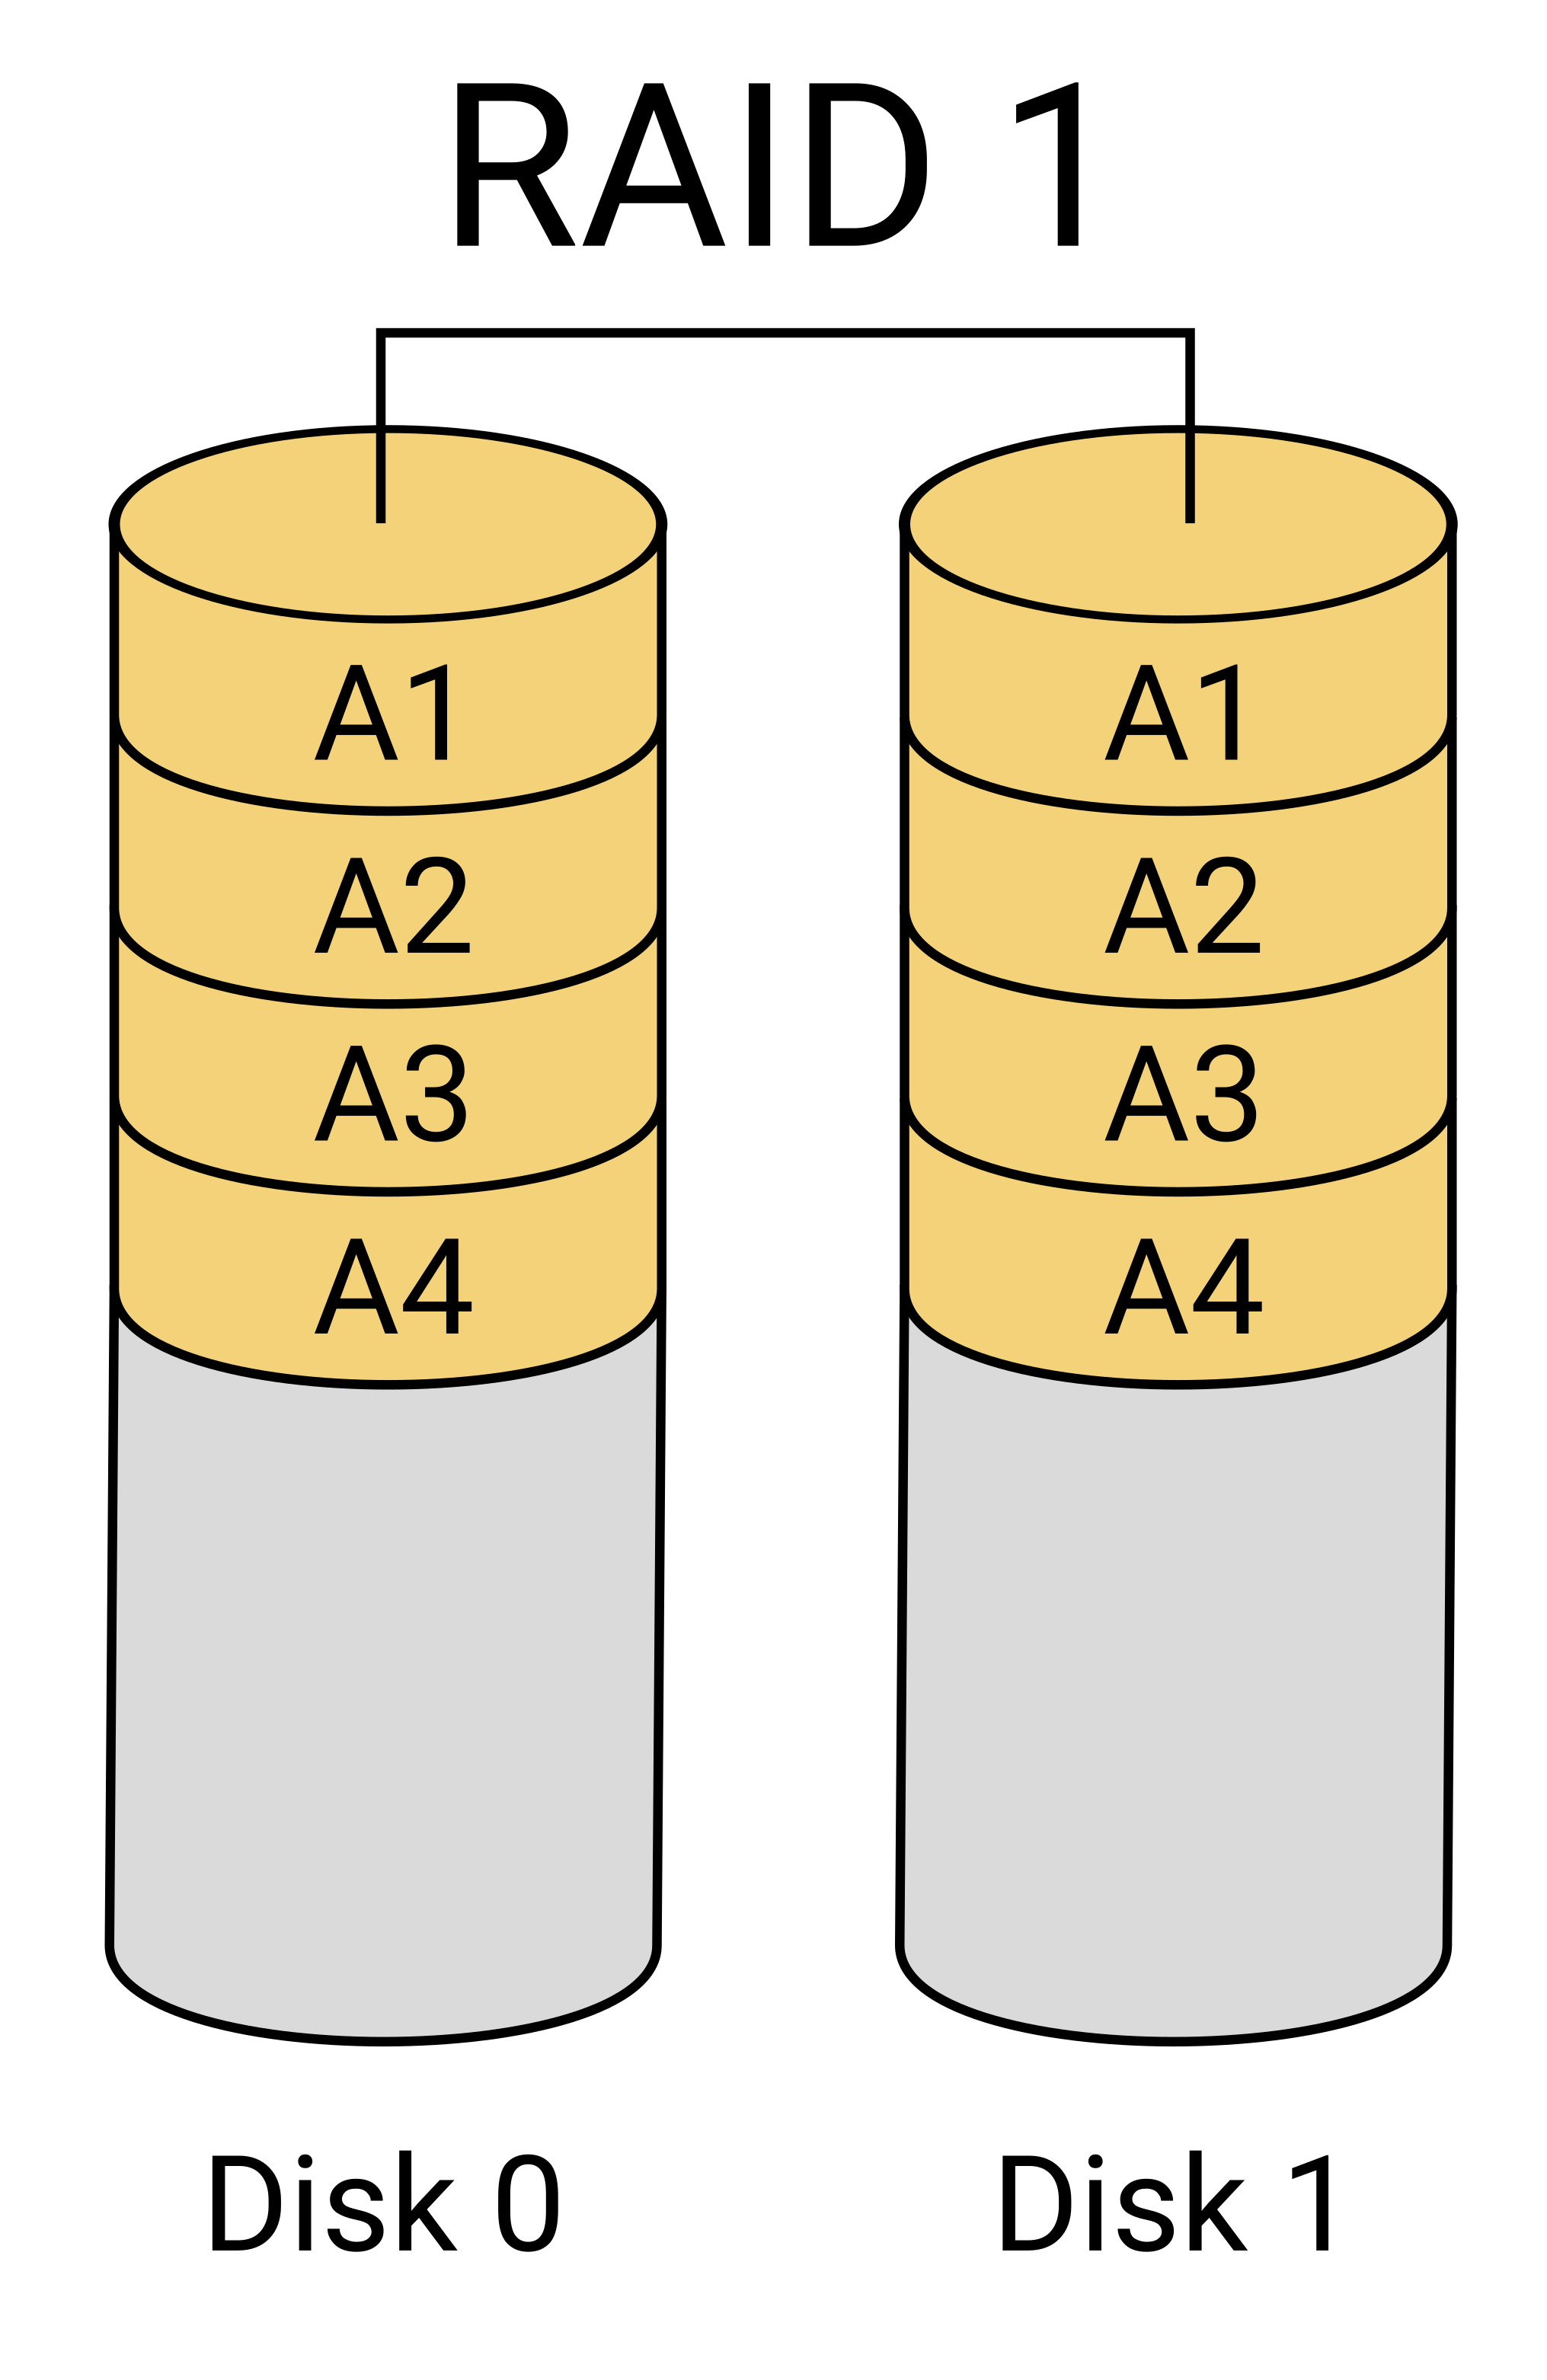
\includegraphics[keepaspectratio, height=52mm]{figures/raid1.pdf}
	\end{subfigure}
	\hspace{0.05\textwidth}
	\begin{subfigure}{0.6\textwidth}
		\centering
		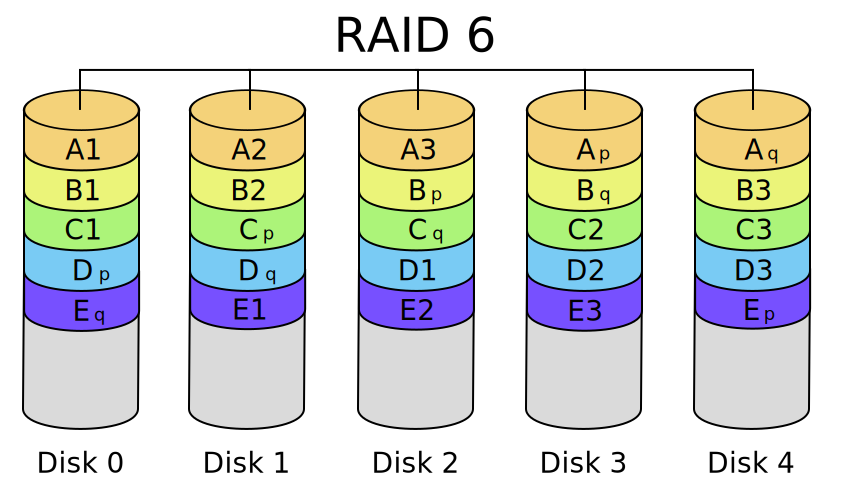
\includegraphics[keepaspectratio, height=52mm]{figures/raid6.pdf}
	\end{subfigure}
	\caption{\acrshort{raid} 1 és \acrshort{raid} 6 megoldások felépítése \cite{WikiRaidLevels}.}
	\label{fig:raid}
\end{figure}


\section{Logikai kötetkezelés}
\label{sect:lvm}
Mind a fizikai, mind a virtuális gépek esetén szükség lehet háttértárakra az adatok perzisztens tárolása érdekében. Hagyományos particionálási megoldásokkal hamar nehezen kezelhetővé válhatnak a különböző csatolási pontok\footnote{Unix-alapú operációs rendszerekben azokat a könyvtárakat nevezzük csatolási pontoknak, amelyeken keresztül elérhetjük az adathordozók, lemezképfájlok tartalmát.} és a virtuális gépek számára kiosztott kötetek. Az ilyen problémák elkerülésére jött létre a logikai kötetkezelés, mely a tárhely-virtualizáció egy formája. A logikai kötetkezelésnek több implementációja létezik, ezek közül jelenleg a Linux kernelben elérhető \gls{lvm}-et ismertetem részletesen.

A Linux logikai kötetkezelője három lényegi rétegből áll: a fizikai kötetből (\acrlong{pv}, \acrshort{pv}), a kötetcsoportból (\acrlong{vg}, \acrshort{vg}) és a logikai kötetekből (\acrlong{lv}, \acrshort{lv}). Ezt a felépítést \aref{fig:lvm}.~ábra szemlélteti egy egyszerű \gls{lvm}-konfiguráción keresztül.
Lehetőség van ennél összetettebb kötetkiosztás létrehozására is, például egy kötetcsoport több fizikai kötetből is állhat, amik akár külön háttértáron is lehetnek, sőt, \acrshort{raid}-csoportot is megadhatunk egy \gls{lvm}-partíció alapjául. Ezen megoldások használata azonban sok hátránnyal járhat (pl. diszkhiba esetén nehezebb visszaállítani a partíciót), ezért ennek használata alapvetően nem ajánlott~\cite{RHLVM}.

\begin{figure}[!ht]
	\centering
	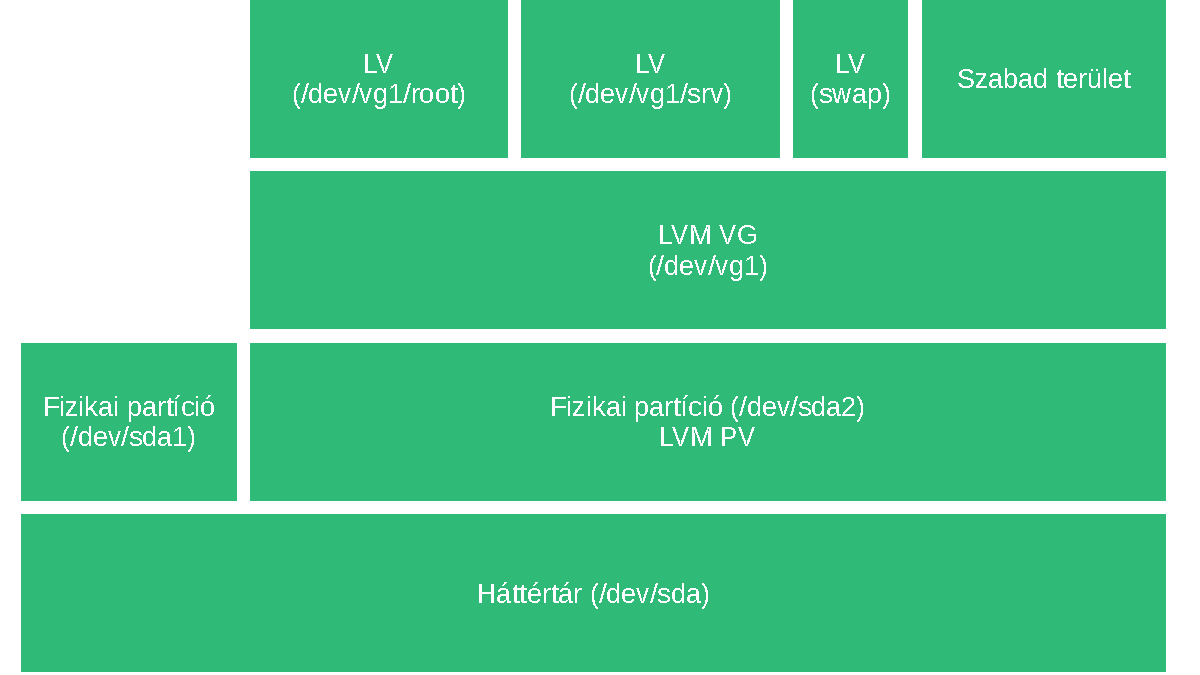
\includegraphics[width=14cm]{figures/lvm.pdf}
	\caption{Egyszerű \acrshort{lvm}-kötetkezelési hierarchia.}
	\label{fig:lvm}
\end{figure}

Az \gls{lvm} tehát úgy épül fel, hogy egy vagy több háttértáron létrehozunk hagyományos fizikai partíciókat, melyek az \gls{lvm} \acrshort{pv}-k alapjául fognak szolgálni. Ezt követően létrehozzuk a kötetcsoportokat az általuk használandó \acrshort{lvm} fizikai kötetek megadásával. Az így létrejött csoportban már tudunk létrehozni logikai köteteket, amíg van szabad hely a \acrshort{vg}-ben.

Láthatjuk, hogy az \acrshort{lvm}-kötetek használata kezdetben több feladattal jár, mint a~hagyományos partíciók esetében, azonban hosszabb távon számos előnnyel jár. Talán a~logikai kötetkezelés legnagyobb előnye, hogy szabadon foglalhatunk le tárterületet a létrehozott köteteknek: ha azt tapasztaljuk, hogy az egyik köteten kevés a szabad hely, akkor fájlrendszertől függően elég lehet akár egy parancs kiadása is ennek kiterjesztéséhez. Lényeges, hogy a hagyományos partíciók használatával ellentétben a logikai kötetkezelés használatakor figyelmen kívül hagyhatjuk a partíciók elhelyezkedésének sorrendjét, így nem szükséges figyelembe vennünk, hogy az adott partíció előtt vagy után van-e szabad tárterület. A~megnövelt kötet helyes fizikai háttértárra képzéséről a logikai kötetkezelő fog gondoskodni számunkra. Fontos megjegyezni, hogy a kötetbővítés online is elvégezhető, azaz nem szükséges a kötetet lecsatolni a gépről az átméretezéshez. Ez különösen fontos lehet például a fájlrendszer gyökerét jelentő root~(/) partíció növelése során, hiszen ezt csak a számítógép leállítása mellett tudjuk biztonságosan lecsatolni. Előállhat olyan helyzet is, hogy egy~másik (nem root) partíciót kell online átméreteznünk, például ha azt tapasztaljuk, hogy egy adatbázisszerveren hirtelen nagy mértékben nőtt a tárolt adat mérete. Ilyenkor~nincs lehetőség a szerver leállítására, hiszen ez esetben az alkalmazások nem tudnák használni az adatbázist a leállás idejére. Az ehhez hasonló helyzetekre is jó megoldást nyújt a logikai kötetkezelő egy megfelelő, online átméretezést támogató fájlrendszer (pl. XFS, Btrfs) használata mellett. Érdemes megjegyezni, hogy bár az \acrshort{lvm} és például a Btrfs-fájlrendszer nyújt támogatást a növelésen kívül a fájlrendszer méretének csökkentésére is, ez a művelet általában nem biztonságos, és adatvesztéshez vezethet. Emiatt érdemes eleinte csak kisebb tárterületet adni a köteteinknek, hiszen kiterjeszteni sokkal egyszerűbb őket, mint csökkenteni a méretüket. Ennek megkönnyítésére is ad lehetőséget az \acrshort{lvm}, megadhatjuk, hogy egy kötet egy bizonyos arányú tárhelyhasználat után automatikusan bővüljön, így elkerülve annak betelését.

Az \acrshort{lvm} hasznos funkciói közé tartozik még a kötetpillanatképek (volume snapshots) készítésének lehetősége. Ez azt jelenti, hogy a kötetkezelő képes az adott kötet adott pillanatbeli helyzetének rögzítésére, és erre a verzióra szükség szerint visszaállhatunk (rollback). Ez hasznos lehet például nagyobb konfigurációs változások eszközölése esetén, gyorsan változó adatokkal dolgozó rendszerek (pl. adatbázisszerver) biztonsági mentéseinek készítése során, illetve rendszerfrissítések előtt.\footnote{Egyes eszközök és operációs rendszerek (pl. openSUSE-verziók a snapper-rel (\url{https://doc.opensuse.org/documentation/leap/reference/html/book-reference/cha-snapper.html}) automatikusan készítenek snapshotot a frissítések telepítése előtt, így hiba esetén visszaállhatunk a frissítés előtti verzióra.}

\section{OS-lehetőségek} \label{sect:os}
Egy nagyvállalati informatikai infrastruktúrában nagy szerepe van a választott operációs rendszernek is, ugyanis nem mindegy, hogy a több száz számítógépből álló rendszerünket mennyire hatékonyan tudjuk karban tartani, egy kritikus biztonsági frissítést milyen hamar tudunk telepíteni az érintett eszközökre, és probléma vagy különleges igény esetén milyen támogatásra számíthatunk a szoftvereinket illetően.
Ezeket a szempontokat figyelembe véve manapság elsősorban a Debian, Ubuntu, Red Hat Enterprise Linux és SUSE Linux Enterprise diszribúciók közül választanak a vállalatok.

A Debian stabilitása miatt népszerű választás elsősorban kisebb (néhány tíz gépből álló) infrastruktúrák esetében, viszont a stabilitás az elérhető csomagok verzióinak rovására megy, általában a legújabbnál néhány verzióval régebbi csomagokat szállítanak a disztribúcióval. A Debian előnye, hogy teljesen szabadon elérhető, és bár nincs hozzá hivatalos támogatás, harmadik féltől vásárolhatunk ilyen szolgáltatást.

Az Ubuntu egy Debian-alapú operációs rendszer, melyet a Canonical Ltd. fejleszt, és vállalati támogatást is nyújt az OS-hez amellett, hogy az alapverzió ingyenesen érhető el. Előnye, hogy mivel mind szerver, mind pedig asztali környezetben elterjedt rendszer, számtalan projekt és gyártó adja ki a szoftvereit Ubuntu rendszerekre.

A Red Hat és a SUSE Linux-verziók már inkább egy magasabb kategóriát céloznak meg: fő célközönségük a több száz, illetve több ezer gépes környezetet üzemeltető vállalatok, és a fent említett két disztribúciónál alapesetben (a legkisebb támogatási csomagban) is szélesebb körű támogatást biztosítanak az operációs rendszerekhez. Kiemelendő, hogy ez~a~két disztribúció egyedülálló a biztonság területén: számos biztonsági tesztnek vetették alá őket különböző szervezetek (köztük például kormányzatok és IT-biztonságra specializálódott cégek is), melyeket követően a kereskedelmi forgalomban lévő Linux-disztribúciók közül a legmagasabb minősítéseket és tanúsítványokat kapták meg ezek a rendszerek~\cite{RhSec}~\cite{SlesSec}.

Lényeges különbség még, hogy az utóbbi két operációs rendszer \acrshort{rpm}-alapú csomagkezelőt használ, mely a Debian és Ubuntu által használt DEB formátumhoz képest több lehetőséget biztosít például javítások (patchek) telepítésére. Emellett ez a formátum általában jobb támogatottságot élvez vállalati szoftverek esetében, ezért ezekben a felhasználási körökben az \acrshort{rpm}-csomagokat használnak a DEB-csomagokkal szemben.


\section{Infrastruktúra-menedzsment}
Komplex infrastruktúrák esetén egyre nehezebbé válik a szerverek konfigurációjainak karbantartása, a frissítések kezelése. Manapság már széles körben elterjedtek az~infrastruktúramenedzsment-megoldások, melyek lehetőséget biztosítanak ezen problémák kiküszöbölésére. Alkalmazásukkal hatékonyabbá tehető a számítógépek szoftveres karbantartása, könnyen egységesíthetőek a konfigurációs állományok, és így egyszerűbben kezelhetővé válnak az azonos szerepű számítógépek, rendszercsoportok.

\subsection{Ansible és Salt}
Dolgozatomhoz az Ansible-t és az Uyuni alapjául szolgáló Salt-ot vizsgáltam meg közelebbről. Mindkét megoldás elterjedtnek tekinthető, azonban a felépítésük nagyban különbözik.

Az Ansible sikere az egyszerűségében rejlik: az Ansible szerveren, az úgynevezett \textit{Control Node}-on kívül nincs szükség további komponensek telepítésére az alapvető funkciók használatához. Az Ansible nem használ dedikált kliensszoftvereket, ezért \textit{agentless}-nek nevezik, működése a push modellen\footnote{A kliens-szerver kommunikációban kétféle modellt különböztetünk meg attól függően, hogy a kliens vagy a szerver kezdeményezi a kommunikációt. Pull modell esetén a szerver kéri le az adatokat a klienstől.} alapul. A feladatok végrehajtását, konfigurációs fájlok elhelyezését úgynevezett Playbook-okkal adhatjuk meg, melyek YAML-ben írt leírófájlok. Egy-egy ilyen fájl több, egymástól független, tetszőleges komplexitású feladatot definiálhat. A \textit{Control Node} ezeket \acrshort{ssh}-n keresztül hajtja végre, ehhez a kliensek \acrshort{ssh}-kulcsát vagy jelszavát kell megadnunk. A megoldás előnye, hogy így az azonosítás és a kommunikáció titkosságának fenntartása is jelentősen egyszerűsödik, hiszen egy már jól bevált, biztonságos komponensen alapul~\cite{RedHatAnsibleVsSalt}.

Az Ansible-lel szemben a Saltot a kezelt rendszerekre is szükséges telepíteni. A Salt felépítése két kulcsfontosságú komponensre osztható: a Salt Masterre és a Salt Minionokra (emiatt \textit{agent-based} architektúrának nevezik). Minionoknak a kliensekre telepített komponenst nevezzük, mely a későbbiekben az úgynevezett Salt State-ekben meghatározott feladatok végrehajtásáért lesz felelős, melyeket a Master delegál ki a kliensek számára. A feladatleírók, a State-ek a Salt esetében is YAML-alapúak. A Salt architektúrájában a kezdeti kapcsolatfelvételt a minion indítja a publikus RSA-kulcsának elküldésével, ezt manuálisan kell ellenőrizni és elfogadni a Masteren. Ha a kulcs elfogadásra kerül, a szerver is elküldi a saját publikus kulcsát a Minionnak~\cite{SaltSecurity}. Ezt követően a Salt Master már képes a bevont Minionnak végrehajtandó feladatokat küldeni, valamint a Minion állapotát lekérdezni~\cite{RedHatAnsibleVsSalt}.

\section{Felügyelet}
\label{sect:monitoring}
Informatikai környezet üzemeltetése során fontos valós időben tisztában lennünk az infrastruktúrát alkotó rendszerek állapotával. Ehhez nyújtanak megoldást a felügyeleti (monitoring) szoftverek, melyek folyamatosan figyelemmel követik a számítógépek fontosabb mérőszámait, ezeket általában a hibafelderítés könnyítése miatt meghatározott ideig tárolják is, valamint gyakran képesek a metrikák vizuális megjelenítésére, emellett beállíthatjuk azt is, hogy probléma esetén valamilyen formában (pl. e-mail) értesítést kapjunk a hibáról.

\subsection{Icinga és Prometheus Grafana vizualizációval}
Monitoring megoldások közül az Icingát és a Prometheust ismertetem részletesebben. Mindkét megoldás széles körben elterjedt, jó a támogatottságuk és sok kiegészítő érhető el hozzájuk.

Az Icinga a Nagios projekt forkjaként\footnote{Nyílt forráskódú szoftverek esetén forknak nevezzük azt a projektet, amely egy másik, szabadon elérhető megoldást alapul véve, azonos forráskódból jött létre, de a két projekt fejlesztése egymástól szétvált.} jött létre, ennek következtében a legtöbb Nagios-hoz készült beépülő modullal kompatibilis, ami nagy előny lehet a Nagiost használó, modernebb megoldást keresők számára. Az Icinga elsődleges célja szolgáltatások elérhetőségének ellenőrzése, de a számtalan elérhető extra modullal gyakorlatilag minden monitorozási feladat megoldható. Korszerű webes felülettel rendelkezik, melyről elvégezhető a monitoring konfigurációja, de lehetőség van parancssori felületről is módosítani a~leírókat. A monitorozás többféleképpen történhet: lehetőség van úgynevezett Icinga Agent kliensekre való telepítésére, pull modell-alapú folyamatos lekérdezésre, illetve programozási felületen, \acrshort{api}-n keresztül is képes együttműködni más rendszerekkel~\cite{IcingaApi}. Az Icinga alapértelmezetten MySQL adatbázisban\footnote{A MySQL egy elterjedt, nyílt forráskódú relációs adatbáziskezelő-rendszer.} tárolja a gyűjtött adatokat. A rendszer képes e-mailben értesítéseket küldeni a monitorozott rendszerek állapotáról.

A Prometheus egy néhány évvel fiatalabb, önálló monitoring-projekt. A működése HTTP-kéréseken alapul, melyeken keresztül a Prometheus szerver folyamatosan lekérdezi a kliensek aktuális állapotát (pull modell). Ehhez a monitorozott klienseken úgynevezett exportereket kell beállítanunk. Ezek a komponensek a rendszer egy adott szolgáltatását figyelik, és külön-külön porton teszik közzé ezeket. Egy-egy kliens több exporterrel is rendelkezhet. A Prometheus az összegyűjtött adatokat egy speciális, idősoros (time-series) adatbázisban tárolja. Az Icingához hasonlóan képes értesítések küldésére, ehhez az Alertmanager komponenst használja. A Prometheus önmagában nem képes adatok megjelenítésére, viszont rendkívül jól tud együttműködni a Grafana adatvizualizációs eszközzel, melyben rengeteg lehetőségünk van a monitorozott adatok megjelenítésére.
% !TeX spellcheck = hu_HU
% !TeX encoding = UTF-8

% TODO: struktúra meghatározása
\chapter{Virtualizációs környezet létrehozása}
\label{chap:testenv}

\section{Kialakítani kívánt környezet meghatározása}
Dolgozatomban egy kisebb léptékű, de a fontosabb elvek ismertetését kellő mértékben lehetővé tevő tesztkörnyezetet fogok kialakítani és részletesen bemutatni. A tesztkörnyezetben egy fizikai gépen (virtual host) fogok virtuális gépeket kialakítani a \acrshort{kvm} \gls{hypervisor} és a \gls{libvirt} virtualizációs \acrshort{api} segítségével. Ezen környezet célja, hogy betekintést engedjen a nagyvállalati környezetekben alkalmazott virtualizációs rendszerek kialakításának fontosabb lépéseibe.

A \acrshort{kvm}-re és a \gls{libvirt}-re azért esett a választásom, mert ezek modern technológiáknak tekinthetőek, az elmúlt 20 évben jöttek létre, és a mai napig aktívan fejlesztik őket. A \acrshort{kvm} a Linux kernel része, így a támogatottsága egyedülálló, és lényegében minden Linux disztribúción használható. Emellett több nagy szoftvergyártó és felhőszolgáltató (pl. Google, Red Hat) is a \acrshort{kvm}-re építi a saját infrastruktúráját, így a technológia jövője is biztosnak tekinthető~\cite{RedHatVirtKVM}~\cite{GoogleCloudKVM}. A \gls{libvirt} a virtuális gépek könnyű kezelhetőségében segít, mivel az \acrshort{api}-t több fontos virtualizációt kezelő szoftver (pl. virt-manager, virsh, virt-viewer) is implementálja, így egyaránt biztosított a \acrshort{vm}-ek grafikus és a konzolos felületen való kezelése is.
Ezek mellett a \gls{libvirt} számos további kedvező lehetőséget biztosít. Lehetőség van például a virtuális gépek által használt háttértár-partíciók méretének online növelésére, \acrshort{vm}-leíró XML-ek generálására, melyek megkönnyítik a virtuális gépek létrehozását, valamint a gépek másik hosztgépre történő áthelyezésében is könnyebbséget jelentenek.

Ezen technológiák lehetőségeit figyelembe véve a tesztkörnyezettel szemben az alábbi elvárásokat támasztottam:
\begin{itemize}
	\item legyen alkalmas nagyvállalati igények kielégítésére, egy olyan infrastruktúra jöjjön létre, ami nagyvállalati környezetben is megállná a helyét,
	\item mutassa be a virtualizációhoz és a virtuális rendszerek üzemeltetéséhez kapcsolódó jó gyakorlatokat (pl.~particionálás, \acrshort{lvm} kötetkiosztás),
	\item legyen képes a virtualizált \acrshort{os}-környezetben futó programok mellett konténerizált alkalmazások futtatására is,
	\item legyen központilag kezelhető infrastruktúramenedzsment szoftver segítségével, nyújtson lehetőséget konfigurációs fájlok egységes telepítésére,
	\item a rendszer működése, teljesítménye legyen jól nyomon követhető monitoring rendszeren keresztül.
\end{itemize}

Az így meghatározott tesztkörnyezet felépítését \aref{fig:test-env-arch}.~ábra mutatja be. Az ábrán jól elkülöníthetően jelennek meg az architektúra egyes rétegei: a legalsó szinten helyezkedik el a \gls{hypervisor}, melyre a kékkel jelölt virtuális gépek épülnek, továbbá narancssárgával láthatóak az alkalmazásréteg elemei, melyek az alattuk elhelyezkedő virtuális gépeken futnak.

\begin{figure}[!ht]
	\centering
	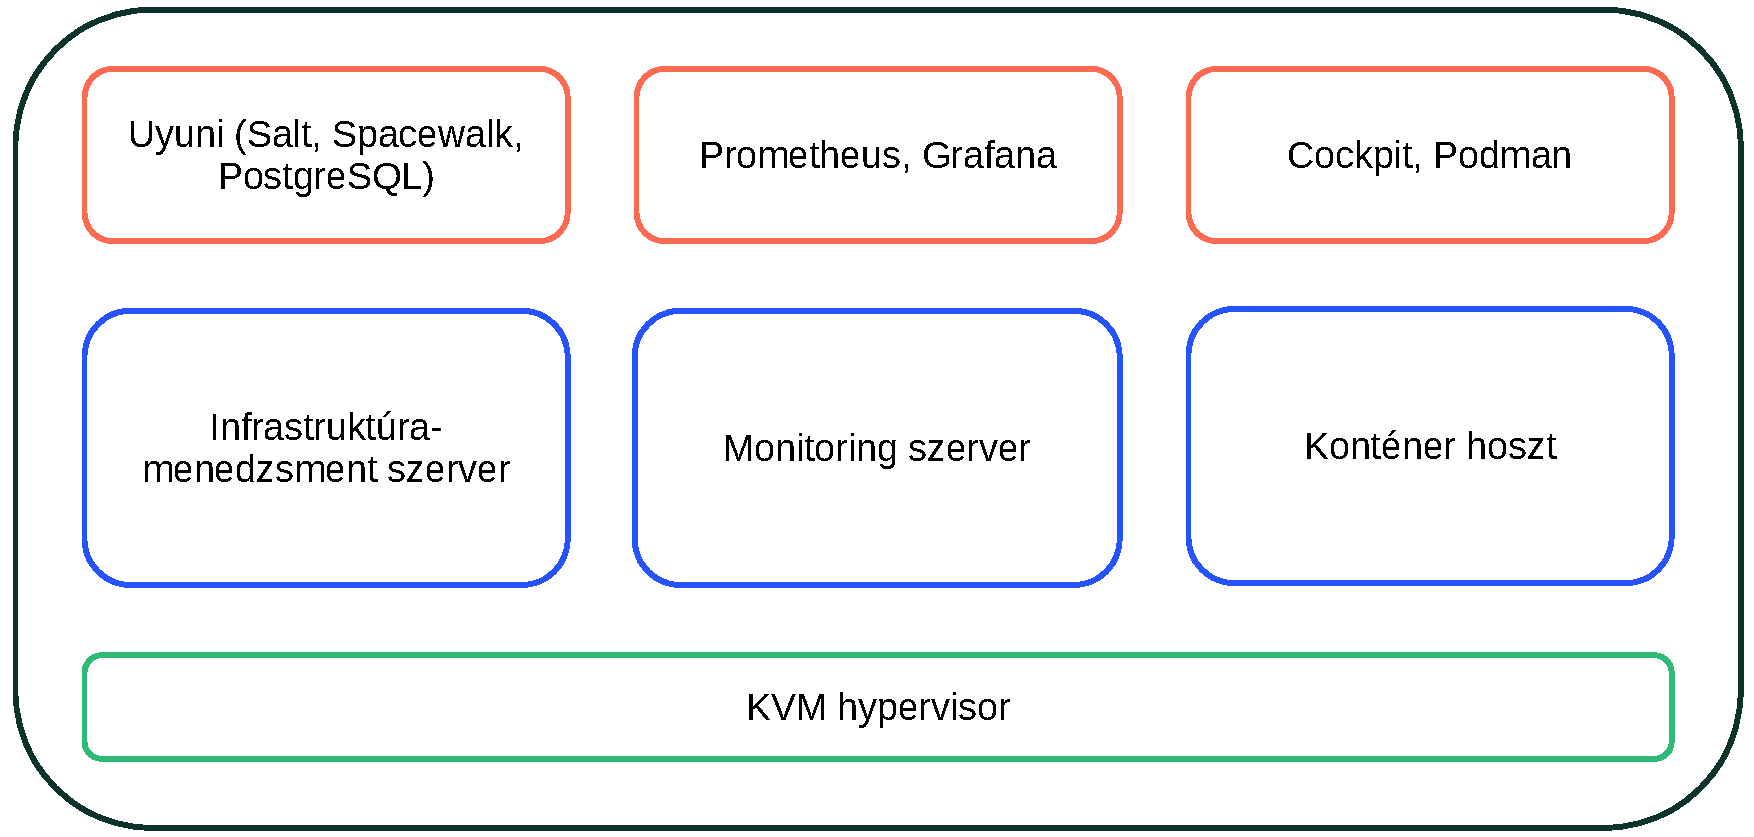
\includegraphics[width=15cm]{figures/architektura.pdf}
	\caption{A tesztkörnyezet tervezett felépítése.}
	\label{fig:test-env-arch}
\end{figure}

\section{Fizikai gép ismertetése}
Ahogy arról \aref{sect:servers} alfejezetben már írtam, a szervergépek több lényeges tulajdonságukban is eltérnek a személyi számítógépektől. A virtualizáció szempontjából legfontosabb ilyen különbségek a processzormagok száma és a memória mennyisége. A tesztkörnyezetet szerettem volna egy ilyen gépen megvalósítani, hogy az ténylegesen a lehető legközelebb állhasson egy valós felhasználási környezethez. Bár a lehetőségeim korlátozottak voltak, sikerült beüzemelnem egy régi, Sun Fire X4450 típusú szervergépet. Ez négy fizikai \acrshort{cpu}-val rendelkezik, mind a négy processzor 6-6 magot tartalmaz, így összesen 24~maggal gazdálkodhattam. Emellett a gép 64~GB memóriával van felszerelve, és egy 1~TB-os \acrshort{ssd}-meghajtó található benne. Ezek mellett a korábban említett hardveres redundancia is megjelenik a gépben: két tápegysége és négy hálózati csatlakozója van, továbbá távolimenedzsment-porttal is rendelkezik, mely lehetővé teszi a szerver távolról történő ki- és bekapcsolását, illetve a rendszernaplók böngészését.

\begin{figure}[!ht]
	\centering
	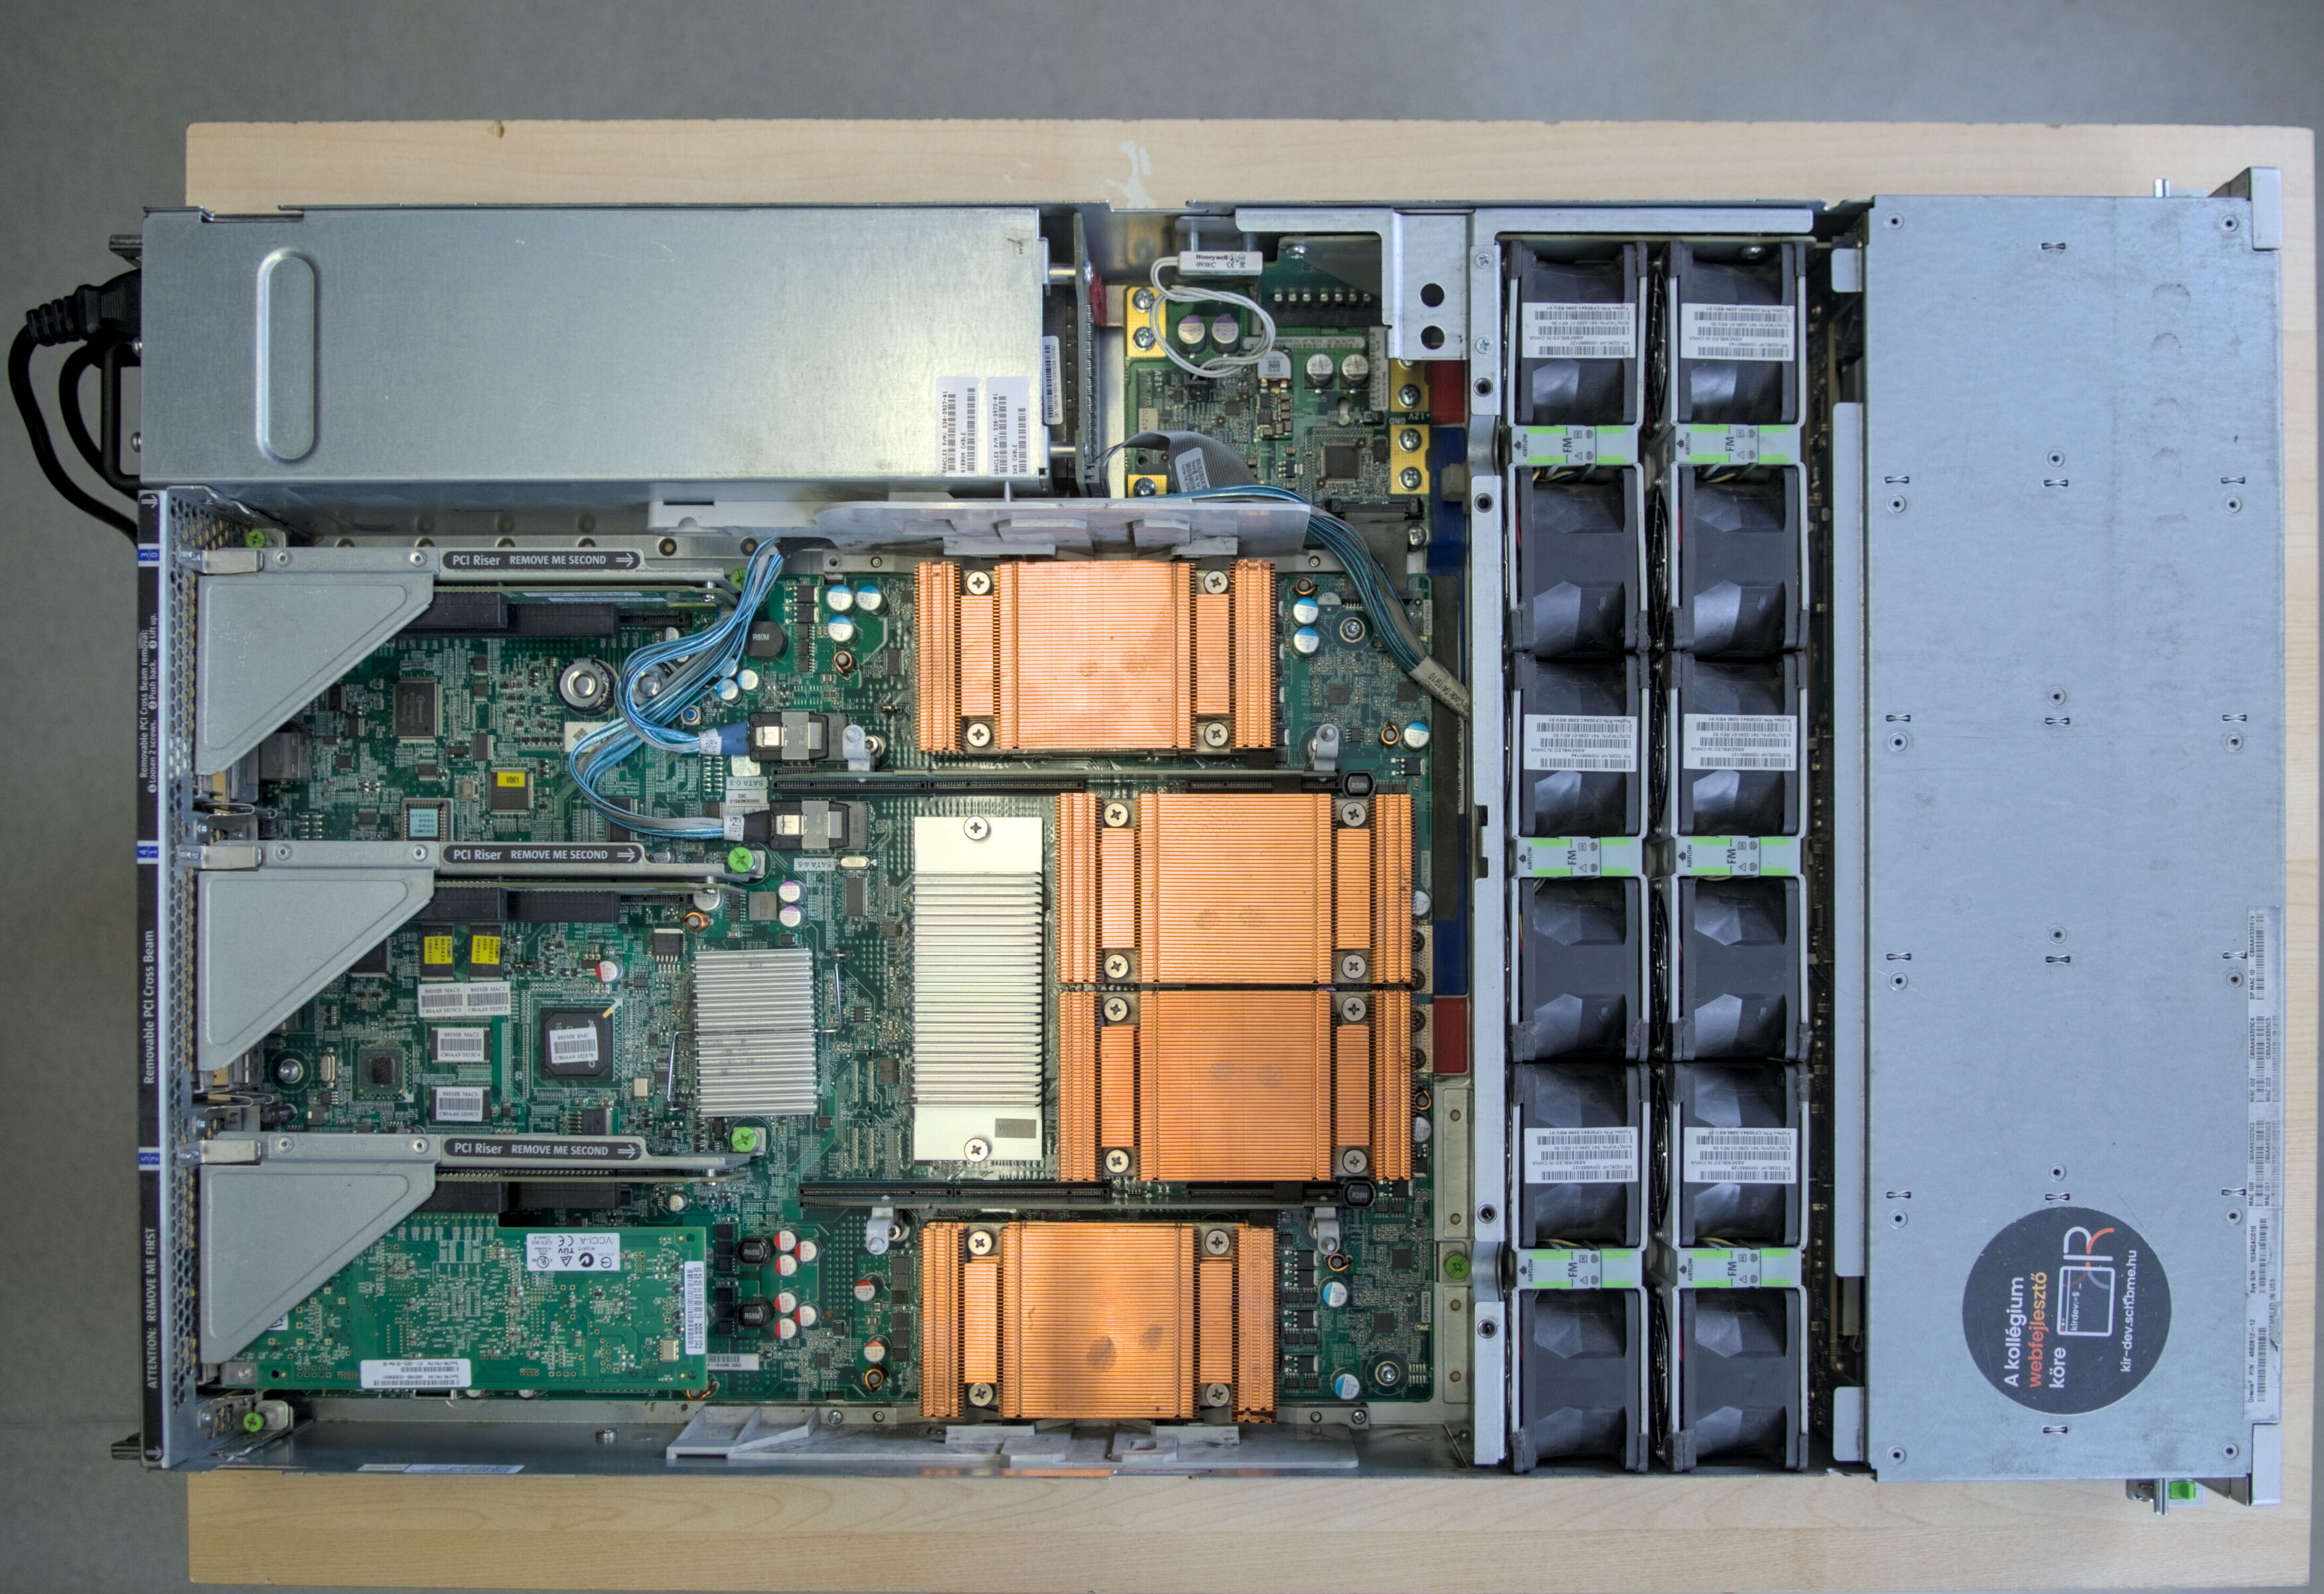
\includegraphics[width=15cm]{figures/szerver.jpg}
	\caption{A tesztkörnyezetben használt fizikai gép. A fotón megfigyelhető a moduláris felépítés, a memóriatálcát eltávolítva pedig a négy különálló \acrshort{cpu} is láthatóvá válik.}
	\label{fig:server}
\end{figure}

\section{Operációs rendszer}
Értekezésemben nagy szerepe lesz a választott operációs rendszereknek, hiszen ezek fognak a virtualizációs rendszer alapjául szolgálni, valamint képesnek kell lennünk a gépek távoli menedzsmentjére is, így mindenképpen olyan megoldásra van szükség, amely jól támogatott a választott infrastruktúramenedzsment-eszköz által. Fontos szempont volt továbbá, hogy a tesztkörnyezet a lehetőségekhez mérten jól képviselje a nagyvállalati környezetben használatos rendszereket, így sok olyan OS-verzió kikerült a lehetőségek közül, amelyek ugyan népszerűek például asztali megoldásként, de egyes nagyvállalati szoftverek (legyen az adatbázismotor, vagy bizonyos eszközvezérlők, driverek) hivatalosan nem támogatottak rajtuk. Emiatt az operációs rendszerek kiválasztása során körültekintően jártam el, több Linux-disztribúció is szóba került, az ezekről született konklúziót itt foglalom össze néhány mondatban.

\subsection{OS-kiválasztás folyamata}
Ahogy \aref{sect:os}. alfejezetben is kitértem rá, a nagyvállalatok elsősorban a Red Hat és a SUSE Linux-disztribúciók közül választanak, hiszen ezeknek a velük együtt járó támogatás és a szoftvercsomagok széleskörű támogatottsága miatt kényelmesebb és hatékonyabb az üzemeltetésük, valamint biztonsági szempontból is kedvezőbbek (például gyorsabban kapnak meg bizonyos frissítéseket, patcheket). Szintén jobban támogatottak ezeken a rendszereken a különböző felhasználásspecifikus modulok, például \acrfull{ha}, live patching (támogatás pl. kritikus kernel biztonsági javítások telepítése a számítógép újraindítása nélkül) és real time computing (valós idejű, nagy időbeli pontosságot igénylő alkalmazások futtatására alkalmas környezet).

A fent ismertetett szélesebb körű támogatottság miatt a tesztkörnyezethez használni kívánt operációs rendszerek köre a Red Hat-re és a SUSE Linuxra korlátozódott. A végső döntésben végül az alábbi szempontok segítettek:
\begin{itemize}
	\item a tesztkörnyezetet szerettem volna egy ökoszisztémán belül tudni mind a virtuális gépeket futtató, mind pedig az azokon futó \acrshort{os}-ek esetében,
	\item könnyebb konfigurálhatóság: mivel több gépet kellett telepíteni, így fontos szerepe volt annak, hogy egy-egy operációs rendszer telepítése milyen bonyolultságú,
	\item a környezetet a költségek minimalizálása mellett szerettem volna létrehozni, így lényeges szempont volt, hogy az adott rendszerhez ne kelljen előfizetést vásárolni, mégis a lehető legközelebb álljon a kereskedelmi forgalomban kapható termékekhez.
\end{itemize}

Mindezek figyelembevételével és korábbi tapasztalataim alapján a SUSE termékcsaládja mellett döntöttem. A támogatással rendelkező, előfizetéses modellt használó nagyvállalati változat mellett szabadon beszerezhető openSUSE operációsrendszer-család megfelelt a tesztkörnyezettel szemben támasztott elvárásaimnak. A rendszer telepítését és a későbbi konfigurációt a YaST keretrendszer segíti, mely számos moduljával (pl. particionálás, hálózati és tűzfalbeállítások) nagyban hozzájárul a gépek könnyebb beállításához, kezeléséhez. A YaST -- mivel szervereken való használatra tervezték, melyek gyakran nem rendelkeznek grafikus felülettel -- \aref{fig:yast-partitioner} ábrán látható megjelenés mellet egy konzolos, GUI-szerű (GUI-like) felülettel is rendelkezik, így a konfiguráció kényelmesen elvégezhető konzolos hozzáférés, például \acrshort{ssh} használata esetén is.

% TODO: yast kép olvashatóság ellenőrzése
\begin{figure}[!ht]
	\centering
	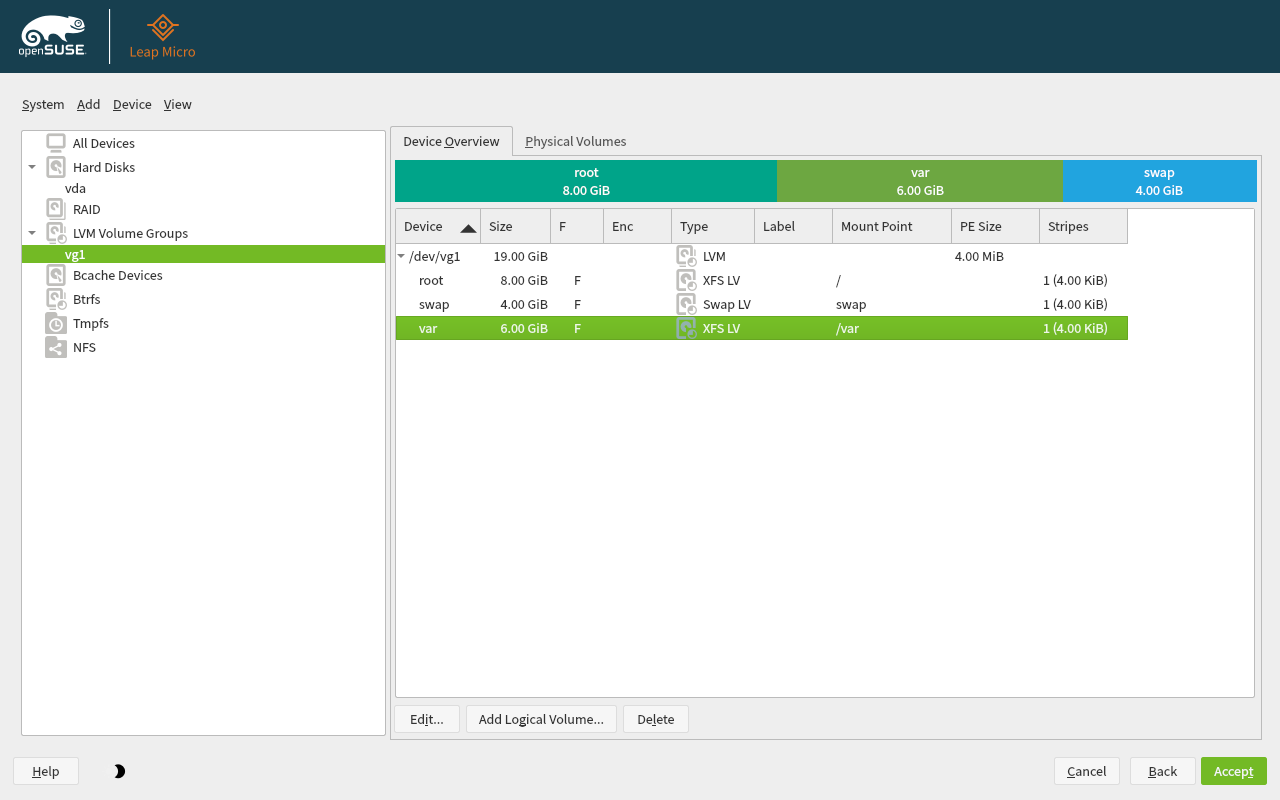
\includegraphics[width=15cm]{figures/yast-partitioner.png}
	\caption{\acrshort{lvm}-kötetek létrehozása openSUSE Leap Micro telepítése során grafikus YaST telepítő segítségével.}
	\label{fig:yast-partitioner}
\end{figure}

Az openSUSE-projekt több operációs rendszert is fejleszt\footnote{\url{https://get.opensuse.org/}}, ezek közül én a tesztkörnyezetben kettőt használtam, melyeket a következő alfejezetekben ismertetek.

\subsubsection{openSUSE Leap}
A Leap egy hagyományos értelemben vett szerver operációs rendszer. Gyakran kap biztonsági frissítéseket, új verziói pedig körülbelül évente jelennek meg. Alapjául a \acrfull{sle} szolgál, melynek előnye, hogy a két rendszer csomagjai binárisan kompatibilisek egymással, azaz egy \acrshort{sle}-rendszerre készített csomag garantáltan használható openSUSE Leap-en is, és fordítva~\cite{openSUSELeap15SP3intro}~\cite{SLE15SP3intro}. Utóbbi előnye, hogy így számos, a közösség (akár a hivatalos openSUSE projekt, akár a felhasználók) által készített csomagot használhatunk a \acrshort{sle}-alapú rendszerünkön is, bár ehhez nem kapunk hivatalos támogatást.

A nagyvállalati rendszerből való leszármazás másik nagy előnye, ami fontos volt számomra a kiválasztási folyamat során, hogy így gyakorlatilag a \acrlong{sle} egy ingyenes verzióját használhatom, mely lényegében teljesen megegyezik a vállalati környezetben használt megoldással, és előfizetés nélkül is kap frissítéseket, így folyamatosan naprakészen tartható. A biztonsági javításokat illetően fontos megjegyezni, hogy a Leap rendelkezik egy olyan csomagforrással (repository) is, mely a \acrlong{sle}-ban is elérhető frissítéseket tartalmazza, így az ott hozzáférhető fontos javításokat is telepíthetjük a Leap-et futtató rendszereinkre~\cite{openSUSELeapSLERepo}.

\subsubsection{openSUSE MicroOS}
A MicroOS egy újfajta megközelítést használó, modern operációs rendszer, mely elsősorban konténerizált alkalmazások futtatásához készült. \Az{\acrshort{os}} előnye, hogy az alap telepítés csak egy minimális szoftvercsomagot tartalmaz, így az erőforrásigénye elenyésző. A MicroOS egy írásvédett (read-only) BTRFS fájlrendszerű gyökérkönyvtárral rendelkezik, melynek előnye, hogy magas szintű támogatást nyújt fájlrendszer-pillanatképek (filesystem snapshots) kezelésére.
Erre a technológiára épít a MicroOS filozófiája: atomi frissítéseket támogat, ami azt jelenti, hogy egy csomag vagy frissítés telepítése során nem az éppen használatban lévő partíció változik, hanem egy új snapshotba kerülnek a módosítások, mely -- amennyiben a módosítás sikeresen lezajlott -- a következő bootolási folyamat során aktívvá válik, és \az{\acrshort{os}} erről kerül betöltésre, így ekkor már használhatjuk a telepített csomagokat. Az atomi frissítések lényege, hogy a módosítások csak akkor lépjenek életbe, ha a teljes folyamat hiba nélkül futott le, azaz például ha egy művelet során a módosítandó 100 csomagból akár csak egy nem tud települni valamilyen hibából eredendően, akkor a teljes telepítés meghiúsul, ezzel elkerülve azt, hogy a rendszer inkonzisztens állapotba kerüljön. A MicroOS ezáltal képes biztosítani azt, hogy a rendszerünk mindig használható állapotban legyen.

A snapshotok fontos tulajdonsága, hogy mindaddig, amíg nem kerülnek törlésre, használatukkal a rendszer bitről bitre visszaállítható abba az állapotba, amiben a pillanatkép készítésekor volt. Ennek nagy jelentősége lehet egy félresikerült rendszerfrissítést követően, hiszen a korábbi állapotra visszaállva a rendszer zavartalanul folytathatja a működést a hiba elhárításáig.
A probléma okának felderítését segíti a snapshotok felcsatolásának lehetősége: ez azt jelenti, hogy a BTRFS fájlrendszer képes arra, hogy a éppen használt partíció mellett az ahhoz tartozó pillanatképeket is felcsatoljuk, sőt, a két állapotot össze is vethetjük a verziókezelő rendszerekben megszokott módon (erre például a YaST beépített támogatással rendelkezik), mely tovább könnyítheti a hiba forrásának felderítését.
% TODO: btrfs diff ábra

A MicroOS különlegességei közé tartozik még, hogy a szerver operációs rendszereknél megszokott konzolos és távoli asztalos elérés mellett egy webes felületet is biztosít a rendszer kezelésére. Ehhez a Cockpit adminisztrációs rendszert használja, mely az utóbbi években egyre nagyobb népszerűségnek örvendő megoldás. A Red Hat disztribúciói például már ezt a rendszert ajánlják a virtualizáció kezelésére a korábban megszokott virt-manager helyett~\cite{RHELDeprecated}.

A Cockpit felülete gyors áttekintést nyújt a rendszer állapotáról, továbbá könnyíti a konténerek létrehozását (\ref{fig:cockpit-container}.~ábra) és kezelését. A fontosabb metrikák (processzor-, memória-, háttértár és hálózathasználat) megtekintése mellett szükség esetén közvetlenül is be tudunk avatkozni a rendszer működésébe, ugyanis a felület egy terminállal is rendelkezik. Továbbá a futó szolgáltatások állapotát is figyelemmel kísérhetjük, valamint a felhasználói fiókokat is kezelhetjük a Cockpit segítségével.

\begin{figure}[ht]
	\centering
	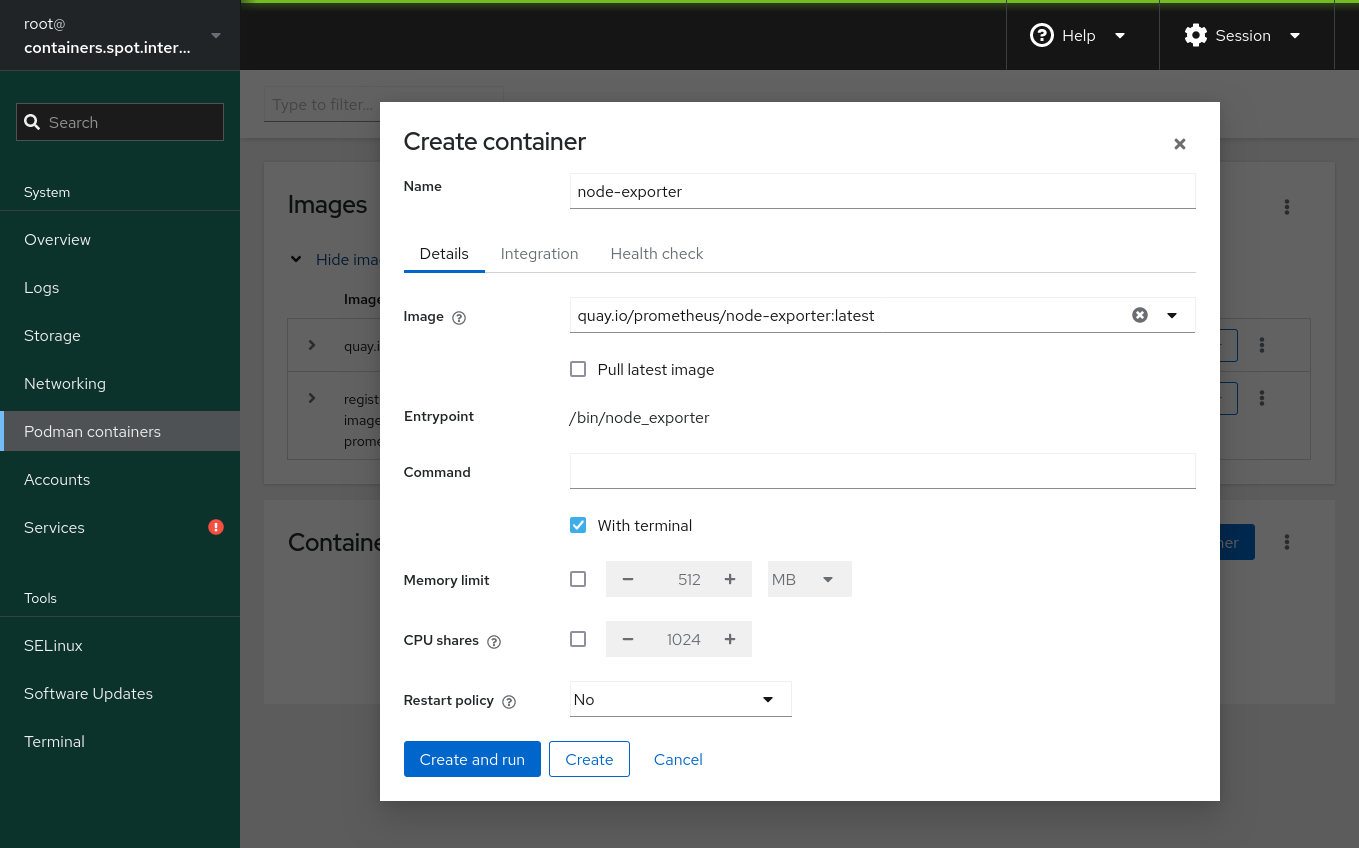
\includegraphics[width=15cm]{figures/cockpit.png}
	\caption{Konténer létrehozása openSUSE Leap Micro-n, a Cockpit webes felületén keresztül.}
	\label{fig:cockpit-container}
\end{figure}

Az openSUSE-projekt kétféle MicroOS-verziót tart karban: a MicroOS-t, mely egy rolling release modellt követ, azaz a rendszer folyamatosan (akár napi szinten) kapja meg a frissítéseket, így több, kisebb verzióugrással tartható karban, míg az openSUSE Leap Micro a \acrlong{sle} Micro kiadási modelljét követi, és a Leap-hez hasonlóan bináris kompatibilitást garantál a két verzió között. A tesztkörnyezethez a stabilitás és kompatibilitás miatt a Leap Micro változatot választottam.

\section{Hálózati topológia}
Az infrastruktúra működésében fontos szerepe van a hálózatnak: a távoli elérésen túl biztosítani kell a szoftvercsomagok elérhetőségét is, valamint a későbbiekben látni fogjuk, hogy a monitoring rendszer is hálózaton keresztül gyűjti az adatokat. Ezek miatt lényeges volt, hogy a gépek tudjanak kommunikálni egymással és a külvilággal. A tesztkörnyezet hálózati felépítését \aref{fig:test-env-network}.~ábra szemlélteti.

\begin{figure}[ht]
	\centering
	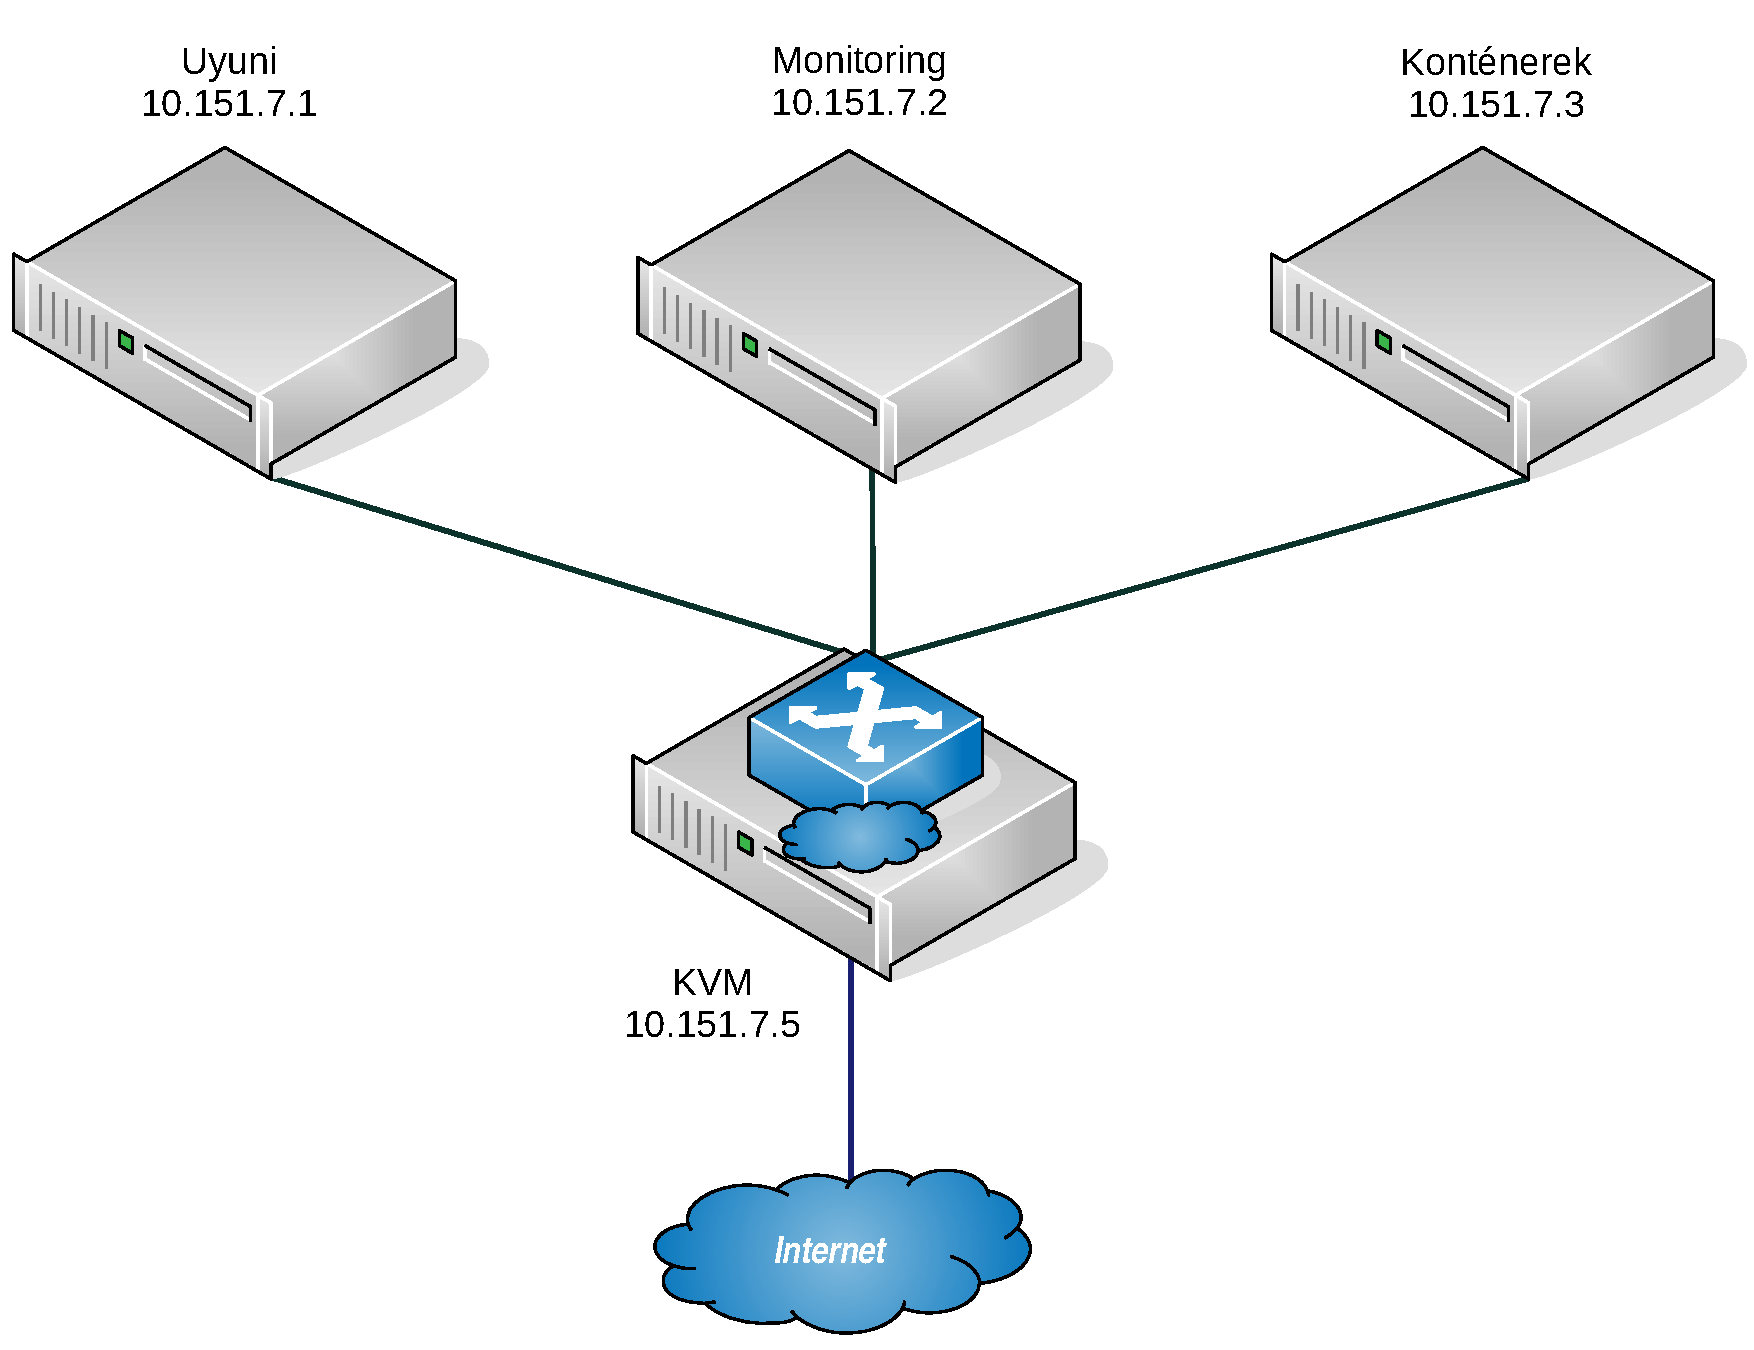
\includegraphics[width=15cm]{figures/halozat.pdf}
	\caption{A tesztkörnyezet hálózati felépítése. Az ábrán nem szerepel a szervergép \texttt{10.151.7.4}-es IP-című menedzsment portja.}
	\label{fig:test-env-network}
\end{figure}

\subsection{Bridge-dzselt hálózati interfész}
\label{sect:net-bridge}
A virtualizált környezetek sajátossága, hogy a virtuális gépek alapesetben egy -- a virtualizációt biztosító szoftver által kezelt -- hálózatra tudnak csatlakozni, a fizikai gép hálózatán nincs lehetőségük kommunikálni. Ez a megoldás általában külön konfiguráció nélkül elérhető, viszont hátránya, hogy a külvilág felé gyakorlatilag láthatatlanná válik a virtuális gép. Bár ez porttovábbítással és a tűzfalbeállítások, valamint az érintett szolgáltatások módosításával orvosolható, a hálózati interfészek bridge-dzselése egy szélesebb körben használható megoldást nyújt.

Egy bridge-dzselt interfész lehetővé teszi a virtuális gépek számára, hogy a gazdagéppel azonos hálózaton kommunikáljanak, azaz ugyanúgy működjenek, mintha minden virtuális gép virtualizált hálózati interfészéhez tartozna egy dedikált hálózati csatlakozó a fizikai gépen, mely egyazon hálózathoz csatlakozik. Ehhez a gazdagép hálózati beállításaiban létre kell hozni egy hálózati híd eszközt, és a használni kívánt interfészt be kell állítani bridge masterként.
Ezeket a beállításokat egyszerűen elvégezhetjük parancssori felületen, illetve a YaST segítségével is (\ref{fig:yast-net-bridge}.~ábra). Az így létrejött virtuális eszköz az OSI-modell szerinti második szinten, az adatkapcsolati rétegben működik a hardveres switch-ekhez hasonlóan~\cite{SUSENetBridge}.

\begin{figure}[ht]
	\centering
	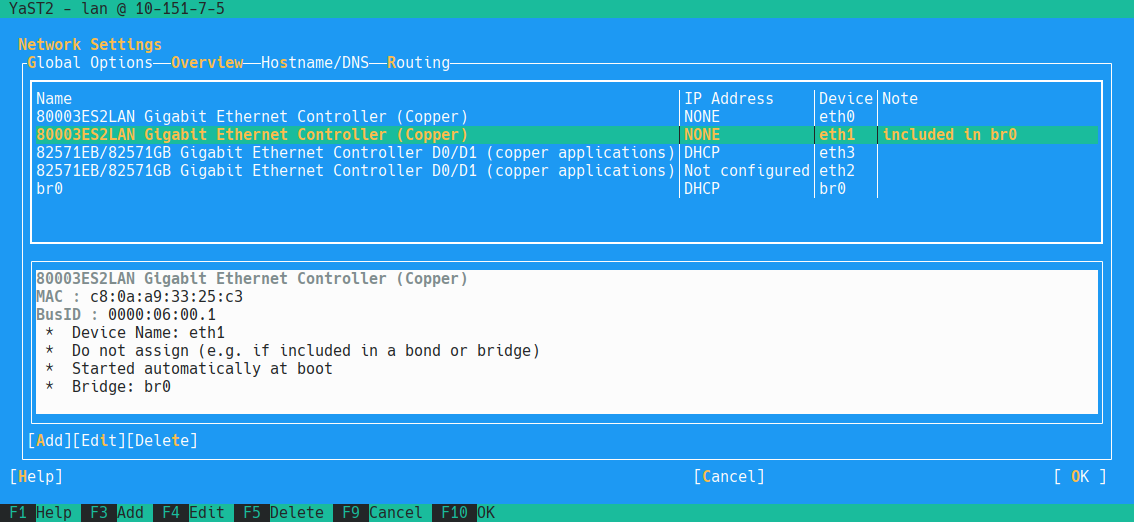
\includegraphics[width=15cm]{figures/yast-br0.png}
	\caption{A tesztkörnyezethez beállított hálózati bridge alapjául szolgáló eth1 fizikai~interfész beállításainak részletei a YaST konfigurációs program parancssori változatában. Látható, hogy az eth1~interfész a br0~bridge eszközhöz van társítva, és előbbihez emiatt nincs hozzárendelve IP-cím.}
	\label{fig:yast-net-bridge}
\end{figure}

\section{Virtualizációs komponensek telepítése}
A tesztkörnyezet szoftveres alapját a virtualizációs megoldások adják. Ebben az alfejezetben ismertetem a fizikai gép előkészítését és a virtuális gépek telepítésének folyamatát, valamint az ezekhez kapcsolódó beállítási lépéseket, kitérve például a particionálás folyamatára és a virtuális gépek terminálos elérésére.

\subsection{Hosztgép konfigurálása}
A virtualizációs környezetet futtató számítógépre az openSUSE Leap 15.5-ös verzióját telepítettem, mely a tesztkörnyezet kialakításakor a disztribúció legfrissebb stabil elérhető változata. A telepítés során a gép szerepének (system role) a szerver opciót választottam. Ez a felhasználási céloknak teljesen megfelelt, hiszen ez a megoldás is egy jól felszerelt operációs rendszert telepít, csak asztali környezet nélkül. Mivel a szervert elsősorban konzolos felületen, \acrshort{ssh}-n keresztül szerettem volna használni, ezért ez nem jelentett gondot. Sőt, a tesztkörnyezet szempontjából előnnyel is járt: a rendszerre nem volt szükséges az asztali környezet működéséhez elengedhetetlen csomagok telepítése, ami nem csak a tárhellyel való takarékoskodásban segített, de a későbbiekben is könnyítette a karbantartási folyamatokat, mert kevesebb csomagot kellett frissíteni és így az esetleges támadási felület (sérülékenységek száma) is kisebb volt. Lényeges azonban megjegyezni, hogy az X11 könyvtár a szerver csomag részeként is telepítésre került, így adott volt a lehetőség X~forwarding\footnote{Távoli szerveren futtatott, grafikus felülettel rendelkező alkalmazások ablakának a kliensgép képernyőjén való megjelenítését lehetővé tevő technológia.} használatára.

A hálózatkezeléshez -- a virtuális gépek hálózati elérését lehetővé teendő -- \aref{sect:net-bridge}.~alfejezetben bemutatott bridge-dzselt hálózati interfészt állítottam be. Ehhez az alapértelmezett beállításokhoz képest annyit kellett módosítani, hogy a bridge-dzselt eszköz a fizikai interfészen keresztül kommunikáljon, illetve hogy a virtualizációs hosztnak kiosztott \texttt{10.151.7.5}-ös IP-címet ne az \texttt{eth1} fizikai interfész kapja meg, hanem az újonnan létrehozott \texttt{br0} eszköz. Ezt követően a számítógép a korábban megszokott módon tudott a hálózaton kommunikálni, viszont lehetővé vált, hogy a virtuális gépek is hozzáférjenek a fizikai gép hálózatához a bridge eszközön keresztül.

A hálózaton kívül a másik lényeges tervezői döntés a logikai kötetek (\acrshort{lvm}) alkalmazása volt. Ez a gyakorlatban azt jelentette, hogy a boot partíció kivételével minden egyéb kötetet \acrshort{lvm}-kötetként hoztam létre. Ennek legfőbb előnye számomra a kötetek méretének rugalmas kezelése volt, melyről \aref{sect:lvm}. alfejezetben írtam bővebben. Emellett lehetőséget biztosít pillanatképek készítésére is, melyek készítése például \acrshort{os}-frissítések előtt lehet releváns, és nagyban megkönnyíti rendszer korábbi állapotának helyreállítást, ha valami hiba jelentkezik a folyamat során. A kötetkiosztás úgy történt, hogy minden virtuális gép kapott egy külön \acrshort{lvm}-kötetet, amit egy egyedülálló tárolóeszközként érzékelt, és ezt használhatta az adatok tárolására, akár további particionálás mellett is.

A kezdetleges konfigurációt követően telepítettem a \acrshort{kvm} \gls{hypervisor}t és a virtuális gépek kezeléséhez szükséges csomagokat. Ehhez openSUSE-disztribúciókon külön ún.~pattern áll a rendelkezésünkre. Ez azt jelenti, hogy nem kell megadnunk minden telepítendő csomagot, hanem elég a \texttt{kvm\_server} és a \texttt{kvm\_tools} pattern-ök telepítése, és ezek automatikusan telepítésre jelölik a teljes értékű \acrshort{kvm}-szerverhez szükséges csomagokat, emellett néhány hasznos segédprogramot (pl. virt-manager, virsh) is magukkal hoznak. Ezen csomagok telepítését követően minden előfeltétel adottá vált a virtuális gépek telepítéséhez.


\subsection{Virtuális gépek telepítése}
\acrshort{vm}-ek telepítéséhez elsősorban a \texttt{virt-install} parancsot használtam. Ez a program lehetővé teszi az összes lényeges paraméter megadását, majd távoliasztal-protokoll használatával (alapértelmezetten \acrshort{spice}, de választhatjuk például a \acrshort{vnc}-t is) megjeleníti a virtuális gép kijelzőjét egy ablakban, melynek segítségével személyre szabhatjuk a telepítést és telepíthetjük az operációs rendszert. A távoli asztalon keresztüli elérés csak a megfelelő környezet, pl. \acrshort{ssh} használata esetén, X~forwardinggal működik. Amennyiben a virt-install nem talál kijelzőt, akkor a telepítés parancssoron keresztül történik. A virt-install sikeres futás esetén egy virtuálisgép-leíró XML-fájlt hoz létre, mely a gép összes paraméterét tárolja~(\ref{lst:virshxml}.~kódrészlet). A későbbiekben a \acrshort{vm} konfigurációjának módosítása esetén ezt a fájlt kell módosítanunk (akár szövegszerkesztővel, akár GUI-n, például virt-manager-rel). A leírófájl a virtuális gép migrációjához is használható.

Azonban még mielőtt a konkrét telepítést elkezdhetnénk, létre kell hoznunk azt a partíciót, melyre a virtuális gép adatai kerülnek. Esetemben ez azt jelentette, hogy az egyes virtuális gépekhez új \acrshort{lvm}-köteteket kellett létrehoznom. Mivel a logikai kötetek számára otthont adó partíciót és a kapcsolódó fizikai kötetet és kötetcsoportot már a hoszt~\acrshort{os} telepítésekor létrehoztam, ezért a~\acrshort{vm}-ek telepítése során elég volt csak egy-egy logikai kötetet~(\acrshort{lv}) létrehoznom, melyhez az \texttt{lvcreate} parancsot használtam~(\ref{lst:lvcreate}~kódrészlet).
Emellett telepítési forrást is meg kellett adni, melyhez én telepítő lemezképeket használtam. Ilyenkor a~\acrshort{vm} telepítésekor fel kell venni egy virtuális CD-meghajtót a géphez, és meg kell adni a telepítési forrás elérési útját.

\begin{lstlisting}[caption=Virtuális gépek logikai kötetének létrehozásához használt parancs.,label=lst:lvcreate]
	lvcreate -L 20G --name kvm-monitoring vg1
\end{lstlisting}

Ezen túl meg kell adni a gép fontosabb paramétereit is (pl. processzorok száma, memória mennyisége), hogy milyen erőforrásokkal szeretnénk telepíteni azt. A tesztkörnyezetben használt gépek telepítése során elsősorban a dokumentációban ismertetett rendszerkövetelményeket vettem figyelembe az erőforrások meghatározásánál, de mivel aránylag sok erőforrás állt rendelkezésemre, így előfordult, hogy a számítási műveletek gyorsítása érdekében a szükségesnél több magot adtam a virtuális gépeknek. Mivel a~\acrshort{vm}-ek konfigurációja szabadon változtatható a későbbiekben is (esetleg a gép újraindítása szükséges az érvényre jutásukhoz), ezért ez nem jelentett problémát a későbbiekben sem. Emellett a~\acrshort{kvm} támogatja a memória és processzor erőforrások \gls{overcommit}-olását is, azaz nem jelent problémát, ha esetleg a fizikai gépen elérhetőnél több \acrshort{cpu}-erőforrást osztottunk ki a virtuális gépek számára, bár ennek használatára a dolgozathoz készített tesztkörnyezetben nem volt szükség~\cite{RedHatKvmOvercommit}.
A tesztkörnyezet egyik virtuális gépének telepítéséhez használt parancsot \aref{lst:virtinstall}.~kódrészlet mutatja be.

\begin{lstlisting}[caption=Virtuális gép telepítése a virt-install segédprogrammal.,label=lst:virtinstall]
	virt-install --name uyuni --memory 32768 --vcpus 12 --cdrom /mnt/openSUSE-Leap-15.5-NET-x86_64-Media.iso --os-variant opensuse15.5 --disk /dev/vg1/kvm-uyuni
\end{lstlisting}

\begin{lstlisting}[caption=Virtuális gép leírófájljának részlete.,label=lst:virshxml]
	<memory unit='KiB'>33554432</memory>
	<currentMemory unit='KiB'>33554432</currentMemory>
	<vcpu placement='static'>12</vcpu>
	<resource>
		<partition>/machine</partition>
	</resource>
	<os>
		<type arch='x86_64' machine='pc-q35-7.1'>hvm</type>
	</os>
	...
	<devices>
		<emulator>/usr/bin/qemu-system-x86_64</emulator>
		<disk type='block' device='disk'>
			<driver name='qemu' type='raw' cache='none' io='native' discard='unmap'/>
			<source dev='/dev/vg1/kvm-uyuni' index='1'/>
			<backingStore/>
			<target dev='vda' bus='virtio'/>
			<boot order='2'/>
			<alias name='virtio-disk0'/>
			<address type='pci' domain='0x0000' bus='0x04' slot='0x00' function='0x0'/>
		</disk>
	...
	</devices>
\end{lstlisting}

A virtuális gép operációs rendszerének telepítése során ki kellett alakítani a kívánt partíciókiosztást, mely a felhasználási körtől függően változott, de alapvetően mindenhol \acrshort{lvm}-alapú kötetkiosztást alkalmaztam. Emellett szükséges volt bizonyos hálózati beállítások (pl.~\acrshort{dns}-szerver címe, gépnév) módosítása is. Ezeken felül és az alapvető adatok~--~mint~például felhasználói fiókok létrehozása, lokalizációs beállítások konfigurálása~--~megadásán túl mást nem volt szükséges átállítani a telepítés során. A sikeres installációt követően foghattam hozzá a virtuális gépeken futó szolgáltatások telepítéséhez, melyeket a következő fejezetekben fogok részletesen ismertetni.

% !TeX spellcheck = hu_HU
% !TeX encoding = UTF-8

\chapter{Infrastruktúramenedzsment: Uyuni}
\label{chap:uyuni}
Nagyméretű informatikai infrastruktúra kezelése esetén elengedhetetlen valamiféle infrastruktúramenedzsment-eszköz használata. Ez nem csak könnyebbé teszi az üzemeltetést, de számos kiegészítő funkcióval is rendelkezik, lényegében egy helyen láthatunk minden releváns adatot, és egyazon felületről van lehetőségünk frissítések telepítésére és biztonsági sérülékenységek leírásainak böngészésre, mint ahol azt is tároljuk, hogy egy adott virtuális gép melyik gazdagépen fut, és az hol található.

Mivel ez a megoldás hasznosnak és érdekesnek tűnt számomra, és a dolgozat profiljába is jól illeszkedik, úgy döntöttem, hogy a tesztkörnyezet kezelésére is fogok ilyen megoldást alkalmazni. A választásom az Uyuni-ra esett, mely gyakorlatilag mindent tud, amire szükségem volt, és ingyenesen elérhető. A döntésben az is segített, hogy a projektet a SUSE támogatja, a fejlesztésében is részt vesz (az Uyuni szolgál a kereskedelmi forgalomban lévő SUSE Manager megoldás alapjául), és az openSUSE-alapú disztribúciókra is kiemelt figyelmet fordítanak, így nem kellett kompatibilitási problémákkal foglalkoznom. Az Uyuni a Salt konfigurációmenedzsment és automatizációs keretrendszerre épül, mely szintén széleskörűen használt és támogatott.


\section{Telepítés}
\label{sect:uyuni-install}
Az Uyuni meglehetősen erőforrás-igényes, a telepítéséhez minimum négy CPU-mag, 16~GB memória és  több száz gigabyte tárhely lehet szükséges a használni kívánt telepítőforrásoktól függően~\cite{UyuniInstallGuide}. Éles környezetben még ennél is több memóriát javasolnak, így az Uyuni számára létrehozott virtuális gép lett a környezet leginkább erőforrás-igényes rendszere, melynek telepítéshez használt parancs és a \acrshort{vm} leírója látható \aref{lst:virtinstall} és \aref{lst:virshxml} kódrészleteken. Ezeken megfigyelhetjük, hogy a virtuális gépet 12~CPU-maggal és 32~GB memóriával hoztam létre, a particionálásra a későbbiek folyamán fogok részletesen kitérni.

Ahogy a korábbiakban írtam, az Uyuni jó támogatottságnak örvend az openSUSE platformon. A telepítési kézikönyvben egy dedikált openSUSE Leap 15.5-ös \acrshort{os}-verziót futtató számítógépet javasolnak az infrastruktúramenedzsment-program telepítéséhez~\cite{UyuniInstallGuide}.
Ennek megfelelően én is ezt a verziót telepítettem, és bár a Leap alapértelmezett telepítési forrásaiban nem szerepel az Uyuni, de az ezt tartalmazó telepítőforrást egyetlen paranccsal felvehetjük, és ezt követően a segítségével telepíthetjük is az Uyunit.

\subsection{Kötetkiosztás}
A particionálás kérdése azért is kiemelt fontosságú az Uyuni telepítése során, mert a telepítés folyamán ezen feltételek meglétét ellenőrzi is a telepítő, és nem teljesülésük esetén a telepítés hibára futhat. A kötetek kiosztása során a hivatalos útmutatóból indultam ki, viszont a felhasználási célok figyelembevételével néhány partíciót a javasoltnál nagyobbra állítottam be, ennek megfelelően jött létre \aref{tab:uyuni-partitioning}.~táblázatban ismertetett felépítés. Elsősorban a spacewalk kötet növelése volt indokolt, hiszen az Uyuni egyik fontos része a szoftvercsomagok kezelése. Ennek gördülékeny és hatékony használatához a rendszer letükrözi a szükséges telepítőforrásokat, melyek jelentős helyigénnyel rendelkeznek, melyre \aref{sect:reposync} alfejezetben térek ki részletesen.

\begin{table}[h]
	\setlength{\tabcolsep}{5pt}
	\renewcommand{\arraystretch}{1.3}
	\centering
	\begin{tabular}{||l l l l m{5.3cm}||}
		\hline
		Kötet & Csatolási pont & Méret & Típus & Leírás\\
		\hline\hline
		boot & /boot & 1~GB & fizikai, ext4 & Az \acrshort{os} betöltéséhez szükséges fájlok tárhelye. \\
		\hline
		root & / & 40~GB & \acrshort{lvm}, XFS & A könyvtár-hierarchia legfelső eleme, a rendszerfájlok helye. \\
		\hline
		pgsql & /var/lib/pgsql & 52~GB & \acrshort{lvm}, XFS & A PostgreSQL adatbázismotor által tárolt adatok könyvtára. \\
		\hline
		spacewalk & /var/spacewalk & 100~GB & \acrshort{lvm}, XFS & Az infrastruktúramenedzsment\Hyphdash szoftver által használt fájlok elsődleges helye. \\
		\hline
		cache & /var/cache & 12~GB & \acrshort{lvm}, XFS & Gyorsítótárazott adatok könyvtára. \\
		\hline
		swap & swap & 4~GB & \acrshort{lvm}, swap & Virtuális memóriaként használt lemezterület. \\
		\hline
	\end{tabular}
	\caption{Az infrastruktúramenedzsment-szerver telepítéskori kötetkiosztása.}
	\label{tab:uyuni-partitioning}
\end{table}

\section{Telepítőforrások tükrözése}
\label{sect:reposync}
Ahogy az előző alfejezetben már említettem, az Uyuni egyik központi feladata a telepítőforrások és szoftvercsomagok kezelése a bevont rendszereken. Ehhez a használni kívánt telepítőforrásokat le kell tükröznünk az Uyunit futtató szerverre. Ez a megoldás elsőre túlzásnak tűnhet, hiszen egy-egy ilyen forrás több tíz, egyes esetekben több száz gigabyte lehet, azonban egy nagyméretű infrastruktúránál megvannak az előnyei. Gondoljunk csak bele, hogy mekkora hálózati forgalmat takaríthatunk meg azzal, hogy a telepítendő szoftverek és operációsrendszer-frissítések letöltésekor nem kell minden esetben az internetről letölteni a szükséges csomagokat, hanem ezt elegendő mindössze egyszer, az Uyuni szerveren megtenni, és onnantól kezdve az összes kliens már a belső hálózatról érheti el a szükséges programokat.
Emellett hasznos lehet egy offline példány megtartása is a telepített csomagokból, hiszen előfordulhat, hogy egy harmadik fél által üzemeltetett telepítési forrás elérhetetlenné válik, és így nem férünk hozzá a kívánt csomagokhoz.

Ahhoz, hogy egy-egy ilyen csomagtárhelyet letükrözhessünk, létre kell hozni úgynevezett \textit{Software Channel}-eket, melyek lényegében a repository-t csomagolják be egy magasabb szintű egységbe. Ez tárolja, hogy milyen csomagok érhetőek el, ezek milyen architektúrán használhatóak, lehetővé teszik a csomagforrások kezelését, és hozzárendelhetjük őket a kliensekhez. A csatornák által tartalmazott repository-k tárolják, hogy milyen címen érhető el a tükrözendő telepítőforrás, és hogy az adott repository melyik csatornához van hozzárendelve.

A tesztkörnyezethez is tükröztem telepítési forrásokat. Mivel a gépek többsége openSUSE Leap~15.5-ös verziót használt, ezért az ehhez tartozó csomagok szinkronizálásával kezdtem. Minden alapértelmezett forrást letükröztem, illetve az Uyuni általi menedzselés céljából az Uyuni-csomagokat tartalmazó repository-t is felvettem a szinkronizálandók közé. Az egyszerűbb kezelés miatt a csatornák hierarchiába szervezhetőek, így csak a kiválasztott szülőcsatornával (base channel) kompatibilis gyermekcsatornákat vehetünk fel egy adott klienshez. A tesztkörnyezetben létrehozott telepítőforrás-hierarchiát \aref{fig:software-channels}.~ábra szemlélteti.

\begin{figure}[ht]
	\centering
	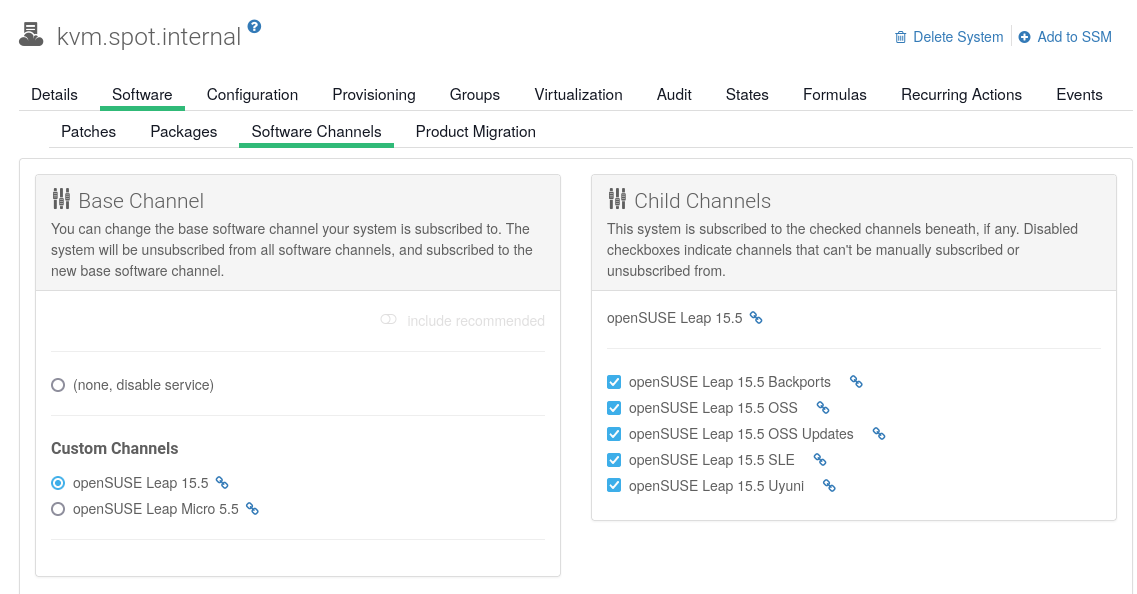
\includegraphics[width=15cm]{figures/uyuni-channels.png}
	\caption{A kialakított csatornahierarchia.}
	\label{fig:software-channels}
\end{figure}

Az első repository tükrözése a vártnál közel 20\%-kal több tárhelyet igényelt a spacewalk köteten (\ref{fig:reposync-disk-usage}.~ábra), így szükségessé vált a partíció megnövelése. Ennek megvalósításához az~\acrshort{lvm} által biztosított \texttt{lvextend} parancsot használtam, mely a logikai kötet megnövelésén túl a fájlrendszer (itt XFS) kiterjesztését is támogatja. Ez a parancs viszont csak akkor használható, ha a kötetcsoportban~(\acrshort{vg}) rendelkezésre áll annyi szabad hely, amennyivel bővíteni szeretnénk a tárhelyet. Mivel azonban itt ez a feltétel nem teljesült, több szinten kellett elvégezni a kötet megnövelését, először a~\acrshort{kvm}-hoszton kellett megnövelni a virtuális géphez tartozó tárterületet. További kihívást jelentett, hogy a kiterjesztést a~\acrshort{vm} leállítása nélkül szerettem volna elvégezni. Ebben az esetben nem jelentett volna nagy gondot a gép újraindítása, viszont szerettem volna felkészülni olyan helyzetekre is, amikor a gép leállítása nem megengedhető. Ilyen lehet például, ha a szinkronizálás alatt álló telepítőforrás a vártnál jelentősen nagyobb méretűnek bizonyul, vagy éppen a~PostgreSQL által használt tárhely van fogytán, de még nem fejeződött be a korábban indított indexelés. Mindezek mellett általában éles környezetben is korlátozottak a lehetőségeink egy-egy kiszolgáló újraindítására.

\begin{figure}[ht]
	\centering
	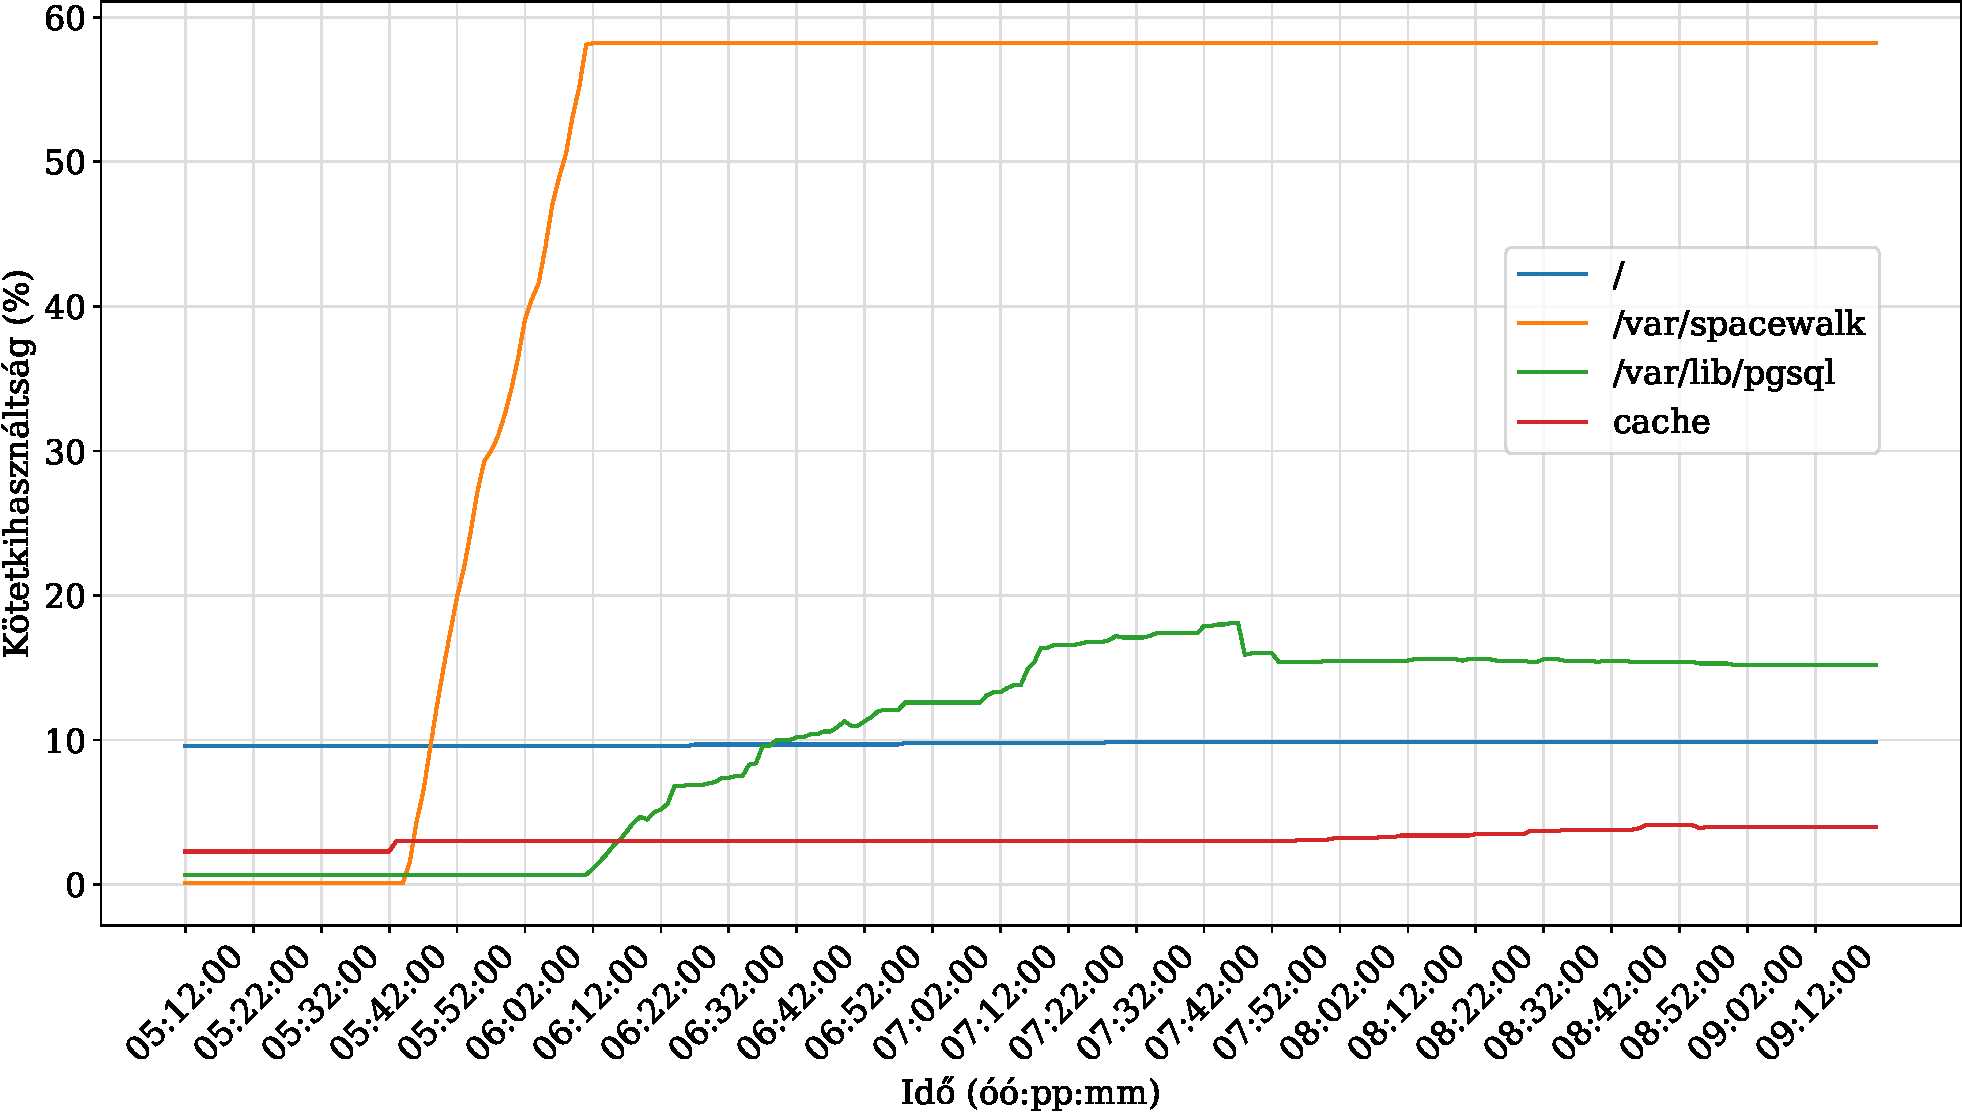
\includegraphics[width=15cm]{figures/reposync-leap-oss-disk-grid.pdf}
	\caption{Kötetkihasználtság változása az egyik telepítőforrás tükrözése során.}
	\label{fig:reposync-disk-usage}
\end{figure}

\subsection{Online kötetnövelés}
Ezen okokból a spacewalk kötet online megnövelése mellett döntöttem. Első lépésként a hosztgépen terjesztettem ki a virtuális gép számára fenntartott partíciót (a~\texttt{kvm-uyuni} logikai kötetet). \Aref{lst:virsh-blockresize}. kódrészleten látható, hogy ezt követően a virtuális gép még nem tudja használni a nagyobb méretű kötetet, szükséges még a \texttt{virsh blockresize} parancs futtatása, melynek hatására a virtuális gép számára is láthatóvá válik a nagyobb kötetméret. Ezt követően a~\acrshort{vm}-en növeltem meg a logikai kötetek alapjául szolgáló fizikai kötet~(\acrshort{pv}) méretét, melyet követően már a megszokott módon volt lehetőség a logikai kötet bővítésére.

\begin{lstlisting}[caption=Az infrastruktúramenedzsment-programokat futtató virtuális gép kötetének online megnövelése a gazdagépen.,label=lst:virsh-blockresize,escapechar=?]
	?\underline{10-151-7-5:$\sim$ \#}? virsh domblkinfo uyuni /dev/vg1/kvm-uyuni
	Capacity:       268435456000
	Allocation:     225145827328
	Physical:       375809638400
	?\underline{10-151-7-5:$\sim$ \#}? virsh blockresize uyuni --path /dev/vg1/kvm-uyuni --size 350G
	Block device '/dev/vg1/kvm-uyuni' is resized
	?\underline{10-151-7-5:$\sim$ \#}? virsh domblkinfo uyuni /dev/vg1/kvm-uyuni
	Capacity:       375809638400
	Allocation:     225145827328
	Physical:       375809638400
\end{lstlisting}

\section{Kliensek felvétele}
A kliensek felvétele során mutatkozott meg az Uyuni egy kisebb hátránya az előfizetés-alapú SUSE~Manager-rel szemben. Míg az előfizetésért cserébe előre konfigurált csatornákat (ún. Product-okat) kapunk, addig az Uyunihoz ez nem áll rendelkezésünkre, a kliensek felvételéhez használt bootstrap megoldás pedig csak ezekkel működik együtt. A bootstrap folyamat sikeres futtatása többszörös próbálkozást követően sem sikerült~(\ref{fig:uyuni-bootstrap-error}. ábra). Emiatt az elsődleges konfiguráció során manuálisan kellett gondoskodnom a szükséges csomagok telepítéséről és az ezekhez kapcsolódó beállítások elvégzéséről. A gyakorlatban ez azt jelentette, hogy a kezelni kívánt rendszerekre telepíteni kellett a \texttt{venv-salt-minion} csomagot, emellett szükséges volt két konfigurációs fájl létrehozása is, melyek a Salt minion azonosítóját (amilyen néven a gép megjelenik az~Uyuni felületén) és a Salt master (az~Uyuni szerver) IP-címét tartalmazták~(\ref{lst:salt-client-config}.~kódrészlet).
Ezt követően a kapcsolódó Salt service újraindításával a kliens kapcsolatot kezdeményezett a Salt masterrel, és az Uyuni felületén lehetővé vált a kliens csatlakozási kérelmének elfogadása. A kérelem elfogadását követően az Uyuni lekérdezett néhány adatot a kliens állapotáról (pl. telepített csomagok, hardveres erőforrások), ez után az újonnan bevont rendszer már teljes körűen kezelhetővé vált az Uyuni felületén keresztül.

\begin{figure}[ht]
	\centering
	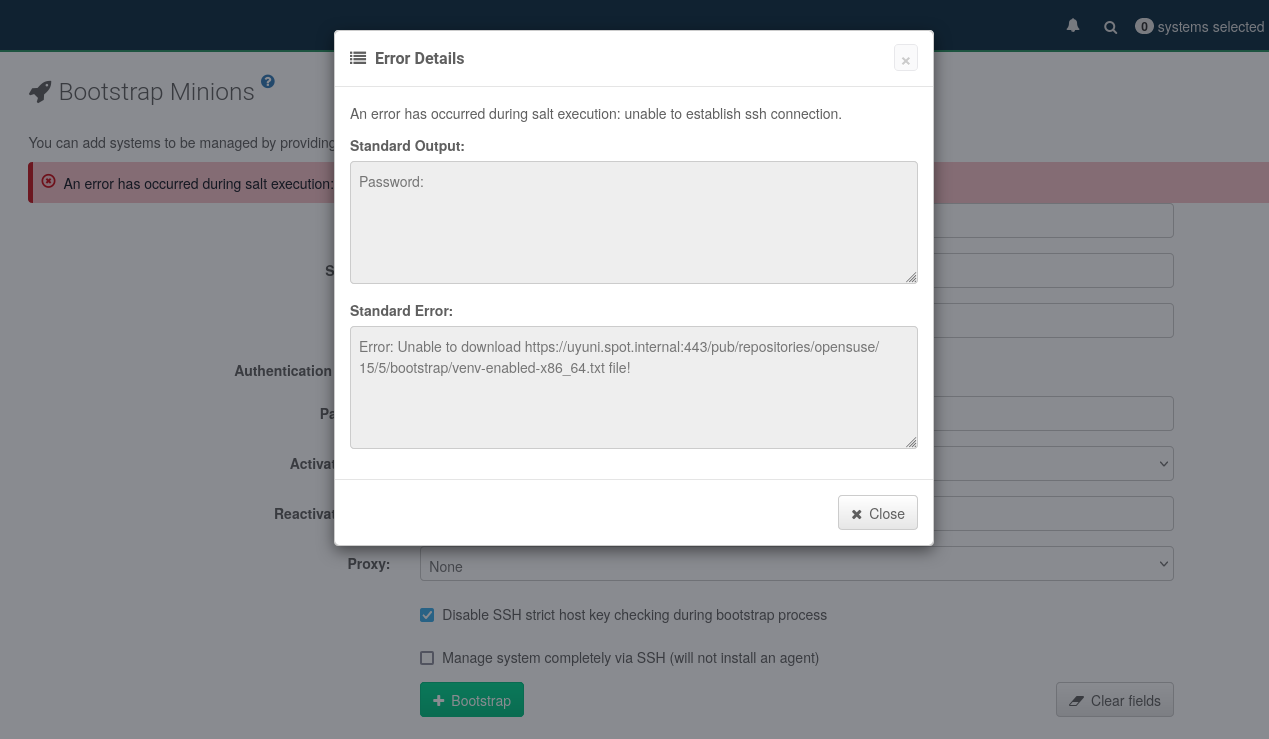
\includegraphics[width=15cm]{figures/uyuni-bootstrap-error.png}
	\caption{Előfizetés nélkül nem érhetőek el a product repository-k.}
	\label{fig:uyuni-bootstrap-error}
\end{figure}


\begin{figure}[ht]
	\centering
	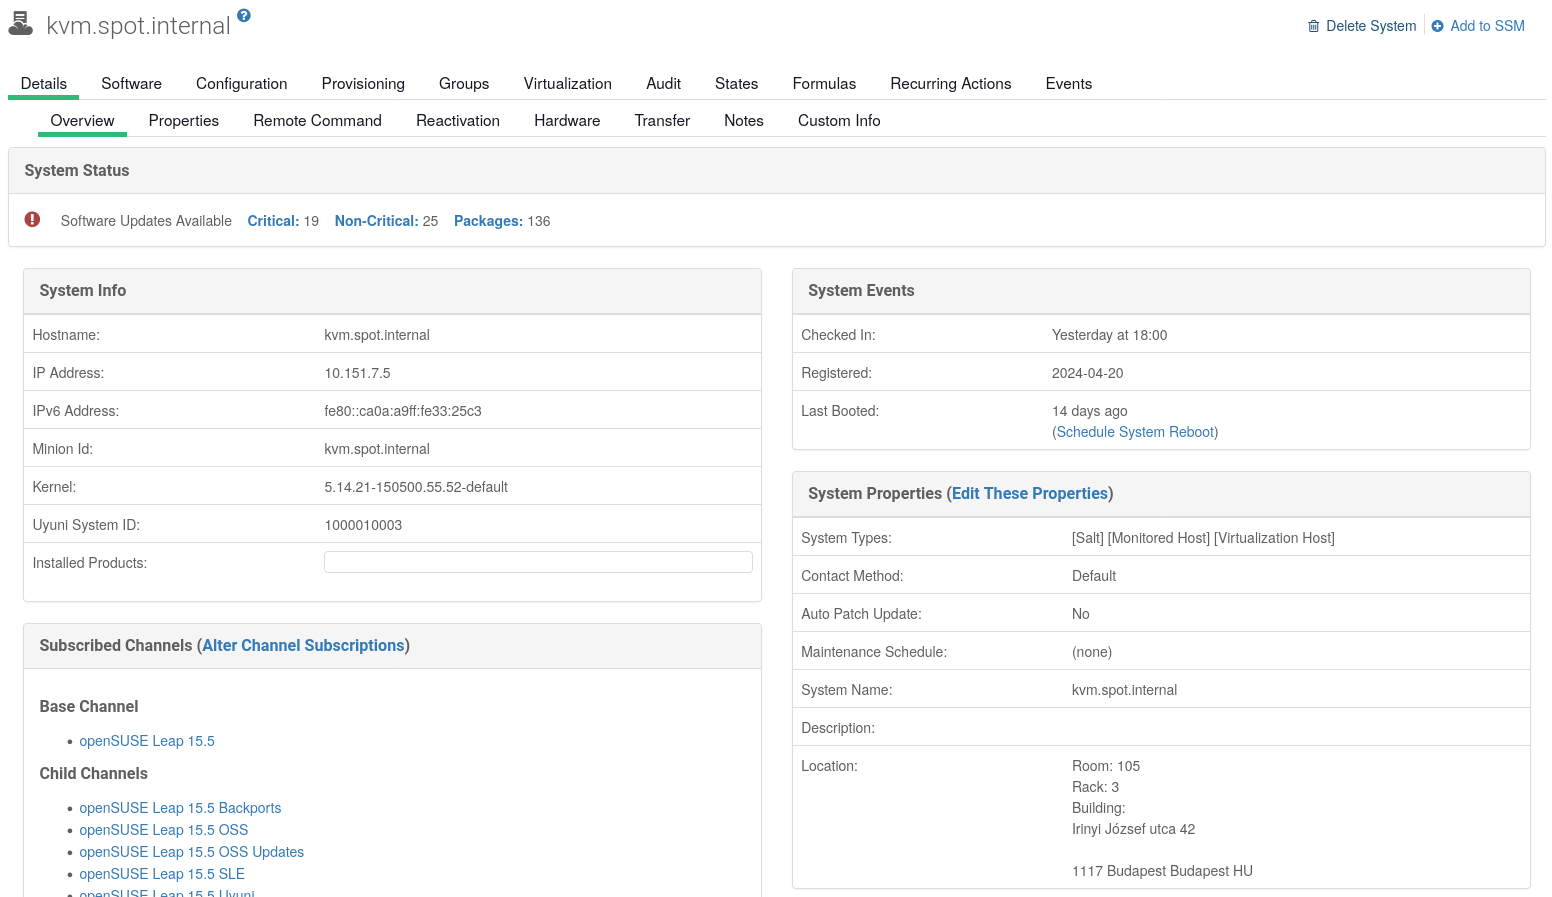
\includegraphics[width=15cm]{figures/uyuni-system-details.png}
	\caption{A bevont rendszer adatainak frissítését követően számos részletet láthatunk a gépről, és mi is adhatunk meg bizonyos adatokat.}
	\label{fig:uyuni-system-details}
\end{figure}

\begin{lstlisting}[caption=A manuális konfiguráció során létrehozott állományok.,label=lst:salt-client-config,escapechar=?]
	?\underline{10-151-7-5:/etc/venv-salt-minion/minion.d \#}? cat id.conf
	id: kvm.spot.internal
	?\underline{10-151-7-5:/etc/venv-salt-minion/minion.d \#}? cat master.conf
	master: 10.151.7.1
\end{lstlisting}

\subsection{Rendszertípusok és Salt Formulák}
A kezdeti információgyűjtés során az infrastruktúramenedzsment-rendszer megpróbálja meghatározni a rendszer típusát (fizikai gép, virtualizációs gazdagép, virtuális gép). Ezeket később mi is megadhatjuk, illetve a betöltött szereptől függően úgynevezett Salt Formulákat rendelhetünk hozzájuk. Ezek olyan előre elkészített Salt state fájlok, melyek a gyakran használt beállítások megadását igyekszenek egyszerűbbé tenni.

Munkám során én két rendszertípust használtam: a virtualizációs hoszthoz és a monitorozott rendszerhez kapcsolódót. A \textit{Virtualization Host} Formula néhány alapvető beállítást (pl. hálózati konfiguráció) ad meg a rendszeren, azonban ez a felhasználási céljaimnak nem felelt meg teljes mértékben, így a beállításokat egy saját Salt state-tel módosítottam, mely a~\ref{lst:vhost-salt-formula-mod}~kódrészleten látható. A példában a könnyebb átláthatóság érdekében a módosítandó fájl tartalmát a state fájlban definiáltam, de lehetőség van ennek egy központilag, az Uyunin keresztül kezelt konfigurációs fájl hivatkozásával való megadására is.
A \textit{Monitored Host} beállításait a következő fejezetben tárgyalom részletesen.

\begin{lstlisting}[caption=A hálózati konfiguráció frissítését végző Salt state.,label=lst:vhost-salt-formula-mod]
update_/etc/sysconfig/network/ifcfg-br0:
	file.managed:
		- name: /etc/sysconfig/network/ifcfg-br0
		- user: root
		- group: root
		- mode: 644
		- content: |
			BOOTPROTO='dhcp'
			STARTMODE='onboot'
			ZONE='public'
			BRIDGE='yes'
			BRIDGE_PORTS='eth1'
			BRIDGE_STP='off'
\end{lstlisting}

\section{Szolgáltatások telepítése, kezelése}
Az Uyuni egy fontos része a konfiguráció-menedzsment és a szoftvercsomagok telepítése, frissítése. Ezekre elsősorban Salt state-eken keresztül nyújt támogatást, a tesztkörnyezetben én is a Salt-alapú megoldást választottam a csomagok telepítésére.

Csomagok és azok konfigurációjának kezeléséhez létre kell hoznunk egy konfigurációs csatornát, egy úgynevezett state channelt, mely tartalmazni fogja az elkészített state fájlt és az esetlegesen használt konfigurációs állományokat. A state fájl megírását követően a csatorna hozzárendelhető a kezelt hosztokhoz.

Miután ez megtörtént, a gépekre, melyekhez hozzárendeltük az adott state-et, ki kell küldeni egy úgynevezett highstate-et. Ez egy különleges state, melyet a rendszer állít elő a feliratkozott state-ek tartalmából, a feliratkozási hierarchiát figyelembe véve. A highstate tehát minden hozzárendelt state channel adatait  tartalmazza, és a lefuttatásával jutnak érvényre a frissen felvett módosítások is. \Aref{fig:uyuni-channelsub}.~ábrán látható, hogy az Uyuni lehetőséget biztosít több kliens kiválasztására is, ezt kihasználva két hosztra egyszerre alkalmaztam a módosításokat.

\begin{figure}[ht]
	\centering
	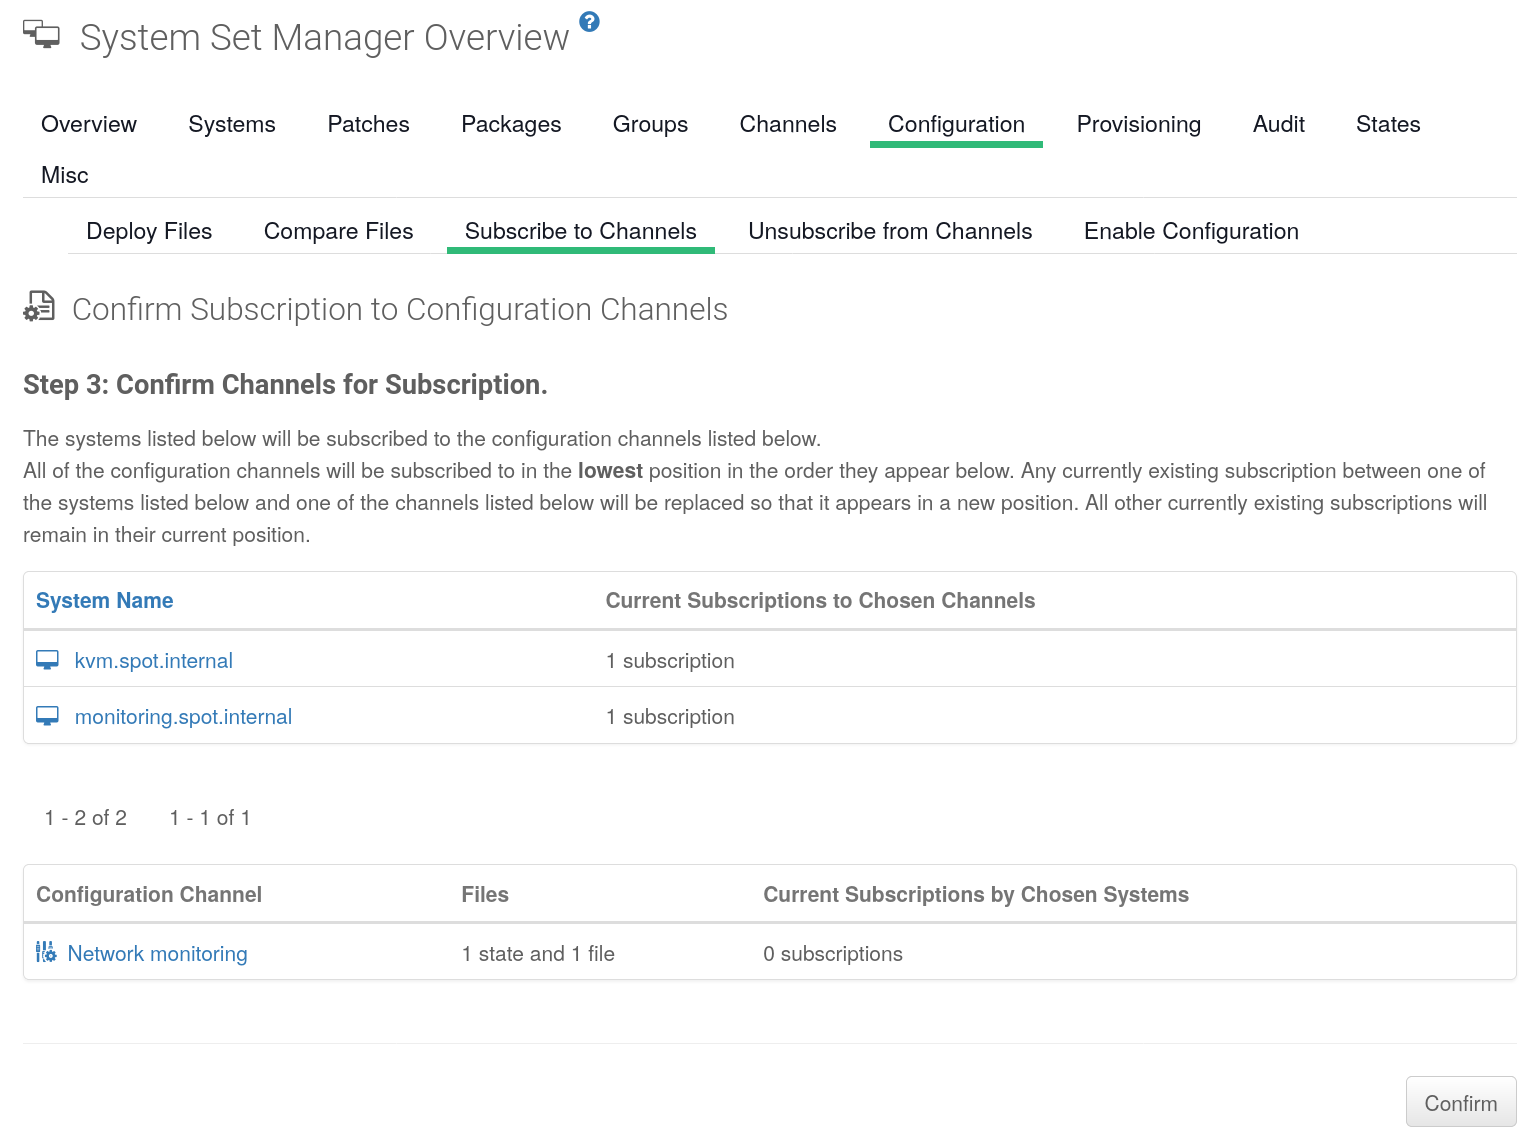
\includegraphics[width=15cm]{figures/uyuni-channelsub.png}
	\caption{Két kiszolgáló feliratkoztatása a \textit{Network monitoring} state channelre.}
	\label{fig:uyuni-channelsub}
\end{figure}

A fenti példában használt channel state fájlja \aref{lst:network-monitoring-state}.~kódrészleten látható. Ezzel néhány, a hálózati forgalom monitorozását lehetővé tevő csomagot telepítettem a feliratkozott gépekre, illetve elindítottam a kapcsolódó service-t és felülírtam az alapértelmezett konfigurációs állományt egy némileg különbözővel, ami alapértelmezetten más mértékegységeket használ a forgalom monitorozása során.

A state konfigurálásához éltem a Salt által nyújtott sablonozási lehetőséggel, mely lehetőséget biztosít például változók létrehozására, \texttt{if-else}~ágak meghatározására, és \texttt{for}~ciklus használatára is. Bár ez elsőre némi többletmunkát jelent a state létrehozása során, egy sokkal karbantarthatóbb megoldást eredményez, hiszen elegendő például a telepítendő csomagokat egy listában felsorolni, melyet bármikor bővíthetünk, és nem kell egy-egy csomópontot lemásolni újabb hibalehetőségek esetleges bevezetésével. A sablonozás további előnye, hogy futásidőben is lekérdezhetjük például egy fájl létezését, és ez alapján folytathatjuk a state végrehajtását. Ilyen megoldást szemléltet a state forráskódjának 10.~sora, melyben az elágazás megvizsgálja, hogy éppen telepítésre kerül-e a \texttt{vnstat} csomag, vagy ha nem, akkor egy létező konfigurációs állományt szeretnénk-e frissíteni. Az elágazás eredménye függvényében frissíti a fájlt, vagy változatlanul hagyja. Egy másik hatékony megoldás az úgynevezett \textit{grain}-ek használata, melyek lehetővé teszik részletes információk lekérdezését egy Salt kliensről. Ilyet használtam a forráskód 21.~sorában, ahol az~\acrshort{os}-család függvényében más-más néven tudtam elérni a vnstat háttérfolyamatát.

\lstinputlisting[caption=A Network monitoring konfigurációs csatornához tartozó Salt state.,label=lst:network-monitoring-state, numbers=left]{listings/netmonitoring-init.sls}

\section{Erőforrásigény mérése}
A fejezet elején ismertetett komoly erőforrásigény miatt kíváncsi voltam a hardver adta lehetőségek tényleges kihasználtságára. Mivel ekkor még nem állítottam be a monitoring rendszert~(ehhez előbb be kellett fejeznem az Uyuni konfigurációját), ezért egy saját Python scriptet készítettem az erőforrások állapotának figyelésére.

A mérést egy telepítőforrás-tükrözés során végeztem, hiszen ekkor volt a legnagyobb a rendszer erőforrásigénye. A jelentős mértékű hálózati adatforgalmat követően -- melyet a szoftvercsomagok letöltése idéz elő -- a rendszer hosszas adatbázis-indexelést hajt végre, mely során a processzormagok kihasználtsága közel 100\%-os. A mérési adatokból készített grafikon~\aref{fig:reposync-chart}.~ábrán látható. Jól megfigyelhető, hogy a kezdeti nagy hálózati forgalommal párhuzamosan a spacewalk kötet kihasználtsága is gyorsan nő. A letöltés befejeztével megkezdődik az adatbázis-indexelés, mely során a számítási kapacitás kihasználtságának növekedése tapasztalható, emellett pedig a várakozásoknak megfelelően az adatbázisköteten nő a foglalt terület.


\begin{figure}[ht]
	\centering
	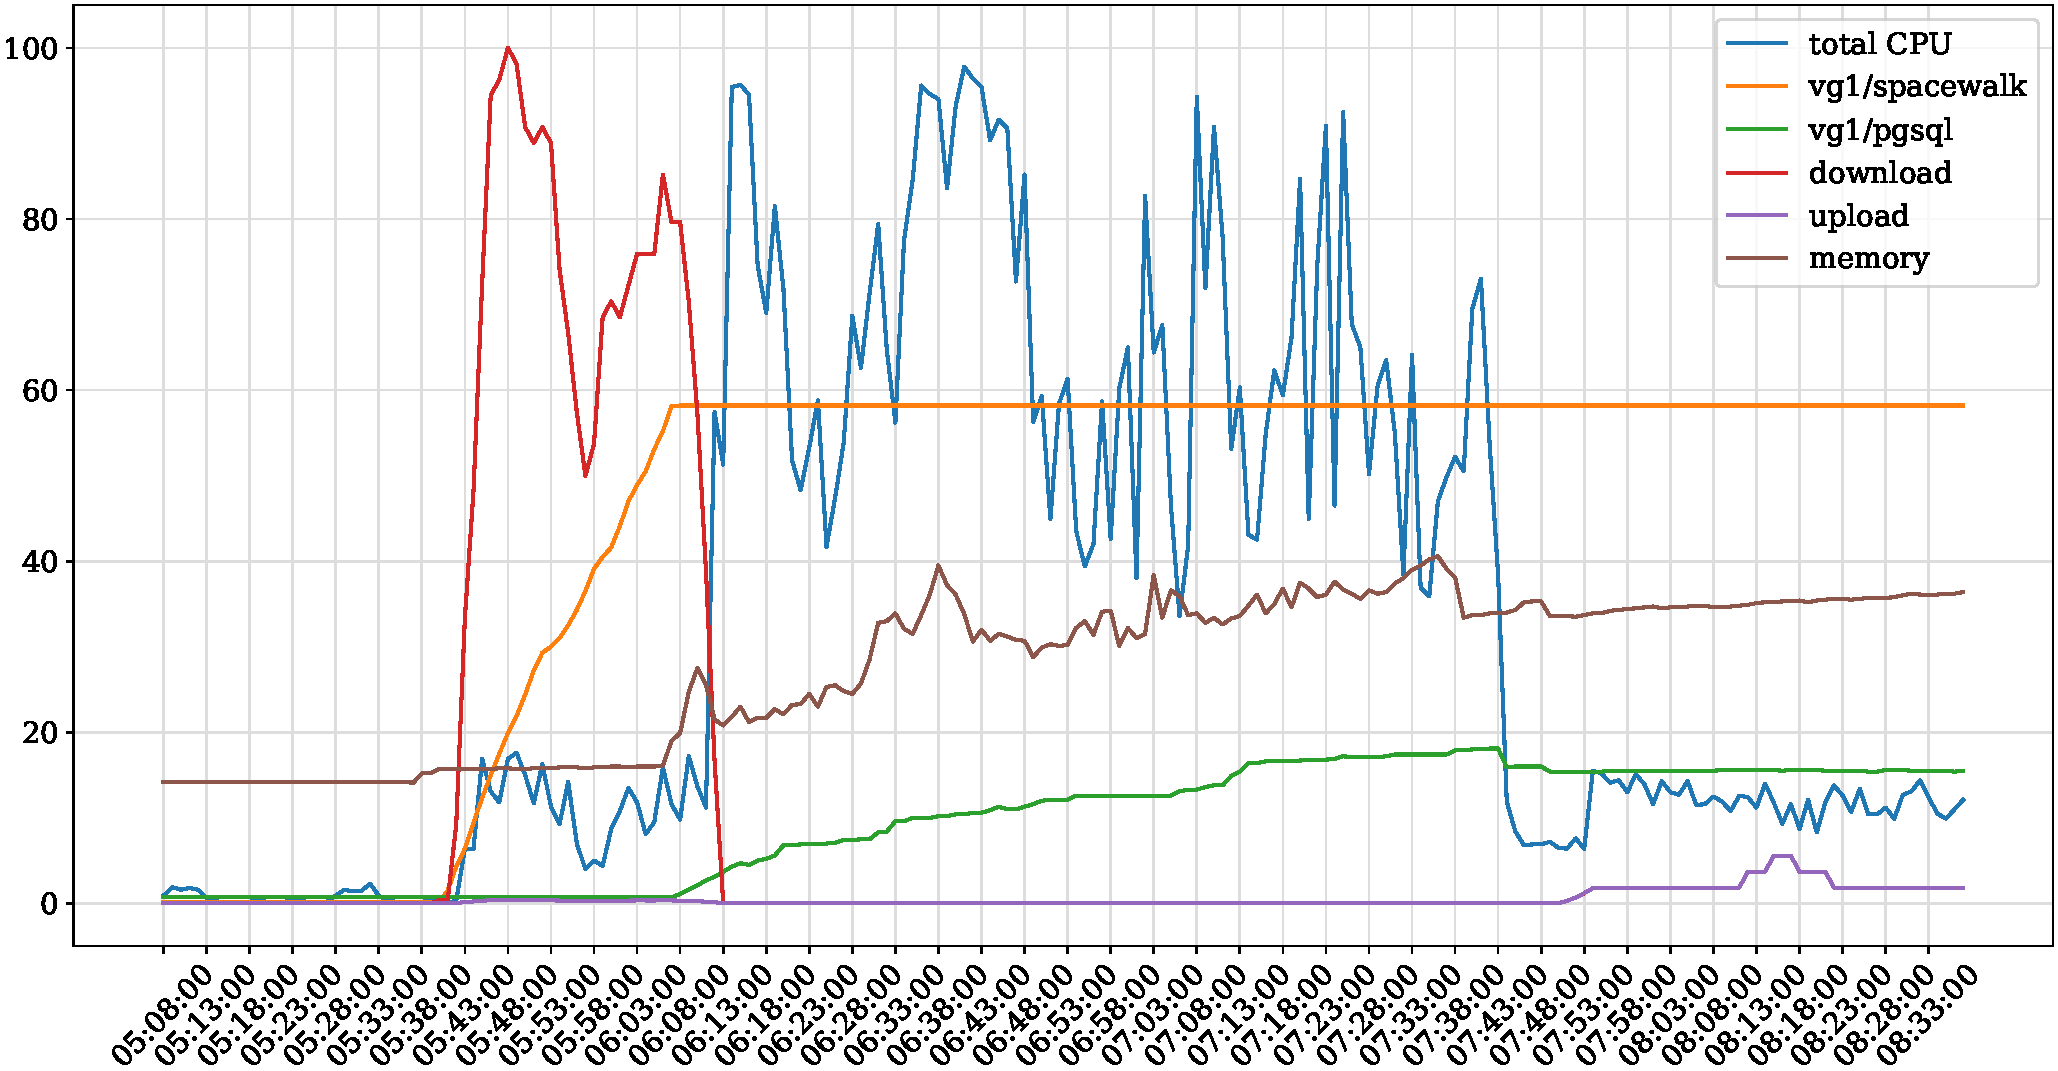
\includegraphics[width=15cm]{figures/reposync-leap-oss-grid.pdf}
	\caption{Az Uyunit futtató virtuális gép terheltsége az egyik telepítőforrás tükrözése során.}
	\label{fig:reposync-chart}
\end{figure}

Egy másik, rövidebb szinkronizálás során a virtuális gépeket futtató gazdagépen figyeltem meg a mérőszámok változását. Ennek érdekessége, hogy így lehetőségem nyílt a processzormagok hőmérsékletének nyomon követésére is. Ezáltal megfigyelhetjük a szervergép hűtésének hatékonyságát: míg a~\acrshort{cpu} kihasználtsága körülbelül 50\%-kal~nőtt, a processzor hőmérséklete csupán 8°C-kal változott, ami körülbelül 20\%-os~növekedést jelent. \Aref{fig:reposync-vhost-cputemp}.~ábráról leolvasható, hogy a processzor-hőmérséklet a~\acrshort{cpu} kihasználtságával összhangban változik, azonban érdemes megjegyezni, hogy a hőmérsékletet megjelenítéséhez egy másik skálát alkalmaztam, így a hőmérséklet-növekedés mértéke arányaiban valóban elmarad a processzorkihasználtság változásától. Az ábrán látható 60\%~körüli \acrshort{cpu}-kihasználtság egyébként közel teljes processzorkihasználtságot jelent a virtuális gépen, ugyanis ez körülbelül 14 mag teljes kihasználtságát jelenti (mivel $ 24 * 0.6  = 14,4 $), azaz a két tétlen~\acrshort{vm} mellett feltehetően az adatbázis-indexelést végző Uyunit futtató virtuális gép kihasználja a rendelkezésére álló 12~magot.

\begin{figure}[ht]
	\centering
	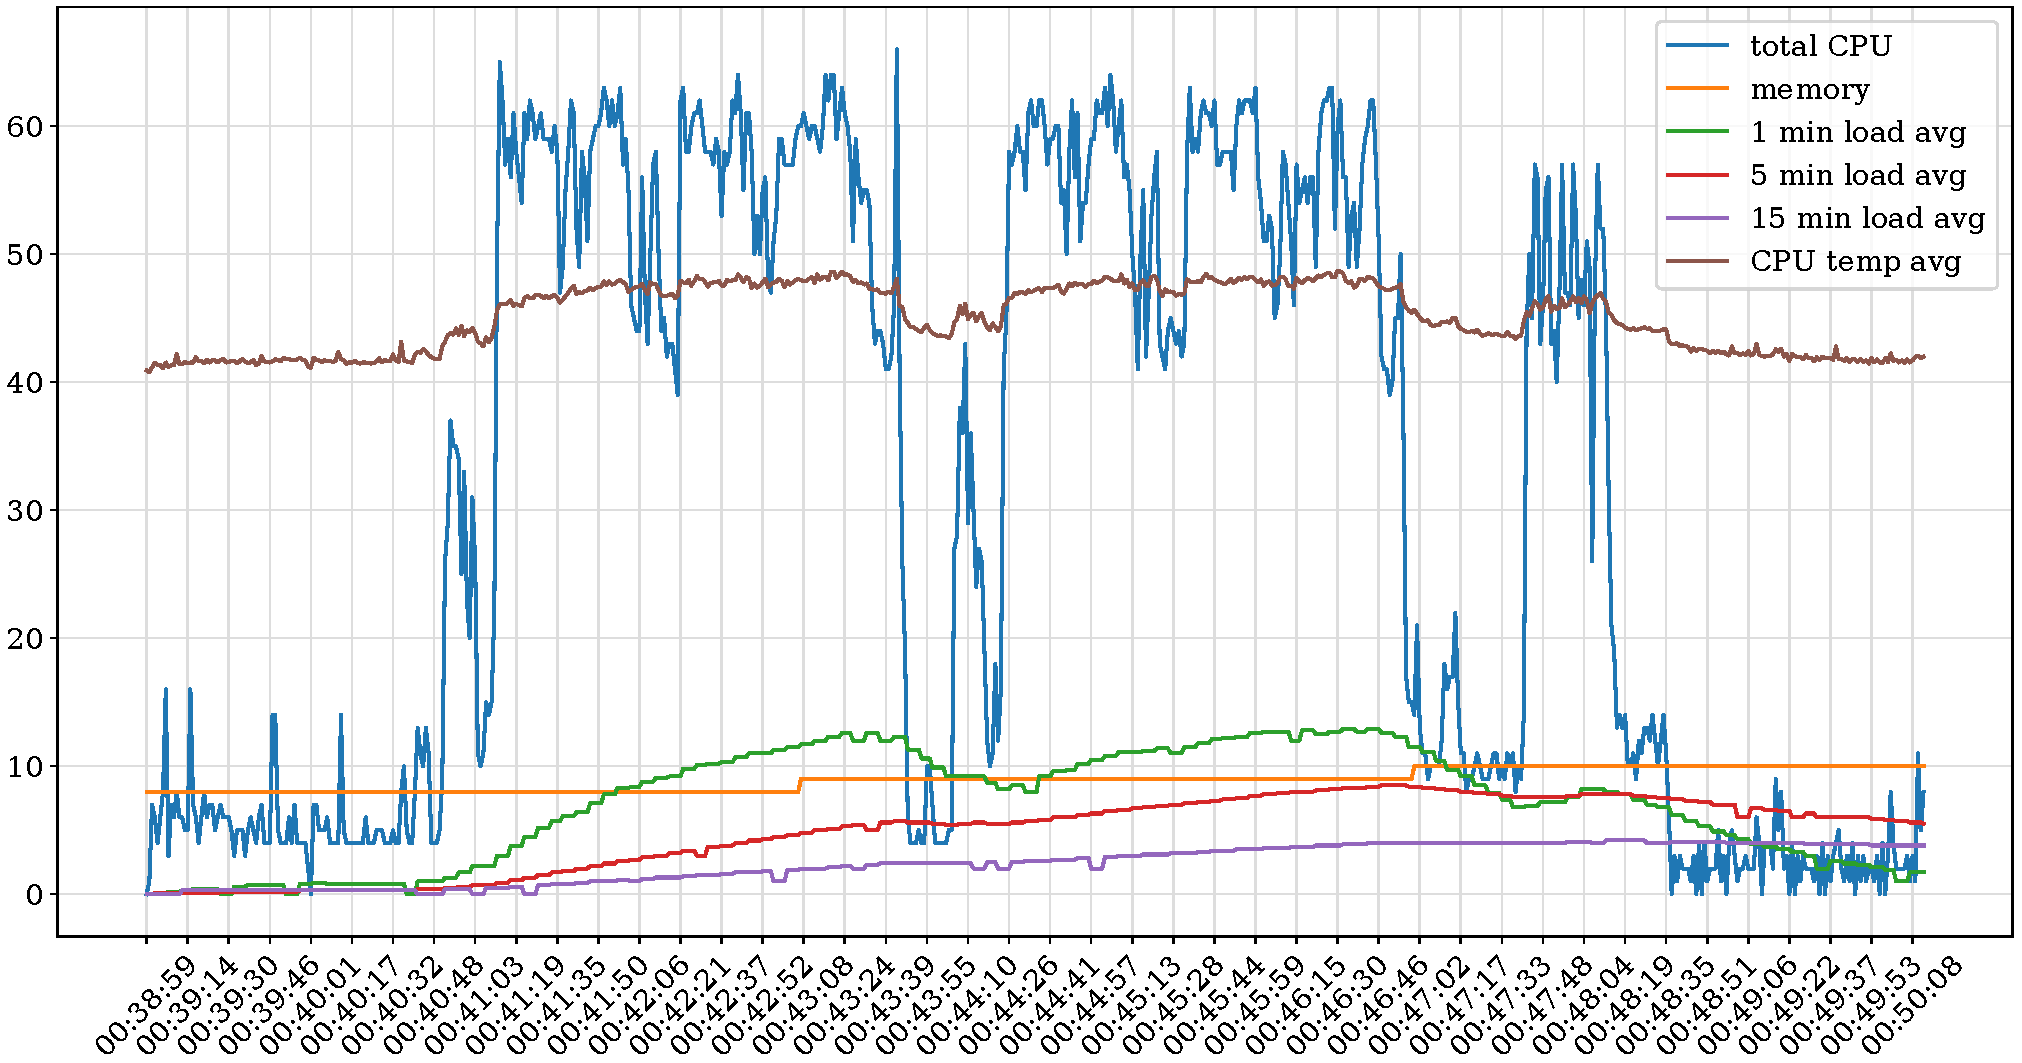
\includegraphics[width=15cm]{figures/reposync-vhost-cputemp.pdf}
	\caption{Processzormagok átlagos hőmérséklete a rendszer terheltsége mellett.}
	\label{fig:reposync-vhost-cputemp}
\end{figure}

\section{Frissítési értesítések}
Teljes körű infrastruktúramenedzsment-megoldásként az Uyuni lehetőséget biztosít a kezelt gépekre telepített csomagok állapotának folyamatos követésére: minden nap, egy előre meghatározott időpontban frissíti a telepítési források adatait, és összeveti az ezekben elérhető szoftververziókat a kezelt gépekre telepítettekével. Ennek köszönhetően a tesztkörnyezet gépeihez  frissítésekről folyamatosan értesültem e-mailben, így mindig naprakész információk álltak a rendelkezésemre a frissítéseket illetően.

Ezek közül kiemelt fontosságúak lehetnek a biztonsági frissítések, hiszen ezek között olyan sérülékenységek javításai is szerepelhetnek, mely kockázatot jelent a rendszer helyes működésére nézve. Ilyen értesítésből körülbelül két és fél hét alatt 9 érkezett, ezeken felül pedig nagyságrendileg 40~további, alacsonyabb prioritású frissítésről kaptam értesítést. Ezen felül az Uyuni felületére belépve az áttekintés oldalon és a rendszerek listájában is látható a kezelt rendszereink frissítéseinek állapota~(\ref{fig:uyuni-security-status}.~ábra).

\begin{figure}[ht]
	\centering
	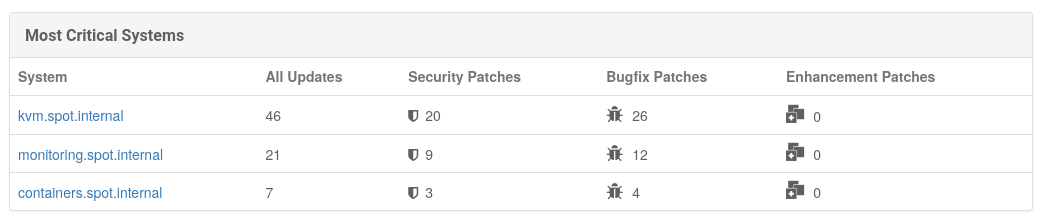
\includegraphics[width=15cm]{figures/uyuni-security-status.png}
	\caption{A kezdőlapon tájékozódhatunk a kliensek biztonsági állapotáról.}
	\label{fig:uyuni-security-status}
\end{figure}
% !TeX encoding = UTF-8
% !TeX spellcheck = hu_HU

\chapter{Monitoring}
\label{chap:monitoring}
\Aref{sect:monitoring}.~alfejezetben ismertetett előnyei miatt a tesztkörnyezetben is egy monitoring rendszer kialakítása mellett döntöttem. Választásom a Prometheus monitorozó rendszerre esett, mely a Grafana vizualizációs eszközzel társítva jó betekintést enged az üzemeltetett rendszerek állapotába. A választásomat az indokolta, hogy ez a párosítás manapság nagyon elterjedt, széles körben használt és jól kibővíthető további adatok monitorozásával, továbbá számos segédanyag áll hozzá rendelkezésre mind a hivatalos oldalon, mind pedig a közösség által karbantartott ismertetők formájában.

\section{Áttekintés}
A továbbiakban tárgyaltak könnyebb megértése végett hasznos megismerni a Prometheus és a kapcsolódó komponensek működését. A Prometheus működési elve egyszerű és hatékony: a figyelt kliensekre úgynevezett \textit{exporter}eket telepítünk, melyeket a Prometheus szerver pull modellt alkalmazva adott időközönként lekérdez. Az exporterek olyan programok, melyek alkalmasak bizonyos statisztikák (pl.~erőforráskihasználtság mértéke, adatbázis-lekérdezések gyakorisága) kiolvasására, és ezeket a monitorozott rendszer egy adott portján HTTP-protokollon keresztül közzétenni. Az exporterek önmagukban nem gyűjtenek adatokat, csak adott időközönként frissítik őket, az adatgyűjtést a Prometheus szerver végzi. Figyelt végpontokból rendszerenként több is lehet, mindegyikhez külön-külön port kapcsolódik.

A monitorozás szerves része a riasztások küldése, hiszen a monitoring rendszer folyamatos figyelése nélkül is jó, ha értesülünk a fennálló problémákról, hogy még időben be tudjunk avatkozni. A Prometheus a riasztások kezeléséhez az Alertmanager komponenst kínálja. Ezt részletesen konfigurálhatjuk az igényeinknek megfelelően, hogy milyen típusú problémáról, milyen platformon keresztül és kik kapjanak értesítést. Ez azért is kedvező, mert például egy éles környezet esetében egy alkalmazás összeomlásakor feltehetőleg másnak kell eljárnia, mint amikor hálózati fennakadást (pl.~\acrshort{dns}-probléma\footnote{A~\acrshort{dns} az emberek által könnyen megjegyezhető domain neveket fordítja le az informatikai eszközök által értelmezhető IP-címekre.}) tapasztalunk.

Az összegyűjtött adatokat a Grafana segítségével tehetjük átláthatóbbá, valamint ez teszi könnyebbé a metrikák elemzését is. Adatvizualizációra specializálódott szoftver lévén a Grafana rengeteg opcióval rendelkezik az adatok megjelenítését illetően, így a \acrshort{cpu}-adatok vonalgrafikonon való megjelenítésétől kezdve a szerverünk elérhetőségét jelző igen-nem panelt is választhatunk.
Grafanában a megjelenített adatokat -- melyekhez egy-egy panel tartozik -- úgynevezett \textit{dashboard}okba szervezhetjük. A dashboardok általában összetartozó adatokat tartalmaznak, azaz jó gyakorlat a hardveres erőforrások metrikáit külön dashboardba szervezni például a webszerverhez tartozó mérőszámoktól. % TODO: összesítés dashboard, amin a monitorozott hosztok adatai egy helyen láthatóak?
A Grafana támogatja a Prometheus saját lekérdezőnyelvével, a PromQL-lel való adatszűrést, mely lehetővé teszi a Prometheus szerverrel való egyszerű interakciót.
\Aref{fig:prometheus-architecture}.~ábra egy általános Prometheus-alapú, Grafana adatvizualizációt használó monitoring-architektúrát mutat be.

% tikz ábra beszúrása
\vspace{0.25cm}
\begin{figure}[ht]
	\centering
	\begin{tikzpicture}[node distance=5cm]
	% Define styles
	\tikzstyle{rect} = [rectangle, draw, minimum width=4.2cm, minimum height=2cm, text centered, font=\fontsize{12}{12}\selectfont]
	\tikzstyle{arrow} = [->,>=stealth]
	
	% Nodes
	\node (monitored-host) [rect, rounded corners, align=center, double copy shadow, fill=white] {Monitorozott\\szolgáltatások\\(exporterek)};
	\node (prometheus) [rect, rounded corners, below right of = monitored-host, yshift=-0.5cm] {Prometheus szerver};
	\node (alertmanager) [rect, rounded corners, above right of = prometheus, yshift=0.5cm, align=center] {Prometheus\\Alertmanager};
	\node (grafana) [rect, rounded corners, below of = prometheus, yshift=1cm] {Grafana};
	
	% Arrows
	\draw [arrow] (prometheus) to node[midway, fill=white, inner sep=2pt, align=center] {Metrikák lekérdezése\\(HTTP-kérések)} (monitored-host);
	\draw [arrow] (prometheus) to node[midway, fill=white, inner sep=2pt] {Riasztások} (alertmanager);
	\draw [arrow] (grafana) to node[midway, fill=white, inner sep=2pt] {Adatok lekérdezése} (prometheus);
\end{tikzpicture}

	\caption{A Prometheus monitoring rendszer felépítése~\cite{PrometheusIntro}.}
	\label{fig:prometheus-architecture}
\end{figure}

A Prometheus exporterek egy speciális formátumban teszik közzé az általuk kinyert adatokat. A legegyszerűbb esetben ezek szóközzel elválasztott kulcs-érték párok. Ilyen adatpárra mutat példát \aref{lst:prometheus-data-format}.~kódrészlet első~sora. A mérőszám elnevezése után kapcsos zárójelekbe szűrőket~(filter) helyezhetünk, ahogy az \aref{lst:prometheus-data-format}.~kódrészlet második~sorában is látható. Lekérdezés esetén az adatokat ugyanezzel a szintaktikával szűrhetjük.
% TODO: lekérdezésre példa

\begin{lstlisting}[caption=Prometheus exporterek által közzétett adatok.,label=lst:prometheus-data-format, numbers=left]
	node_load1 0.35
	node_hwmon_temp_celsius{chip="platform_coretemp_1",sensor="temp2"} 28
\end{lstlisting}

\section{Telepítés, konfiguráció}
\label{sect:monitoring-installation}
A környezet beüzemelését nagyban segítette, hogy a Prometheus monitoring rendszert az Uyuni külön Salt~Formulákon keresztül támogatja. Így lehetőség van az infrastruktúramenedzsment rendszerbe bevont klienseken manuális csomagtelepítés nélkül egy kezdetleges monitoring környezetet kialakítani. Ez a gyakorlatban azt jelentette, hogy az Uyuni a beállított Formulák alapján a kliensekre telepítette az alapvető rendszerinformációkat lekérdező \textit{Node exportert}, míg a monitoring szerveren egy alapbeállításokkal rendelkező Prometheus szervert és a hozzá kapcsolódó Grafana szervert telepítette.

% TODO: nagyobb betűméret a képen
\begin{figure}[ht]
	\centering
	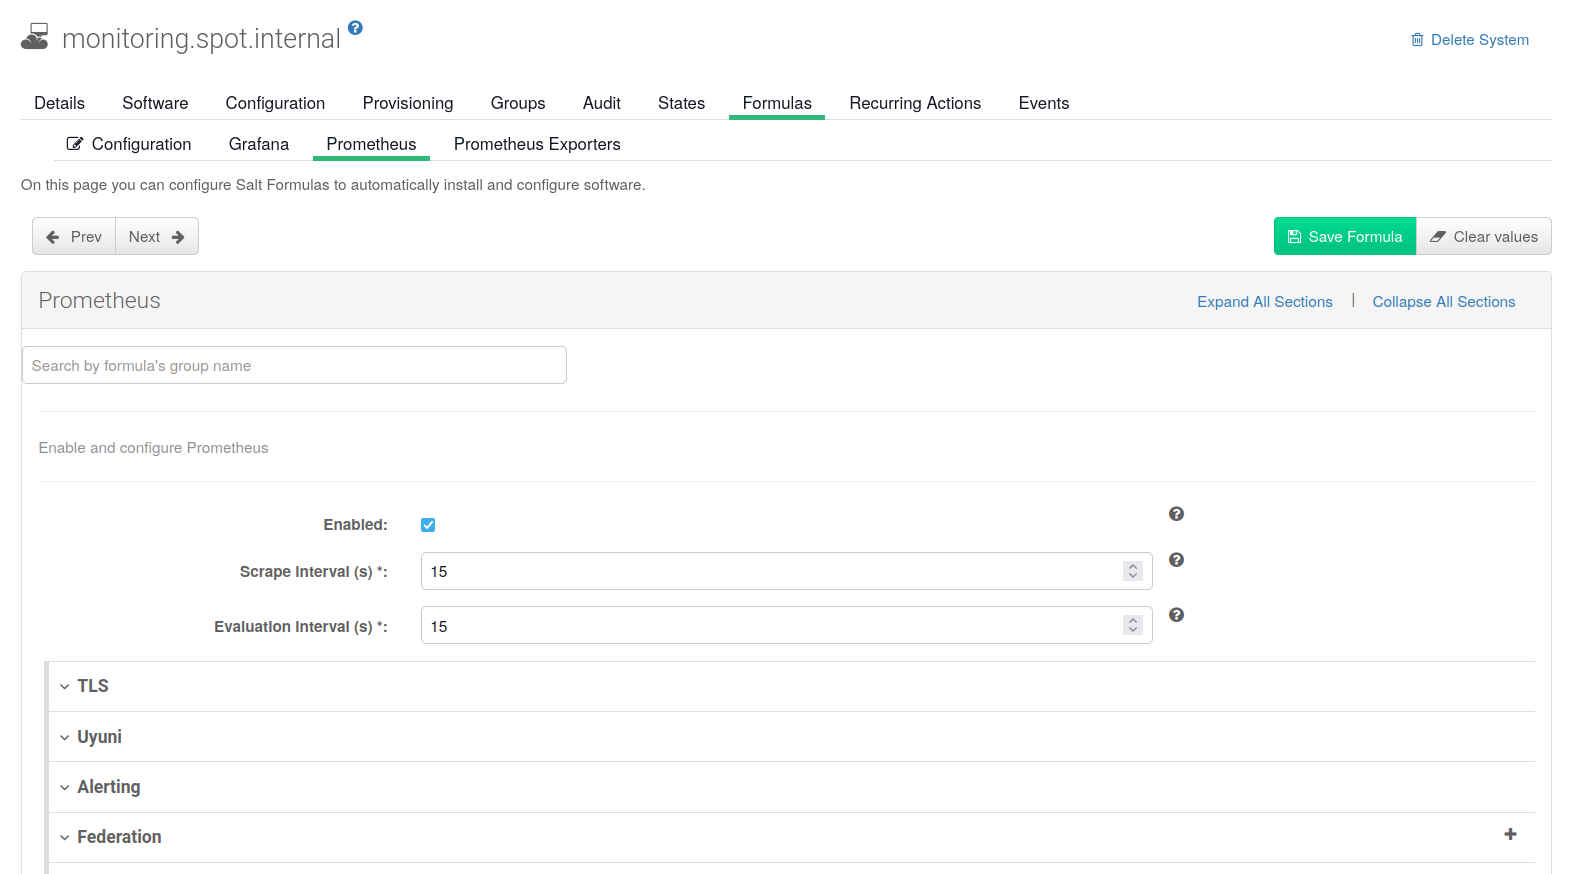
\includegraphics[width=15cm]{figures/prometheus-formula.png}
	\caption{Az Uyuni webes felületéről könnyen módosíthatjuk a Prometheus szerver alapvető beállításait.}
	\label{fig:prometheus-formula}
\end{figure}

\subsection{Konténerhoszt monitorozása}
A monitoring rendszer kialakítása során nehézséget jelentett, hogy openSUSE Leap Micro-ra nem volt hivatalosan elérhető a felügyelt gépekről hardver- és kernelstatisztikákat szolgáltató Node exporter szoftvercsomag formájában. Emiatt eleinte a konténerhoszt monitorozására nem volt lehetőségem. A megoldást az jelentette, hogy az exportert egy konténerben telepítettem a virtuális gépre. Mivel a konténer azonban a gazdagéptől elkülönülten fut, ezért módosítani kellett a konténer futtatásához használt parancsot. A \texttt{--path.rootfs=/host} kapcsoló beállításával az exporter már a konténerből is képes volt elérni a gazdagép metrikáit, így ezt a hosztot sikerült bevonni a monitoring rendszerbe.

\subsection{Tűzfal beállítása}
Az operációs rendszerek telepítése során a tűzfal engedélyezését választottam. Ez azt jelentette, hogy szinte minden port zárva volt a külvilág felé, így a Prometheus szerver sem tudta elérni az exporterek által szolgáltatott adatokat.

Ahhoz, hogy a monitoring rendszer az elvárt módon működjön, szükséges volt a tűzfalszabályok módosítása. A telepített rendszereken a \texttt{firewalld} az alapértelmezett tűzfal, melynek a beállításait a \texttt{firewall-cmd} segédprogram segítségével tudtam módosítani~(\ref{lst:firewalld-add-port}.~kódrészlet első~sora). A kódrészlet harmadik sorában a szükséges portok kinyitását követő állapot látható az Uyunit futtató szerver esetében, a monitoring rendszerben használt exportereket, rövid leírásukat és a kapcsolódó portszámokat \aref{tab:monitoring-exporters}.~táblázat tartalmazza. A monitoring szerverhez tartozó Salt~Formula alkalmazásával automatikusan telepítésre kerülnek a Tomcat és Taskomatic exporterek. Ezek az Uyuni alapjait adó webes keretrendszerről és a használt feladatütemezőről biztosítanak statisztikákat.

\vspace{2mm}
\begin{lstlisting}[caption=Tűzfalszabályok módosítása.,label=lst:firewalld-add-port, numbers=left,escapechar=?]
	?\underline{uyuni:$\sim$ \#}? firewall-cmd --permanent --add-port=9117/tcp
	?\underline{uyuni:$\sim$ \#}? firewall-cmd --list-ports
	5556/tcp 5557/tcp 9100/tcp 9117/tcp 9187/tcp 9800/tcp
\end{lstlisting}

\begin{table}[h]
	\setlength{\tabcolsep}{5pt}
	\renewcommand{\arraystretch}{1.3}
	\centering
	\begin{tabular}{||l l m{7.6cm}||}
		\hline
		Portszám & Exporter & Leírás \\
		\hline\hline
		5556 & Tomcat JMX exporter & Az Uyuni működéséhez szükséges Tomcat alkalmazás Java-processzéről jelenít meg adatokat (pl.~szálak, memóriahasználat). \\
		\hline
		5557 & Taskomatic JMX exporter & Az Uyuni által használt Tascomatic alkalmazás Java-processzéről jelenít meg adatokat (pl.~szálak, memóriahasználat). \\
		\hline
		9090 & Prometheus exporter & A Prometheus állapotáról tesz közzé adatokat (pl.~hibás lekérések száma, lekérések mérete).  \\
		\hline
		9100 & Node exporter & Linux hosztokról publikál számos hardver- és kernelmetrikát (pl.~erőforráshasználat, kontextusváltások). \\
		\hline
		9117 & Apache exporter & Az Apache webszerverről ad meg mérőszámokat (pl.~egyes HTTP-státuszkódokhoz tartozó lekérdezések száma, \acrshort{cpu}-idő).  \\
		\hline
		9187 & PostgreSQL exporter & Az Uyuni által használt PostgreSQL adatbázismotorról oszt meg adatokat (pl.~zárak száma, rekordlekérdezési és frissítési ráta).  \\
		\hline
		9800 & Taskomatic exporter & Az Uyuni által használt Taskomatic feladatütemező metrikáit jeleníti meg (pl.~elvégzett feladatok száma, aktuális szálak száma).  \\
		\hline
	\end{tabular}
	\caption{A monitoring rendszerben használt Prometheus exporterek a hozzájuk tartozó portszámokkal.}
	\label{tab:monitoring-exporters}
\end{table}

% tikz ábra beszúrása
\begin{figure}[ht]
	\centering
	\begin{tikzpicture}[node distance=4.3cm]
	\tikzstyle{rect} = [rectangle, draw, minimum width=3.8cm, minimum height=1.8cm, text centered, font=\fontsize{12}{12}\selectfont]
	\tikzstyle{arrow} = [->,>=stealth]
	
	\node (kvm) [rect, rounded corners] {KVM-hoszt};
	\node (containers) [rect, rounded corners, right of = kvm] {Konténerhoszt};
	\node (uyuni) [rect, rounded corners, right of = containers] {Uyuni szerver};
	\node (monitoring) [rect, below of = containers, yshift=-0.5cm] {Monitoring szerver};
	
	\draw [arrow] (monitoring) to node[above left, near end, xshift=-10, yshift=-4, align=left] {9100} (kvm);
	\draw [arrow] (monitoring) to node[near end, right] {9100} (containers);
	\draw [arrow] (monitoring) to node[near end, right, align=left, xshift=18, yshift=-8] {5556, 5557\\9100, 9117\\9187.9800} (uyuni);
	\draw [arrow, loop, bend left] (monitoring.north east) to[out=150, in=60, looseness=8, align=left, xshift=3] node[right] {9090\\9100} (monitoring.east);
\end{tikzpicture}

	\caption{A monitoring rendszerbe bevont gépek a rajtuk futó exporterek által használt portokkal.}
	\label{fig:monitoring-setup}
\end{figure}

\section{Riasztások beállítása}
A Prometheus-alapú monitoring rendszer egyik legfontosabb komponense az Alertmanager, hiszen ennek segítségével a gyűjtött adatok folyamatos szemmel tartása nélkül is értesülhetünk a rendszerünket érintő lényeges eseményekről.
\Aref{fig:prometheus-architecture}.~ábrán látható, hogy az Alertmanager egy különálló modul a monitoring-infrastruktúrában. Ez a modularitás a gyakorlatban is megjelenik: az Alertmanager a Prometheustól elkülönülten, a~\texttt{golang-github-prometheus-alertmanager} csomaggal telepíthető, a telepítést követően pedig egy külön konfigurációs fájl és systemd unit fájl tartozik hozzá, azaz a Prometheus adatgyűjtő részétől elkülönülten kezelhető.

A tesztkörnyezetben az Alertmanager konfigurációját Salt state-tel végeztem. Ehhez létrehoztam egy új konfigurációs csatornát (configuration channel, \ref{fig:alertmanager-state}.~ábra), mely tartalmazta az Alertmanager konfigurációs állományát, valamint az ennek érvényre jutását biztosító state fájlt.

A riasztáskezelő alrendszer beállításának célja az volt, hogy egy monitorozott szolgáltatás elérhetetlenné válása esetén az azt figyelő rendszer küldjön értesítést e-mailben a hibáról. Ennek megvalósításához \aref{lst:alertmanager-yml-short}.~kódrészleten látható beállításokat használtam. Itt megfigyelhető a lokális \acrshort{smtp}-szerver megadása, és az értesítések küldéséhez használt e-mail cím beállítása.
Az 5.~sorban kezdődő \texttt{route} beállítás adja meg, hogy a specifikusabb szűrőkre nem illeszkedő riasztásokkal hogy járjunk el. Ebben az esetben ezeket csoportosítjuk a riasztás típusa és az azt küldő hoszt alapján. A \texttt{receivers} címkén belül adhatjuk meg, hogy a riasztásokat milyen végpontokra küldje a rendszer. A konfigurációs fájlban szereplő beállítások egy egyszerű e-mailt küldenek a megadott címre. Mivel a titkosítás használata a lokális gépen futó levelezőszerver esetében nem indokolt, és konfigurációja összetett, ezért a 13.~sorban látható \texttt{require\_tls} opcióval ezt kikapcsoltam. Fontos azonban, hogy ezt csak helyi mail szerver esetén tehetjük meg, amennyiben egy központi levelezőszervert használunk, akkor a program nem is engedi a titkosítás kikapcsolását~\cite{PrometheusAlertmanagerConfig}.
A 14.~sorban látható \texttt{send\_resolved} opciót igazra állítva a szolgáltatások helyreállásáról is kapunk értesítést. % TODO: példa riasztás email?

A teljes, kommentekkel ellátott konfigurációs fájl elérhető a \textbf{Függelék}ben. % TODO: függelékbe

% TODO: kép nagyítása
\begin{figure}[ht]
	\centering
	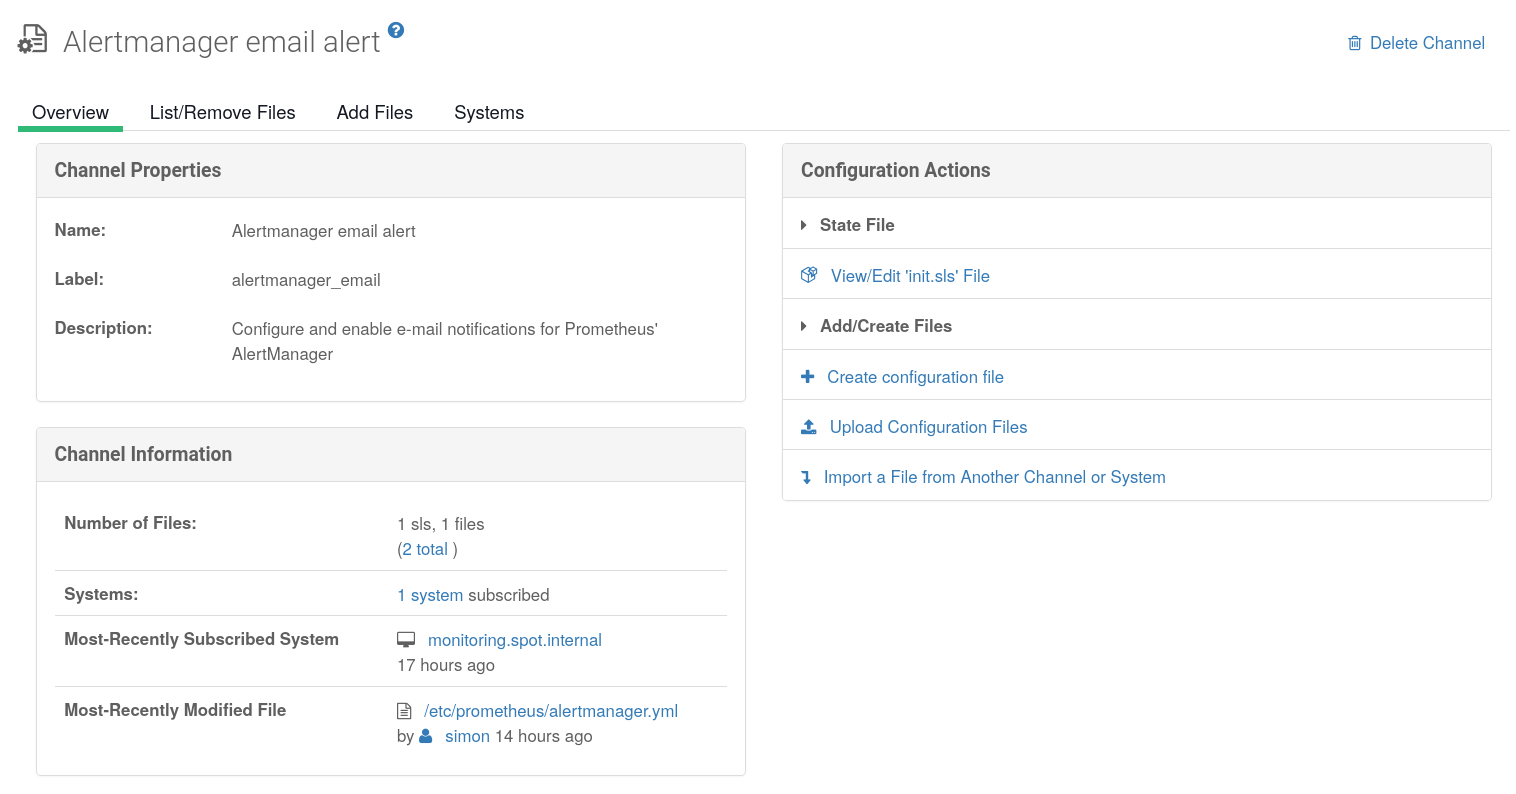
\includegraphics[width=15cm]{figures/alertmanager-state.png}
	\caption{A monitoring értesítések kezeléséhez használt Salt state.}
	\label{fig:alertmanager-state}
\end{figure}

% TODO: oldaltörés javítása?
% TODO: a teljes kódrészlet legyen a függelékben
% https://tex.stackexchange.com/a/224743
\lstinputlisting[caption=Az e-mail-értesítések küldéséhez használt konfigurációs fájl részlete.,label=lst:alertmanager-yml-short, numbers=left]{listings/alertmanager.yml.short}

A fent ismertetett konfigurációs fájlt \aref{lst:alertmanager-state}.~kódrészleten szereplő Salt state-tel telepítettem a monitoring szerverre. Ehhez a Salt által fájlok kezelésére nyújtott \texttt{file.managed} state opciót használtam, majd a kódrészlet 4.~sorában szereplő \texttt{source} címkével megadtam az Uyuni által kezelt leírófájlt, valamint beállítottam a telepítendő fájl elérési útját és a kapcsolódó jogosultságokat (\ref{lst:alertmanager-state}.~kódrészlet 5-7.~sora). 
A Salt-tal való konfiguráció-menedzsment a \texttt{service.running} state opcióval lehetőséget kínál a kapcsolódó service újratöltésére, amit a \texttt{watch} opció beállításával automatikusan is megtehetünk. Így tehát a kódrészlet 16.~sorában megadott fájl módosulása esetén az alertmanager-t futtató systemd service automatikusan újraindításra kerül a módosítások érvényre juttatásával, ezzel is csökkentve a manuális beavatkozás szükségességét.

\lstinputlisting[caption=Az e-mail-értesítések beállítását végző konfigurációs állomány telepítéséhez használt Salt state.,label=lst:alertmanager-state, numbers=left]{listings/alertmanager-init.sls}


\section{Adatvizualizáció}
A gyűjtött adatok áttekintése, elemzése segítségünkre lehet további rendszerek telepítése során például szükséges erőforrások mennyiségének becsléséhez, illetve szolgáltatáskiesést követően segíthet a probléma meghatározásában.

\Aref{sect:monitoring-installation}.~alfejezetben ismertetettek alapján a tesztkörnyezetben a Grafana adatvizualizációs eszközt használtam. Ez jó integrációt biztosít a Prometheushoz, könnyen lekérdezhetőek a különböző metrikák. A telepítéshez használt Salt~Formula pedig még egyszerűbbé tette a Grafana használatát: az alapértelmezett konfigurációs fájl számos előre definiált, a rendszerek állapotát jól összefoglaló dashboardot tartalmaz, így a tűzfalbeállításon és néhány panel webes felületen történő személyre szabásán túl nem volt szükséges részletesebben konfigurálni.

\Aref{fig:grafana-uyuni-server}.~ábrán látható dashboard az Uyuni szerver állapotát ismerteti. Ez a dashboard is a Grafana Salt Formula része, néhány panel mértékegységének pontosításán és skálázásán kívül nem volt szükség a beállítások módosítására. Az ilyen nézetek előnye, hogy segítségükkel nagyon hamar megállapíthatjuk a rendszereink állapotát, hiszen minden lényeges mérőszámot tartalmaznak: segítségével figyelemmel követhetjük például a rendszer terheltségét, a processzor és a memória kihasználtságát, a hálózat- és háttértárhasználat rátáját, az adatbázis-műveletek állapotát és a háttértárak kihasználtságát.

\begin{figure}[ht]
	\centering
	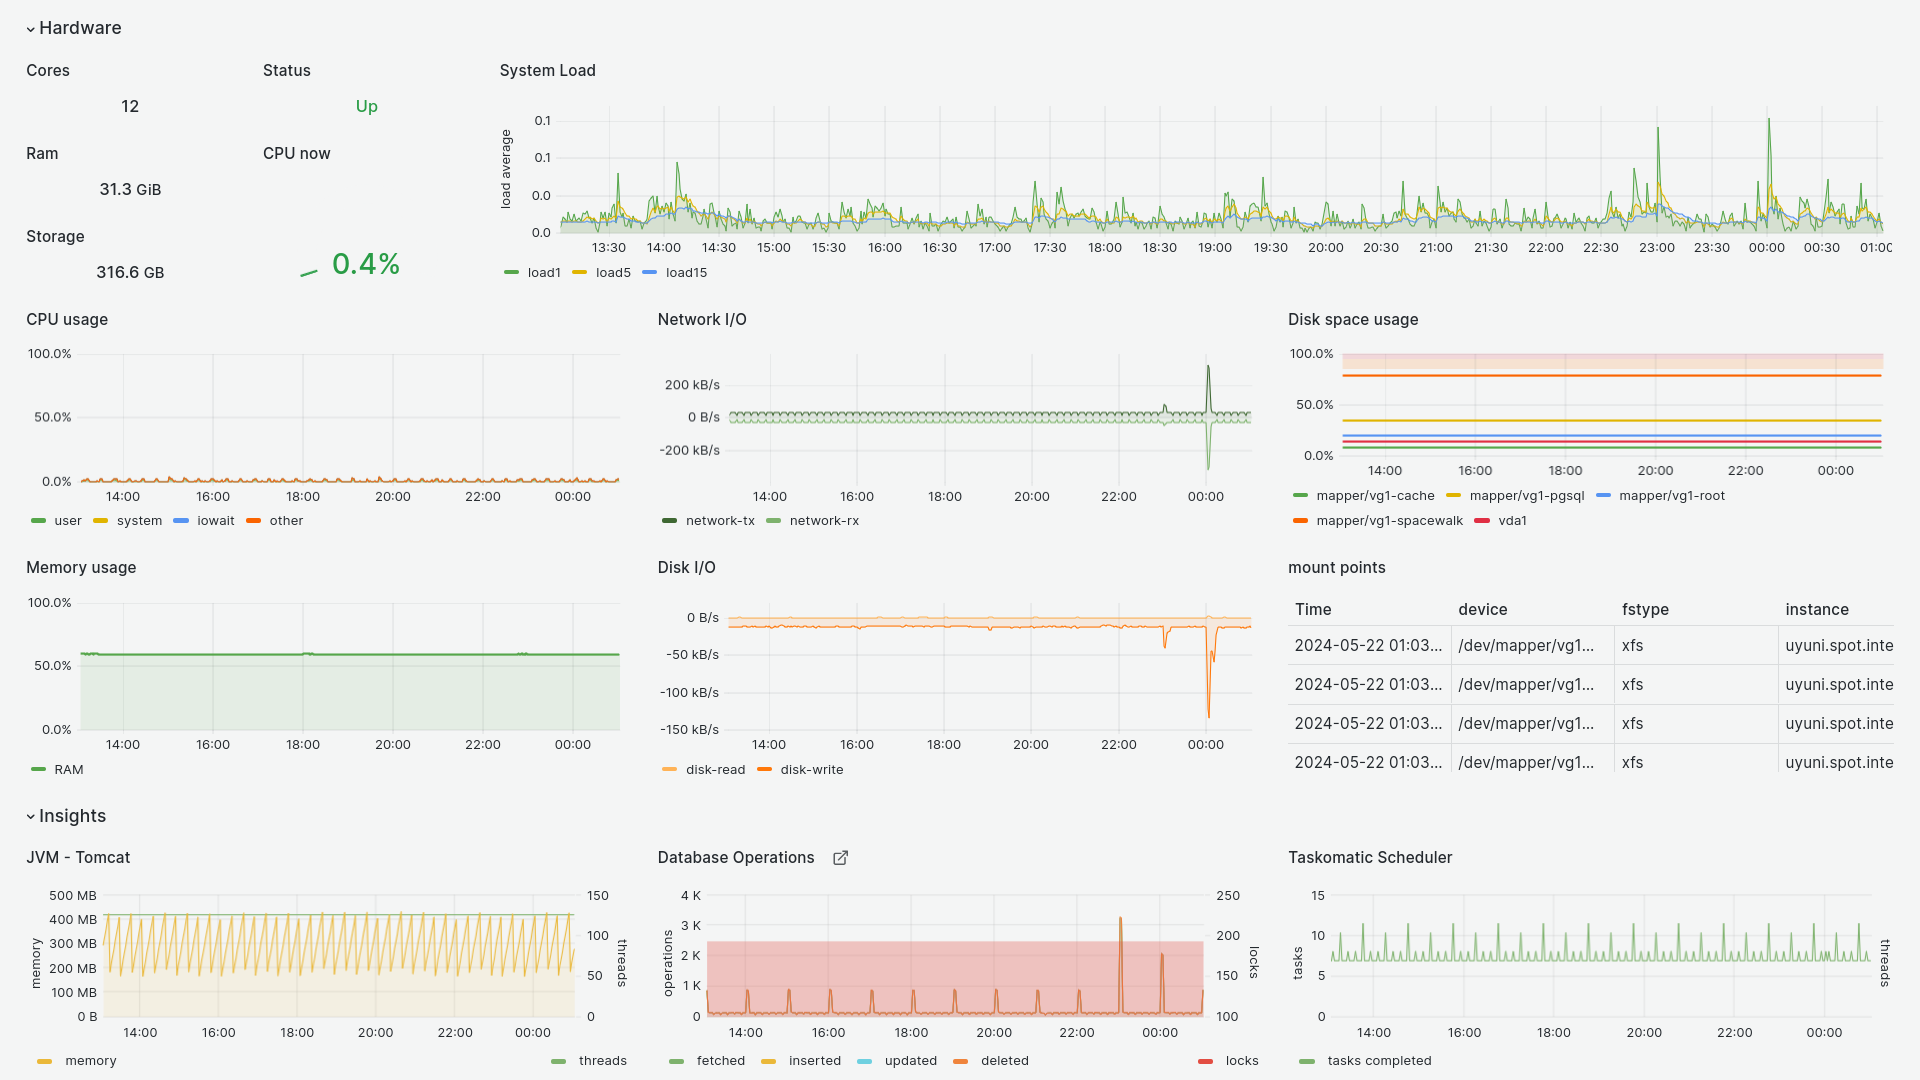
\includegraphics[width=15cm]{figures/grafana-uyuni-server.png}
	\caption{A tesztkörnyezetben használt Grafana egyik dashboardja az Uyuni szerver fontosabb mérőszámait mutatja be.}
	\label{fig:grafana-uyuni-server}
\end{figure}

% TODO: két-két és fél számmal?
Bár a tesztkörnyezet körülbelül két-két és fél hónapos folyamatos üzemeltetése során nem voltak jelentős kimaradások, az Uyuni kezdetleges konfigurációja során az egyik telepítőforrás tükrözése során többször is leállt az azt futtató gép, így valós helyzetben nyílt alkalmam a metrikák visszanézésére, és a hiba okának felkutatására. Az incidens során megjelenő grafikont \aref{fig:reboot-grafana}.~ábra mutatja be. A grafikon jobb oldalán látható a négy leállás, a bal szélén pedig láthatjuk, hogy néhány órával korábban hasonlóan magas terhelés mellett nem lépett fel a hiba. A grafikon $ y $ tengelyén láthatjuk, hogy az nem 100\%-ig, hanem sokkal tovább fut. Ennek oka, hogy a rendszerterhelés számítása során az egy processzormagra eső maximális terhelést tekintjük a 100\%-nak, így egy 24~\acrshort{cpu}-val rendelkező gép esetén a maximális érték 2400\% lenne. A grafikonon 1600\%~körülre esik a legnagyobb terhelés, ami összhangban van az Uyunit futtató virtuális gép által maximálisan használható 16~processzormaggal. Mint később kiderült, a hibát hardveres hiba okozta, a virtuális gép által használható processzormagok csökkentésével a probléma nem jelentkezett többé.

\begin{figure}[ht]
	\centering
	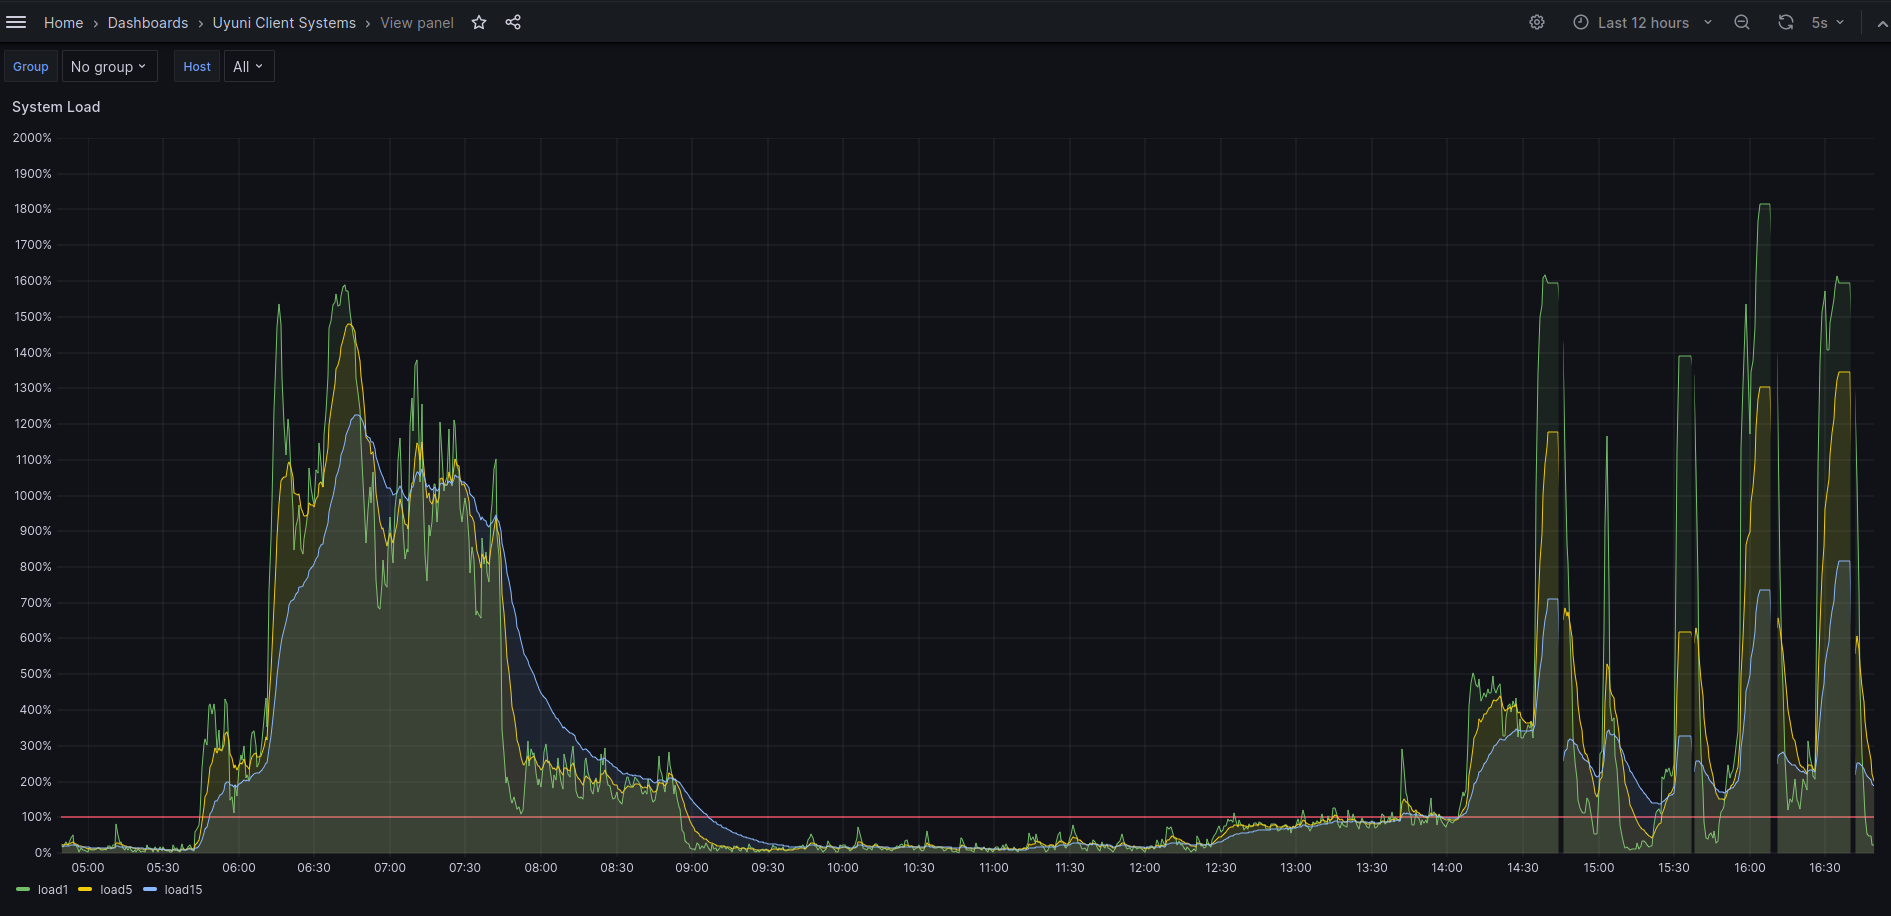
\includegraphics[width=15cm]{figures/reboot-grafana.png}
	\caption{A telepítőforrás-tükrözés során tapasztalt szolgáltatáskiesések a Grafanaban megjelenő grafikonon.}
	\label{fig:reboot-grafana}
\end{figure}

% !TeX encoding = UTF-8
% !TeX spellcheck = hu_HU

\chapter{Összefoglalás}

\section{Elért eredmények}
Dolgozatomban egy átfogó képet adtam a nagyvállalati rendszerek üzemeltetése során felmerülő kihívásokról, ezek lehetséges hatékony megoldásairól. Részletesen kitértem a kötetkezelés, az infrastruktúra-menedzsment és a monitoring témakörökre, melyek egy nagy méretű infrastruktúra üzemeltetésének elengedhetetlen kellékei. Ismertettem néhány konkrét megoldást, egy kis méretű tesztkörnyezetben bemutattam ezek alkalmazási lehetőségeit, a~tesztrendszer komponenseihez kapcsolódóan méréseket végeztem.

Munkám során megismerkedtem számos elterjedt technológiával, és mélyrehatóan tanulmányoztam ezeket. A téma jó dokumentáltsága lehetőséget nyújtott arra, hogy több különböző forrásból szerezzek információkat a megoldásokat illetően, és részletesen megismerkedjek egy-egy technológiával. Az ismeretek elsajátításához nagyban hozzájárultak a szoftvergyártók és a termékek hivatalos írásai, melyek magas minőségű tananyagoknak bizonyultak. A megismert lehetőségek megértésében nagy szerepet játszott a tesztkörnyezet, melyben alkalmam nyílt a megoldások kipróbálására, és szabadon kísérletezhettem a~különböző eszközökkel.

\section{Továbbfejlesztési lehetőségek}
Az értekezésem során részletesen tárgyaltam a kötetkezelés és az adattárolás témakörét, de~a~tesztkörnyezetben nem volt lehetőségem sem RAID-megoldás alkalmazására, sem pedig valamilyen biztonságimentés-szolgáltatás telepítésére vagy igénybe vételére. Úgy gondolom, hogy ezek egy valós környezetben elengedhetetlenek, hiszen egy adatvesztés további súlyos problémákat okozhat, ezért fontos, hogy egy szervezet mindig fel legyen készülve az adatok visszaállítására, akár hardveres meghibásodás, akár rosszindulatú támadás okozta azt. Emiatt fontosnak tartom egy backup-keretrendszer megismerését, egy mentési stratégia kialakítását.

Ahogy már többször említettem a dolgozatom során, egy nagyvállalati környezetben nem ritka, hogy több száz vagy akár több ezer gépet kell kezelnünk. A tesztkörnyezetben ehhez képest mindössze három virtuális gépet és egy fizikai gépet üzemeltettem. Értelemszerűen nem reális, hogy egy ilyen jellegű környezetbe több száz gépet telepítsünk, de~úgy~gondolom, hogy például az infrastruktúra-menedzsment eszközök képességei jobban bemutathatóak lettek volna, ha néhány géppel többet tudok kezelni (pl.~egy külön webszervert, egy adatbázisszervert és egy levelezőkiszolgálót). Mindemellett ezen rendszerek konfigurálása és összehangolása jelentős többletmunkával járt volna, helyes beállításuk (ide~értve például a megfelelő titkosítási eljárások alkalmazását) körülbelül az eddig létrehozott környezettel azonos időt igényelt volna.

A lehetőségek tanulmányozása során nagyon tetszett Salt state-ek sokszínűsége, hogy egy pár soros leírófájllal mennyi mindent meg lehet oldani, viszonylag komplex dolgokat is. Biztos vagyok benne, hogy az itt érintettnél sokkal nagyobb mélységekbe lehet bocsátkozni a technológiát illetően, így a Salt-leírók továbbfejlesztése, szélesebb körű használata is jó kihívásnak ígérkezik.

A monitoring rendszer rendkívül sok irányban továbbfejleszthető, például Grafanaban számtalan lehetőség áll rendelkezésünkre további adatok megjelenítésére, a Prometheusba bevonhatunk újabb exportereket, és az Alertmanager segítségével finomíthatjuk a riasztások kezelését (pl.~más platformokon is jelezzen, vagy beállíthatunk részletesebb szűrést).

Láthatjuk, hogy a technológia fejlődésével és a trendek folyamatos változásával --~például a manapság egyre népszerűbb konténerizációs megoldások népszerűségének növekedésével~-- a lehetőségek határtalanok, az eddigi munkám számos módon kiegészíthető.


% Acknowledgements
%~~~~~~~~~~~~~~~~~~~~~~~~~~~~~~~~~~~~~~~~~~~~~~~~~~~~~~~~~~~~~~~~~~~~~~~~~~~~~~~~~~~~~~
%----------------------------------------------------------------------------
\chapter*{\koszonetnyilvanitas}\addcontentsline{toc}{chapter}{\koszonetnyilvanitas}
%----------------------------------------------------------------------------

Ez nem kötelező, akár törölhető is. Ha a szerző szükségét érzi, itt lehet köszönetet nyilvánítani azoknak, akik hozzájárultak munkájukkal ahhoz, hogy a hallgató a szakdolgozatban vagy diplomamunkában leírt feladatokat sikeresen elvégezze. A konzulensnek való köszönetnyilvánítás sem kötelező, a konzulensnek hivatalosan is dolga, hogy a hallgatót konzultálja.


% List of Figures, Tables
%~~~~~~~~~~~~~~~~~~~~~~~~~~~~~~~~~~~~~~~~~~~~~~~~~~~~~~~~~~~~~~~~~~~~~~~~~~~~~~~~~~~~~~
%\listoffigures\addcontentsline{toc}{chapter}{\listfigurename}
%\listoftables\addcontentsline{toc}{chapter}{\listtablename}

\printindex
\printglossaries


% Bibliography
%~~~~~~~~~~~~~~~~~~~~~~~~~~~~~~~~~~~~~~~~~~~~~~~~~~~~~~~~~~~~~~~~~~~~~~~~~~~~~~~~~~~~~~
%\addcontentsline{toc}{chapter}{\bibname}
\addcontentsline{}{chapter}{\bibname}
\bibliography{bib/mybib}


% Appendix
%~~~~~~~~~~~~~~~~~~~~~~~~~~~~~~~~~~~~~~~~~~~~~~~~~~~~~~~~~~~~~~~~~~~~~~~~~~~~~~~~~~~~~~
% % !TeX encoding = UTF-8
% !TeX spellcheck = hu_HU
%----------------------------------------------------------------------------
\appendix
%----------------------------------------------------------------------------
\chapter*{\fuggelek}\addcontentsline{toc}{chapter}{\fuggelek}
\setcounter{chapter}{\appendixnumber}
\label{cha:appendix}
%\setcounter{equation}{0} % a fofejezet-szamlalo az angol ABC 6. betuje (F) lesz
\numberwithin{equation}{section}
\numberwithin{figure}{section}
\numberwithin{lstlisting}{section}
%\numberwithin{tabular}{section}
\linespread{1}

%----------------------------------------------------------------------------
\section{A monitoring beállítása előtti adatgyűjtéshez használt program}
%----------------------------------------------------------------------------
\lstinputlisting[caption={A monitorozáshoz készített, psutil csomagot használó Python-script, mely csv formátumban menti el a metrikákat.},label=lst:python-sysstats,language=Python, numbers=left]{listings/sysstats.py}


%----------------------------------------------------------------------------
\clearpage\section{E-mail-értesítések beállítását tartalmazó konfigurációs állomány}
%----------------------------------------------------------------------------
\lstinputlisting[caption={A monitoring rendszerben e-mail-értesítések küldésére használt konfigurációs fájl.},label=lst:alertmanager-config-full,numbers=left]{listings/alertmanager.yml}


%\label{page:last}
\end{document}
